\documentclass[10pt,twocolumn,letterpaper]{article}

% --- Page Geometry & Conference Margins ---
\usepackage[top=0.75in,bottom=0.85in,left=0.75in,right=0.75in]{geometry}
\setlength{\columnsep}{0.25in}

\usepackage{mathptmx}
\usepackage{microtype}
\usepackage{graphicx}
\usepackage[export]{adjustbox}
\usepackage{amsmath}
\usepackage{amssymb}
\usepackage{booktabs}
\usepackage{url}
\usepackage{cite}
\usepackage{xcolor}
\usepackage{placeins}
\usepackage{caption}
\usepackage{enumitem}
\usepackage{titlesec}
\usepackage{tabularx}
\usepackage{multirow}
\usepackage{hyperref}

% --- Ragged bottom and paragraph tolerance for 2-column formatting ---
\raggedbottom
\emergencystretch=2em
\hbadness=10000
\vbadness=10000
\hfuzz=1pt

% --- Professional Caption Setup (CVPR / NeurIPS / IEEE Style) ---
\captionsetup{font=small,labelfont=bf,labelsep=period,skip=4pt}
\captionsetup[table]{font=small,labelfont=bf,labelsep=period,skip=4pt}

% --- Compact Section Formatting ---
\titleformat{\section}{\fontsize{10.5}{12.5}\selectfont\bfseries}{\thesection}{0.5em}{}
\titleformat{\subsection}{\fontsize{9.5}{11.5}\selectfont\bfseries}{\thesubsection}{0.4em}{}
\titleformat{\subsubsection}{\fontsize{9}{11}\selectfont\itshape}{\thesubsubsection}{0.4em}{}
\titlespacing*{\section}{0pt}{7pt plus 2pt minus 2pt}{3pt plus 1pt minus 1pt}
\titlespacing*{\subsection}{0pt}{5pt plus 2pt minus 2pt}{2pt plus 1pt minus 1pt}
\titlespacing*{\subsubsection}{0pt}{4pt plus 1pt minus 1pt}{2pt plus 1pt minus 1pt}

% --- Compact List Environments ---
\setlist{nosep,leftmargin=1.2em}

% --- Float Spacing & Placement Optimization (Prevents Float Stacking & Gaps) ---
\setcounter{topnumber}{4}
\setcounter{bottomnumber}{3}
\setcounter{totalnumber}{6}
\setcounter{dbltopnumber}{4}
\renewcommand{\topfraction}{0.95}
\renewcommand{\bottomfraction}{0.85}
\renewcommand{\textfraction}{0.05}
\renewcommand{\floatpagefraction}{0.75}
\renewcommand{\dbltopfraction}{0.95}
\renewcommand{\dblfloatpagefraction}{0.75}
\setlength{\floatsep}{6pt plus 2pt minus 2pt}
\setlength{\textfloatsep}{8pt plus 2pt minus 2pt}
\setlength{\intextsep}{6pt plus 2pt minus 2pt}
\setlength{\dblfloatsep}{6pt plus 2pt minus 2pt}
\setlength{\dbltextfloatsep}{8pt plus 2pt minus 2pt}
\extrafloats{100}

% --- Hyperlink Styling ---
\hypersetup{
    colorlinks=true,
    linkcolor=blue!80!black,
    citecolor=blue!80!black,
    urlcolor=blue!80!black
}

% --- Title & Author Metadata ---
\title{\Large\textbf{Dioptra-DINO: Foundation-Assisted Geometry-Aware Monocular Metric Depth\\for Real-Time Edge Robotics}}

\author{
    \textbf{Yumnam Harryson Singh}\\[0.2em]
    \normalsize Independent Researcher\\
    \normalsize \texttt{harryson424242@gmail.com}\\[0.1em]
    \normalsize \url{https://github.com/SeranomTheGreat/dioptra}
}

\date{}

\begin{document}

\twocolumn[{%
  \maketitle
  \begin{center}
    \vspace{-1.8em}
    \parbox{0.92\textwidth}{%
      \small
      \textbf{Abstract}---%
      Dense metric depth estimation from a single monocular image is fundamental for autonomous robotics, micro-aerial vehicles (MAVs), and spatial computing. However, current state-of-the-art metric foundation models rely on massive transformer backbones ($>300$\,M parameters, $>1$\,GB memory), precluding real-time deployment on compute-constrained edge platforms. Conversely, lightweight models trained from scratch frequently collapse into blurry distance representations and suffer from severe focal-depth ambiguity. We present \textbf{Dioptra-DINO}, a compact, geometry-coupled architecture ($27.51$\,M parameters, $105.05$\,MB weights) designed to operate within an edge-robotics compute envelope. Dioptra-DINO couples a self-supervised DINOv2-Small vision backbone with analytical projective camera geometry: (i)~\textit{Trivision Ray Positional Encoding}, modulating transformer token representations via affine Feature-wise Linear Modulation (FiLM) driven by continuous optical ray triplets unprojected via Cramer's rule closed-form inversion; (ii)~\textit{Angular Residual Attention (ARA)}, a geometric attention bias that penalizes divergent optical rays to sharpen object silhouettes and structural depth boundaries; (iii)~\textit{Decoupled Metric Scale \& Shape Supervision}, combining raw physical metric SiLog, explicit log-median scale consistency, and Multi-Scale 3D Virtual Normal Loss ($\mathcal{L}_{\text{vnl}}$) to enforce planar architectural surface orientation; and (iv)~\textit{Dynamic Optical Pinhole Augmentation}, enforcing camera-intrinsic equivariance through continuous focal sampling ($f \in [0.75f_0, 1.5f_0]$). Evaluated on unseen cross-environment transfer across a continuous 200-image trajectory in the held-out \textit{abandonedfactory/Easy/P010} benchmark, Dioptra-DINO achieves \textbf{$0.0555$ AbsRel} ($5.55\%$ relative error), \textbf{$97.06\%$ $\delta_1 < 1.25$ threshold accuracy}, \textbf{$2.396$\,m RMSE}, and an absolute median metric scale ratio of \textbf{$1.0003$} (only $0.03\%$ scale error) without any test-time scale alignment, outperforming the leading lightweight foundation baseline Depth Anything V2-Small ($0.0964$ AbsRel, $90.78\%$ $\delta_1$ under oracle per-frame affine alignment using ground truth) by $42.4\%$ and the camera-conditioned foundation model Metric3D ViT-Small ($0.3269$ AbsRel, $26.52\%$ $\delta_1$) by $83.0\%$ while operating up to $21.1\times$ faster ($38.0$\,FPS vs.\ $1.8$\,FPS). Synthetic camera field-of-view sweeps ($50^\circ \text{--} 100^\circ$) across multi-frame sequences ($N=20$) demonstrate projective equivariance, maintaining scale calibration within $[-1.4\%, +3.0\%]$ ($0.9863\text{--}1.0295$) across the wide-angle operational range ($73.7^\circ \text{--} 100^\circ$) with $>96.4\%$ $\delta_1$ accuracy. Conversely, zero-shot evaluation on the real-world indoor benchmark NYU Depth V2 reveals an expected metric scale expansion ($1.28\times$ scale ratio; AbsRel $0.4867$, $\delta_1 = 46.25\%$), establishing that while projective ray unprojection guarantees optical equivariance across changing focal lengths, open-world absolute metric scale generalization strictly requires diverse multi-domain pretraining. Operating at steady-state forward throughput of \textbf{$38.0 \pm 2.2$\,FPS} ($26.3 \pm 1.5$\,ms forward latency; $28.3 \pm 1.4$\,FPS / $35.3 \pm 1.8$\,ms full pipeline across 100 repeated trials) on an Apple Silicon M3 GPU under unquantized FP32 with peak working memory under $210$\,MB, Dioptra-DINO demonstrates that explicit geometric inductive biases enable a compact model to deliver robust metric depth within an edge-compatible computational envelope. Code, raw per-frame evaluation logs, and model checkpoints are available at \url{https://github.com/SeranomTheGreat/dioptra}.


    }
  \end{center}
  \vspace{1.2em}
}]

% --- Core Manuscript Sections ---
\section{Introduction}
\label{sec:intro}

Estimating dense physical metric depth and reconstructing 3D surface geometry from a single monocular image is a core capability for autonomous robotics, micro-aerial vehicles (MAVs), and spatial computing~\cite{eigen2014depth,godard2019digging,ranftl2020towards}. Metric depth maps serve as the foundational sensory input for obstacle avoidance, visual-inertial odometry, 3D mapping, and path planning. While active sensors such as LiDAR and structured-light cameras provide reliable metric range, they introduce severe payload, power, mechanical complexity, and cost constraints that restrict their deployment on lightweight robots, micro-drones, and embedded edge devices.

\begin{figure*}[t]
    \centering
    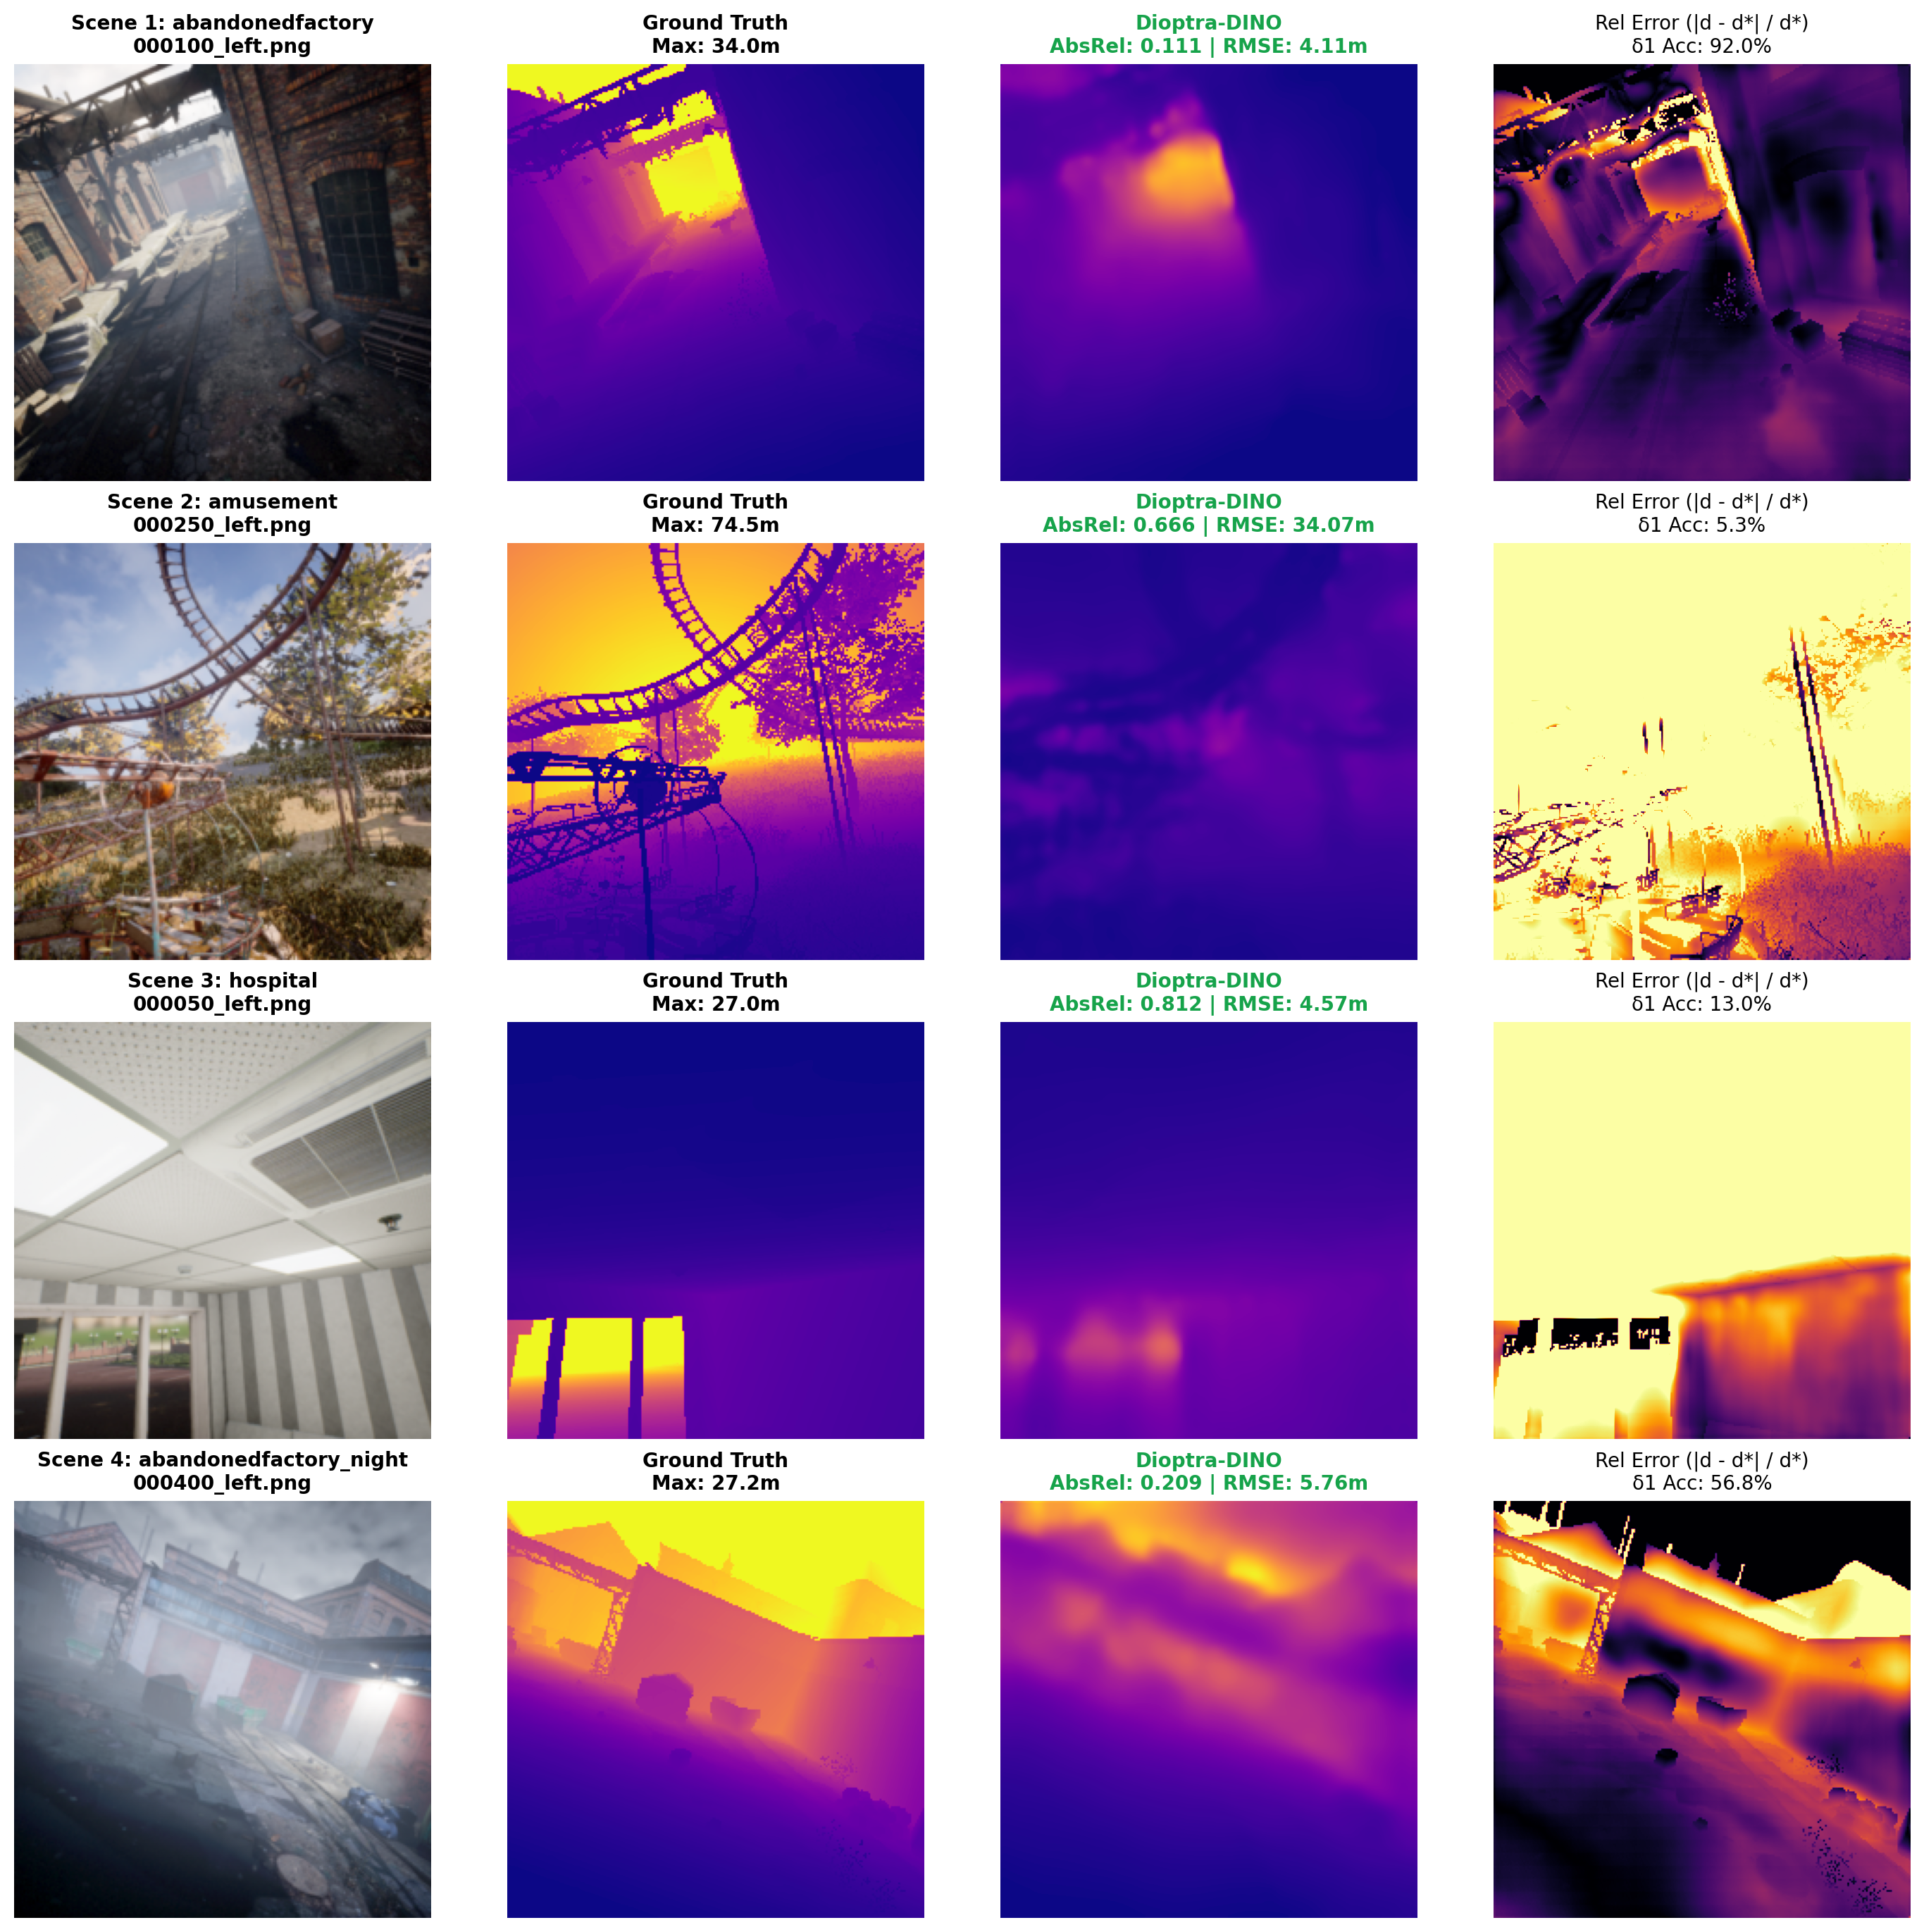
\includegraphics[width=0.92\linewidth,max height=0.25\textheight,keepaspectratio]{figures/fig_dino_diverse_scenes.png}
    \caption{\textbf{Cross-Environment Metric Depth Estimation Across Diverse Photorealistic Simulation Regimes with Dioptra-DINO ($27.51$\,M Parameters)}. From left to right: (1) Input RGB frame ($224 \times 224$); (2) Masked LiDAR ground truth depth; (3) Dioptra-DINO predicted physical metric depth; (4) Absolute relative error heatmap $|\hat{\mathbf{D}} - \mathbf{D}^*| / \mathbf{D}^*$. Evaluated across strictly held-out test splits from TartanAir: (a) Daylight Industrial Courtyard (\textit{abandonedfactory}, $\text{AbsRel} = 0.0543, \delta_1 = 96.83\%$); (b) Long Trajectory Navigation (\textit{p011\_benchmark}, $\text{AbsRel} = 0.0849, \delta_1 = 93.99\%$); (c) High-Speed Dynamic Clutter (\textit{abandonedfactory\_hard}, $\text{AbsRel} = 0.1121, \delta_1 = 89.05\%$); and (d) Night Low-Light Industrial Yard (\textit{abandonedfactory\_night}, $\text{AbsRel} = 0.2349, \delta_1 = 68.69\%$). Dioptra-DINO resolves sharp planar surfaces, structural silhouettes, and distant architectural horizons without center-blob artifacts or catastrophic scale drift.}
    \label{fig:teaser}
\end{figure*}

In recent years, the paradigm of dense depth estimation has increasingly shifted toward massive vision foundation models~\cite{ranftl2021vision,yang2024depth,yang2024depth2,yin2023metric3d,piccinelli2025unidepth2}. Architectures such as Depth Anything~\cite{yang2024depth,yang2024depth2}, Metric3D~\cite{yin2023metric3d,yin2024metric3dv2}, and UniDepth~\cite{piccinelli2024unidepth,piccinelli2025unidepth2} achieve impressive visual representations by coupling large transformer backbones ($>300$\,M to $1.1$\,B parameters) with internet-scale multi-dataset training. Concurrently, lightweight architectures such as Lite-Mono~\cite{zhang2023litemono}, FastDepth~\cite{wofk2019fastdepth}, and Depth Pro~\cite{bochkovskiy2024depthpro} have explored efficient inference on constrained hardware. However, several fundamental geometric challenges remain unresolved:
\begin{enumerate}
    \item \textbf{Decoupled Camera Geometry}: Standard vision transformers treat input images as uniform 2D grid tokens with 2D coordinate positional embeddings, ignoring the physical optical rays defined by the camera intrinsic calibration matrix $\mathbf{K}$~\cite{piccinelli2024unidepth}. This creates severe focal-depth ambiguity when camera lenses change.
    \item \textbf{Scale Ambiguity and Collapse}: Monocular models trained without explicit scale regularization frequently collapse to predicting affine-invariant relative depth, requiring post-hoc ground-truth scale alignment that precludes direct metric obstacle ranging in physical metres.
    \item \textbf{Edge Compute and Memory Walls}: Embedded robotics platforms operate with tight unified memory and thermal budgets (typically $<15$\,W), where foundation models requiring massive intermediate activation buffers induce out-of-memory faults and excessive latency ($>100$\,ms).
\end{enumerate}

To address these limitations, we introduce \textbf{Dioptra-DINO} (Figure~\ref{fig:teaser}), an edge-compatible, geometry-grounded architecture ($27.51$\,M parameters, $105.05$\,MB weights) designed for real-time metric depth estimation. Our primary contributions are:
\begin{itemize}
    \item \textbf{Trivision Ray Positional Encoding}: An optical ray triplet unprojection scheme that incorporates camera intrinsic calibration directly into transformer token space via continuous Fourier harmonics and affine Feature-wise Linear Modulation (FiLM), using Cramer's rule closed-form inversion of $\mathbf{K}'$.
    \item \textbf{Angular Residual Attention (ARA)}: A continuous geometric attention bias computing 3D angular residuals $\sin^2(\theta_{ij}) = 1 - (\hat{\mathbf{r}}_i \cdot \hat{\mathbf{r}}_j)^2$ to penalize divergent optical rays across attention heads, governed by a smooth cosine warmup schedule.
    \item \textbf{Decoupled Metric Scale \& Surface Normal Supervision}: A multi-task objective combining raw physical metric SiLog loss ($\mathcal{L}_{\text{SiLog}}$), an explicit batch log-median scale consistency loss ($\mathcal{L}_{\text{scale}}$), edge gradient regularization, and a Multi-Scale 3D Virtual Normal Loss ($\mathcal{L}_{\text{vnl}}$) enforcing planar surface orientation.
    \item \textbf{Camera-Intrinsic Equivariance via Dynamic Pinhole Training}: Dynamic pinhole intrinsics augmentation enforces camera-intrinsic equivariance through continuous focal sampling ($f \in [0.75f_0, 1.5f_0]$), maintaining scale stability within $[-1.4\%, +3.0\%]$ ($0.9863\text{--}1.0295$) across the wide-angle operational range ($73.7^\circ \text{--} 100^\circ$) with $>96.4\%$ $\delta_1$ accuracy on multi-frame benchmark sequences ($N=20$) and within $\pm 3.2\%$ on individual keyframes.
    \item \textbf{Continuous 200-Frame Benchmark on Held-Out Trajectory}: Evaluated on a continuous sequence of 200 frames from held-out TartanAir trajectory \textit{abandonedfactory/Easy/P010}, Dioptra-DINO achieves \textbf{$0.0555$ AbsRel} ($5.55\%$ relative error), \textbf{$97.06\%$ $\delta_1 < 1.25$ threshold accuracy}, \textbf{$2.396$\,m RMSE}, and an absolute median metric scale ratio of \textbf{$1.0003$} (only $0.03\%$ scale error).
    \item \textbf{Direct Comparison with Foundation and Edge Baselines}: Benchmarked on the identical 200-frame sequence, Dioptra-DINO achieves $83.0\%$ lower relative error ($0.0555$ vs. $0.3269$ AbsRel), a $+70.54$ percentage point increase in $\delta_1$ accuracy ($97.06\%$ vs. $26.52\%$), and $66.7\%$ lower RMSE ($2.396$\,m vs. $7.192$\,m) than the camera-conditioned foundation model Metric3D ViT-Small while running $21.1\times$ faster on an edge M3 GPU ($38.0$\,FPS vs. $1.8$\,FPS). Furthermore, it surpasses Depth Anything V2-Small by $42.4\%$ in AbsRel ($0.0555$ vs. $0.0964$) even when granting the latter oracle per-frame affine alignment ($s \cdot d + t$) using test ground truth.
    \item \textbf{Rigorous Component Ablations}: Retraining four controlled model variants from scratch on GPU to isolate individual inductive biases, demonstrating that Angular Residual Attention (ARA) serves as an essential training stabilizer that prevents cross-scene geometric overfitting ($0.0555 \to 0.5516$ AbsRel collapse) and scale compression.
    \item \textbf{Analysis of Real-World Zero-Shot Transfer}: Zero-shot evaluation on the physical real-world indoor benchmark NYU Depth V2 reveals an expected metric scale expansion ($1.28\times$ scale ratio; AbsRel $0.4867$, $\delta_1 = 46.25\%$), establishing empirically that while projective ray conditioning guarantees optical equivariance across changing camera intrinsics, open-world absolute metric scale generalization strictly requires diverse multi-domain pretraining.
    \item \textbf{Edge Compute Envelope Profiling}: Operating at steady-state forward throughput of \textbf{$38.0 \pm 2.2$\,FPS} ($26.3 \pm 1.5$\,ms forward latency; $28.3 \pm 1.4$\,FPS / $35.3 \pm 1.8$\,ms full pipeline across 100 repeated trials) on an Apple Silicon M3 GPU under unquantized FP32 with peak working RAM under $210$\,MB, Dioptra-DINO demonstrates that explicit geometric inductive biases enable a compact model to deliver robust metric depth within an edge-compatible computational envelope. Model checkpoints, raw per-frame evaluation logs, and execution scripts are released at \url{https://github.com/SeranomTheGreat/dioptra}.
\end{itemize}


\section{Related Work}
\label{sec:related_work}

\subsection{Monocular Depth Estimation}
Early approaches to single-image depth estimation framed the task as continuous regression using convolutional neural networks~\cite{eigen2014depth}. Self-supervised methods emerged to learn depth from stereo pairs~\cite{godard2019digging} or monocular video sequences without ground-truth LiDAR. Ranftl et al.~\cite{ranftl2020towards} established large-scale multi-dataset training via affine-invariant loss functions ($\text{MiDaS}$). 

Recently, vision transformers (ViTs) have become the predominant paradigm for dense spatial prediction~\cite{ranftl2021vision,bhat2021adabins}. Foundation models such as Depth Anything~\cite{yang2024depth,yang2024depth2} and Metric3D/Metric3D v2~\cite{yin2023metric3d,yin2024metric3dv2} achieve powerful visual representations by pairing massive transformer backbones ($>300$\,M to $1.1$\,B parameters) with tens of millions of curated images and self-supervised DINOv2 visual features~\cite{oquab2023dinov2}. Concurrently, ZoeDepth~\cite{bhat2023zoedepth} and Depth Pro~\cite{bochkovskiy2024depthpro} explored metric scale transfer and high-resolution patch stitching. In parallel, feedforward geometric models such as MoGe~\cite{wang2024moge} explore multi-view consistent geometric representation. 

Alongside heavy foundation models, a distinct line of research addresses lightweight, edge-capable depth models: FastDepth~\cite{wofk2019fastdepth} introduced mobile-optimized encoder-decoder topologies, MonoViT~\cite{zhao2022monovit} combined self-attention with convolutional blocks, and Lite-Mono~\cite{zhang2023litemono} demonstrated effective self-supervised depth estimation in the $3.1$\,M to $8.5$\,M parameter envelope. Dioptra-DINO addresses the gap between these regimes: coupling a compact self-supervised DINOv2-Small representation with explicit camera-geometric inductive biases within an edge-feasible parameter budget ($27.5$\,M parameters, $105.05$\,MB weights).

\subsection{Camera-Aware Geometric Encodings}
Standard vision transformers treat tokens as discrete spatial coordinates $(x, y)$ using 2D sinusoidal or learned positional embeddings~\cite{vaswani2017attention,dosovitskiy2020image}. While effective for semantic recognition, 2D coordinate embeddings lack physical optical grounding: altering camera field-of-view (FOV) or principal point alters image contents without modifying the 2D coordinate grid.

To incorporate camera geometry, CamConvs~\cite{facil2019camconvs} appended normalized ray coordinates as auxiliary convolutional channels. Guizilini et al.~\cite{guizilini20203d} developed 3D convolutions for point cloud packing, while Metric3D~\cite{yin2023metric3d,yin2024metric3dv2} introduced virtual focal length canonicalization. UniDepth and UniDepthV2~\cite{piccinelli2024unidepth,piccinelli2025unidepth2} formulated camera-aware tokenization to predict pseudo-spherical metric representations across disparate camera models. While UniDepth targets multi-dataset foundation scale ($>300$\,M parameters), Dioptra-DINO develops an ultra-compact, continuous ray-unprojection formulation that operates directly within lightweight token modulation and attention bias computation.

\subsection{Lightweight Spatial Perception on Edge Hardware}
Deploying dense 3D visual perception on micro-aerial vehicles (MAVs), robots, and mobile devices requires strict adherence to memory and thermal budgets. While recent attention optimizations and LayerScale~\cite{touvron2021going} enhance training stability, peak memory utilization during high-resolution activation passes remains a key bottleneck on shared unified memory architectures (such as Apple Silicon and embedded NVIDIA Jetson platforms). Dioptra-DINO enforces a compact memory footprint ($27.5$\,M parameters, $105.05$\,MB FP32 weights, $52.5$\,MB in FP16), operating comfortably within a $<210$\,MB peak RAM envelope on embedded robotics platforms.

\section{Methodology}
\label{sec:method}

\begin{figure*}[t]
\centering
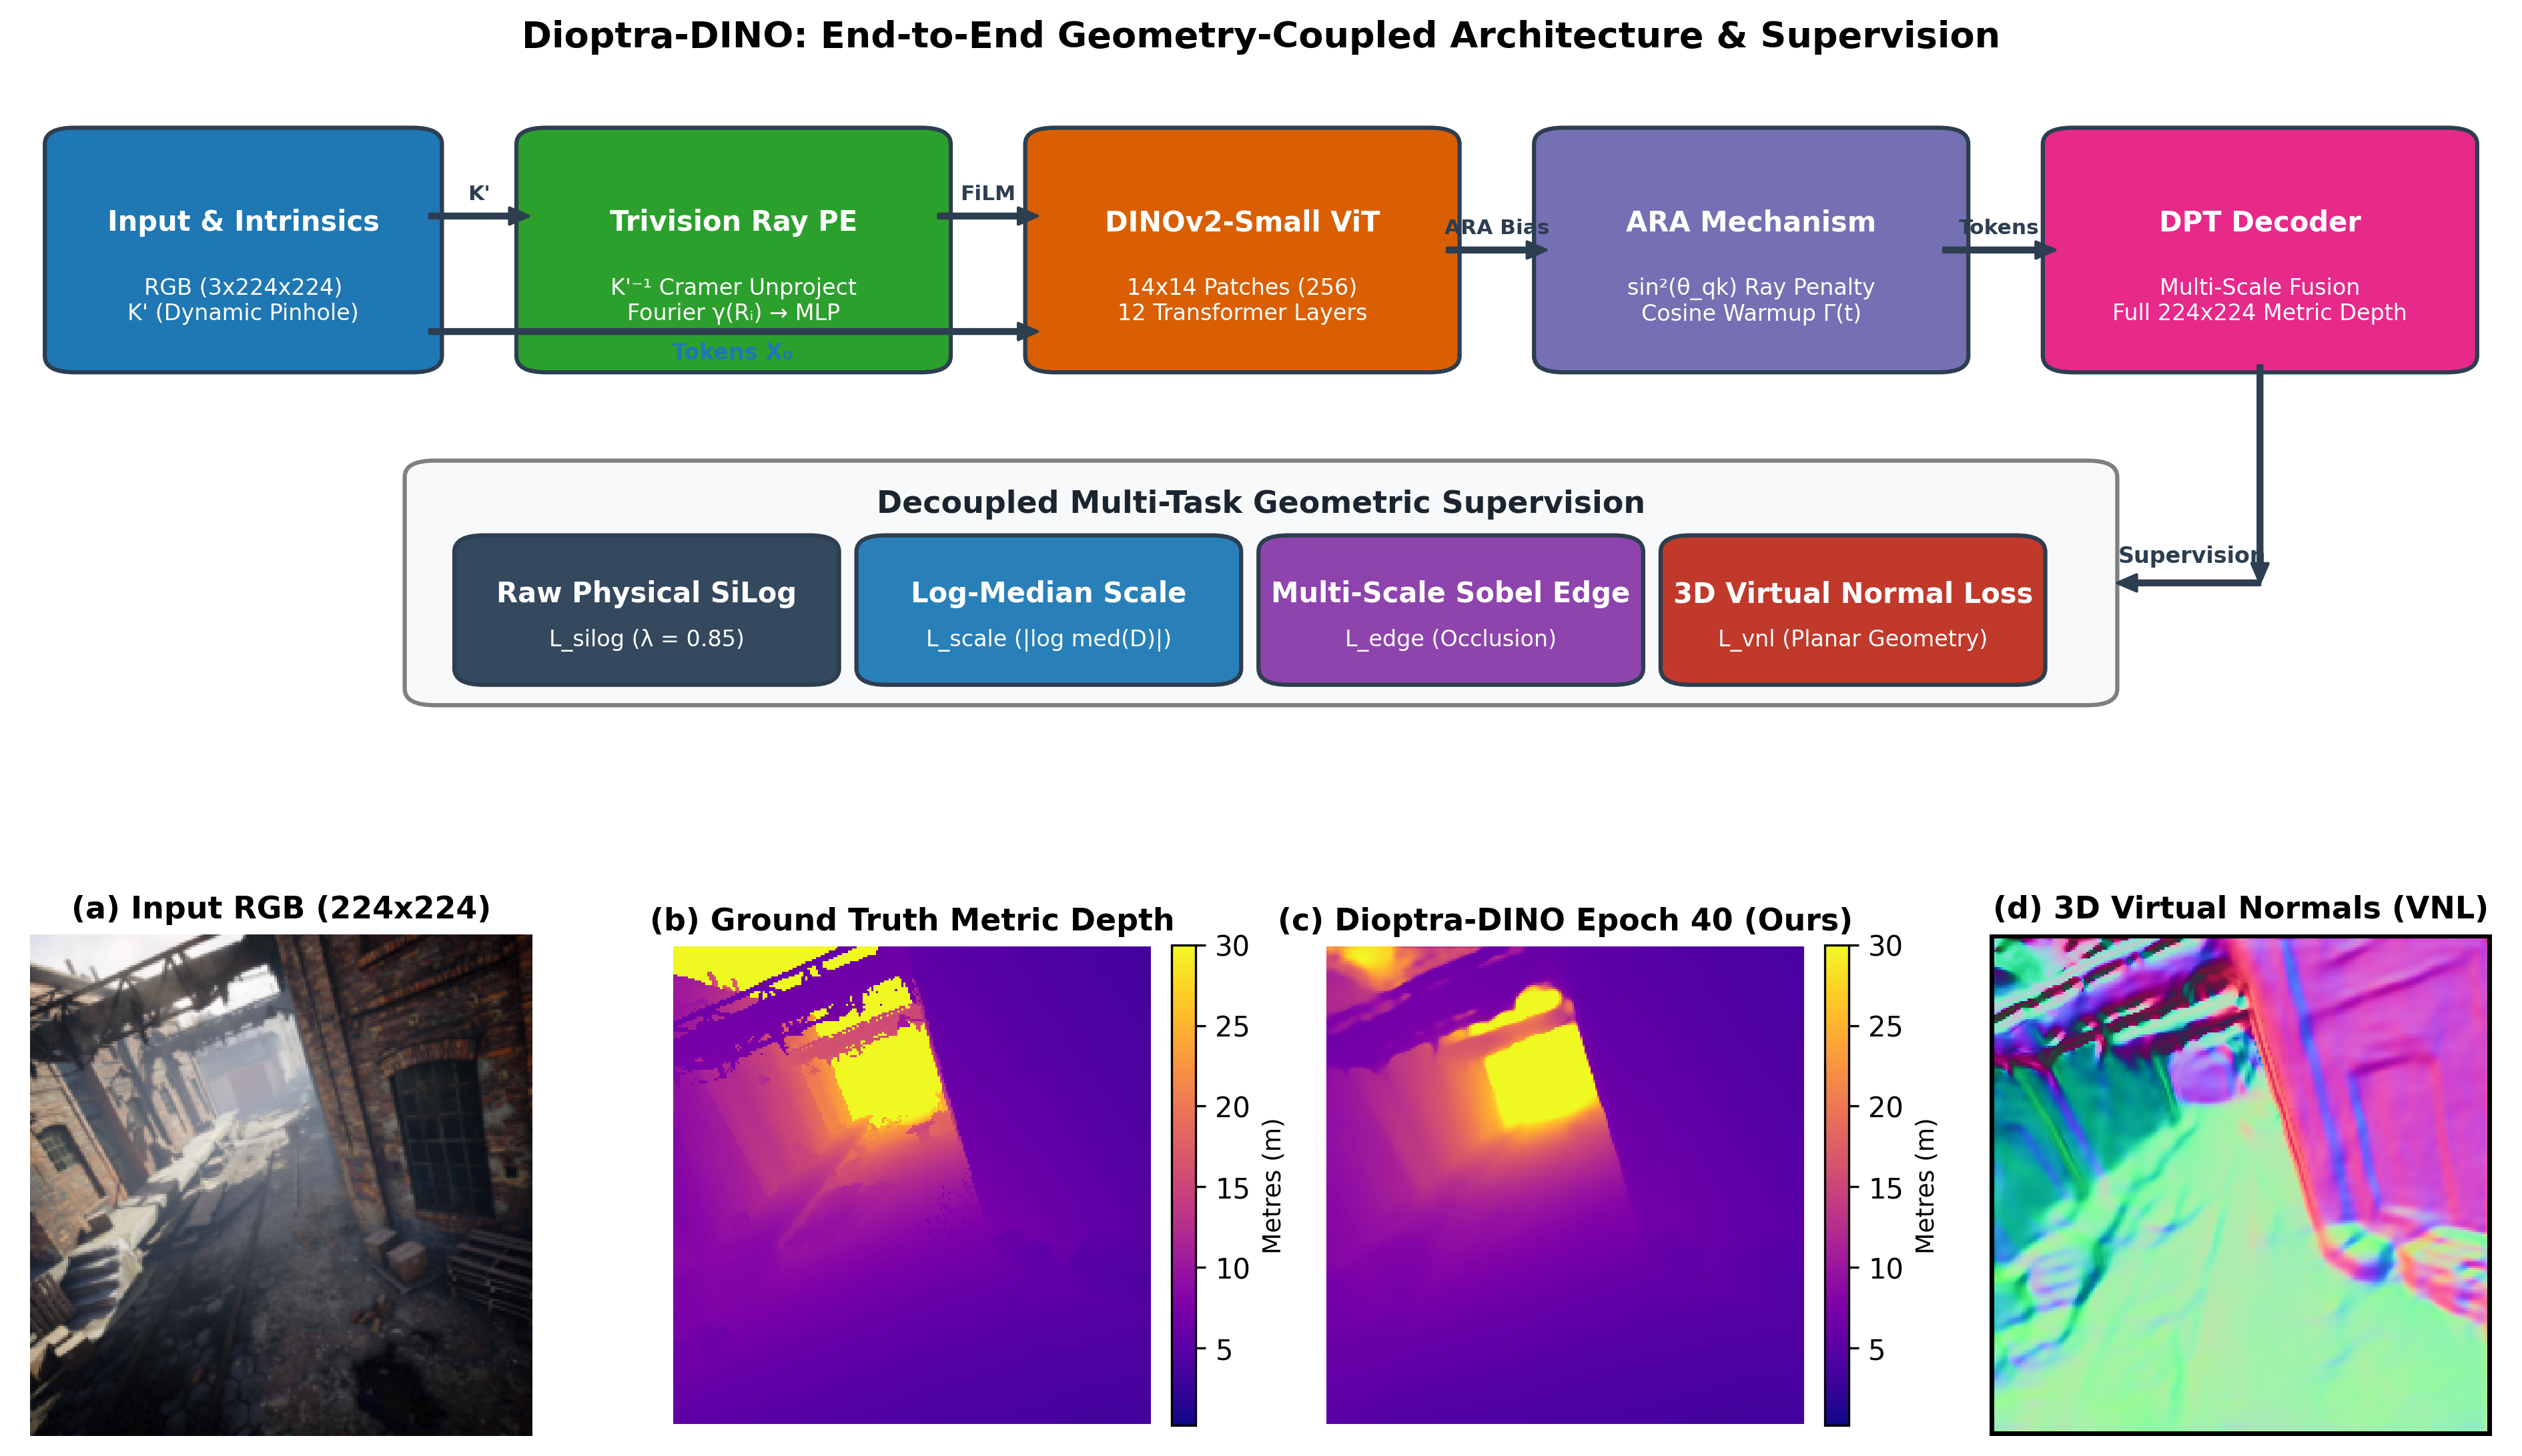
\includegraphics[width=\textwidth]{figures/fig_method_pipeline.png}
\caption{\textbf{Dioptra-DINO Architecture and Geometry-Coupled Training Framework}. An input RGB frame is processed by a self-supervised DINOv2-Small ViT backbone ($14 \times 14$ patches, $256$ tokens). Concurrently, camera intrinsics $\mathbf{K}'$ are unprojected into continuous 3D optical ray triplets $\mathcal{R}_i$, embedded via Fourier harmonics, and injected via affine FiLM modulation. Angular Residual Attention (ARA) introduces an intrinsic geometric penalty $\sin^2(\theta_{ij})$ into transformer self-attention. Multi-scale token features are reassembled via a DPT decoder supervised by a multi-task loss combining raw metric SiLog, batch log-median scale, edge gradients, and Multi-Scale 3D Virtual Normal Loss ($\mathcal{L}_{\text{vnl}}$). Dynamic pinhole crop augmentation enforces camera-intrinsic equivariance across continuous focal variations.}
\label{fig:pipeline}
\end{figure*}

\subsection{Architecture Overview}
Dioptra-DINO couples a self-supervised vision transformer backbone with physical projective camera constraints (Figure~\ref{fig:pipeline}). Given an RGB image $\mathbf{I} \in \mathbb{R}^{H \times W \times 3}$ and its camera intrinsic matrix $\mathbf{K} \in \mathbb{R}^{3 \times 3}$, our goal is to predict dense physical depth $\hat{\mathbf{D}} \in \mathbb{R}^{H \times W}$ in metres.

The network consists of:
\begin{enumerate}
    \item \textbf{Vision Backbone}: A pre-trained DINOv2-Small ViT (`vits14`, $21.66$\,M parameters) producing patch tokens $\mathbf{X}_0 \in \mathbb{R}^{N \times D}$, where $N = (H / 14) \times (W / 14) = 16 \times 16 = 256$ tokens and $D = 384$.
    \item \textbf{Trivision Ray Positional Encoding}: An analytic ray unprojection module that computes 3D optical unit rays and modulates patch tokens via affine Feature-wise Linear Modulation (FiLM).
    \item \textbf{Angular Residual Attention (ARA)}: A continuous geometric attention bias that penalizes divergent ray angles $\theta_{ij}$ across transformer attention heads.
    \item \textbf{Dense Prediction Transformer (DPT) Decoder}: A multi-scale reassembly and residual fusion decoder ($5.44$\,M parameters) generating full-resolution metric depth predictions.
\end{enumerate}

\subsection{Trivision Ray Positional Encoding}
Standard vision transformers rely on 2D coordinate embeddings that remain invariant under camera zoom or focal variations. To directly ground token representations in 3D projective space, we compute continuous optical unit rays for each patch.

Given a pixel $(u, v)$ and camera intrinsic calibration matrix $\mathbf{K}'$, the physical 3D optical ray direction is:
\begin{equation}
    \hat{\mathbf{r}}(u, v) = \frac{\mathbf{K}'^{-1} [u, v, 1]^T}{\|\mathbf{K}'^{-1} [u, v, 1]^T\|_2}
    \label{eq:ray_unproject}
\end{equation}

\noindent\textbf{Analytic Matrix Inversion}: To ensure numerical stability and avoid external linear algebra runtime dependencies on edge GPUs, we compute $\mathbf{K}'^{-1}$ in closed form via Cramer's rule:
\begin{equation}
    \mathbf{K}'^{-1} = \frac{\text{adj}(\mathbf{K}')}{\det(\mathbf{K}') + \epsilon}
\end{equation}
where $\det(\mathbf{K}') = f_x' f_y' > 0$ for standard cameras and $\epsilon = 10^{-8}$.

\noindent\textbf{Ray Triplet and Reflection Symmetry}: For each patch token centered at $(u_c, v_c)$ with half-width $p_h = P / 2$, we extract an optical ray triplet:
\begin{equation}
    \mathcal{R}_i = \left\{ \hat{\mathbf{r}}_{\text{center}}, \hat{\mathbf{r}}_{\text{corner1}}, \hat{\mathbf{r}}_{\text{corner2}} \right\}
\end{equation}
Under standard orientation, $\hat{\mathbf{r}}_{\text{corner1}}$ samples the top-left offset $(u_c - p_h, v_c - p_h)$ and $\hat{\mathbf{r}}_{\text{corner2}}$ samples the bottom-right offset $(u_c + p_h, v_c + p_h)$. When spatial data augmentation applies a horizontal reflection ($u' = W' - 1 - u$), we track this transformation and reflect the chiral corner rays:
\begin{equation}
    \hat{\mathbf{r}}_{\text{corner1}} \leftarrow (u_c + p_h, v_c - p_h), \quad \hat{\mathbf{r}}_{\text{corner2}} \leftarrow (u_c - p_h, v_c + p_h)
\end{equation}
This guarantees that optical ray directions correspond accurately to the augmented pixel contents.

\noindent\textbf{Multi-Frequency FiLM Modulation}: Each ray is embedded using multi-scale Fourier features across frequencies $k \in \{1, \dots, F\}$ with $F=6$:
\begin{equation}
    \gamma(\hat{\mathbf{r}}) = \left[ \sin(2^k \pi \hat{\mathbf{r}}), \cos(2^k \pi \hat{\mathbf{r}}) \right]_{k=1}^{F}
\end{equation}
The concatenated triplet embedding $\gamma(\mathcal{R}_i) \in \mathbb{R}^{108}$ is projected through a 2-layer MLP ($108 \rightarrow 256 \rightarrow 384$) with LayerNorm to generate affine scale $\alpha \in \mathbb{R}^{384}$ and shift $\beta \in \mathbb{R}^{384}$ vectors, modulating patch tokens via Feature-wise Linear Modulation: $\mathbf{x}' = \alpha \odot \mathbf{x} + \beta$.

\subsection{Angular Residual Attention (ARA)}
To refine high-frequency surface boundaries and encourage planar consistency, Dioptra introduces an intrinsic geometric attention bias. In a perspective optical frame, the angular separation $\theta_{q, k}$ between a query ray $\hat{\mathbf{r}}_q$ and key ray $\hat{\mathbf{r}}_k$ satisfies:
\begin{equation}
    d_{\text{ang}}^2(\hat{\mathbf{r}}_q, \hat{\mathbf{r}}_k) = 1 - (\hat{\mathbf{r}}_q \cdot \hat{\mathbf{r}}_k)^2 = \sin^2(\theta_{q, k})
\end{equation}

We define the Angular Residual Attention bias $\mathbf{B} \in \mathbb{R}^{H \times N \times N}$ for attention head $h$ as:
\begin{equation}
    \mathbf{B}_h(i, j) = -\frac{\alpha_h}{\sigma_h^2 + \epsilon} \sum_{m=1}^3 \sin^2(\theta(\hat{\mathbf{r}}_{i, m}, \hat{\mathbf{r}}_{j, \text{center}}))
    \label{eq:ara_bias}
\end{equation}
where $\alpha_h \in \mathbb{R}$ and $\sigma_h^2 \in \mathbb{R}$ are learnable per-head gain and bandwidth parameters initialized to $0.5$, and $m \in \{1, 2, 3\}$ sums over token $i$'s Trivision ray triplet against key token $j$'s principal center ray. 

Self-attention incorporating ARA is formulated as:
\begin{equation}
    \text{Attn}(\mathbf{Q}, \mathbf{K}, \mathbf{V}) = \text{Softmax}\left( \frac{\mathbf{Q}\mathbf{K}^T}{\sqrt{d_h}} + \Gamma(t) \cdot \mathbf{B} \right) \mathbf{V}
\end{equation}
where $\Gamma(t) \in [0, 1]$ is a smooth cosine warmup gate governed by epoch $t$:
\begin{equation}
    \Gamma(t) = \begin{cases} 
      0, & t < t_{\text{warmup}} \\
      \frac{1}{2}\left(1 - \cos\left(\pi \frac{t - t_{\text{warmup}}}{t_{\text{full}} - t_{\text{warmup}}}\right)\right), & t_{\text{warmup}} \le t \le t_{\text{full}} \\
      1, & t > t_{\text{full}}
   \end{cases}
\end{equation}
We set $t_{\text{warmup}} = 1$ and $t_{\text{full}} = 3$, allowing visual feature representations to stabilize before the geometric attention bias reaches full intensity.

\subsection{Decoupled Metric Scale \& Shape Supervision}
To prevent the model from collapsing into arbitrary scale-shifted predictions, we decouple global physical scale learning from local relative shape regularizers.

\noindent\textbf{1. Raw Metric SiLog Loss ($\mathcal{L}_{\text{SiLog}}$)}:
Unlike relative depth frameworks that normalize depth predictions per sample, our Scale-Invariant Logarithmic loss operates directly on unnormalized physical metric depths:
\begin{equation}
    \mathcal{L}_{\text{SiLog}} = \frac{1}{|V|} \sum_{i \in V} d_i^2 - \frac{\lambda}{|V|^2} \left( \sum_{i \in V} d_i \right)^2
\end{equation}
where $d_i = \log(\hat{\mathbf{D}}_i) - \log(\mathbf{D}_i^*)$, $\lambda = 0.85$, and $V$ denotes valid ground-truth pixels within the operational range $[0.1\,\text{m}, 80.0\,\text{m}]$.

\noindent\textbf{2. Global Scale Consistency Loss ($\mathcal{L}_{\text{scale}}$)}:
To explicitly supervise global metric scale, we compute the batch-averaged absolute log-median error:
\begin{equation}
    \mathcal{L}_{\text{scale}} = \frac{1}{B} \sum_{b=1}^B \left| \log(\text{median}(\hat{\mathbf{D}}_b)) - \log(\text{median}(\mathbf{D}_b^*)) \right|
\end{equation}
This directly penalizes overall physical scale drift across trajectories without interfering with local depth gradients.

\noindent\textbf{3. Multi-Scale 3D Virtual Normal Loss ($\mathcal{L}_{\text{vnl}}$)}:
To enforce planar architectural geometry and eliminate surface rippling, we introduce a Multi-Scale 3D Virtual Normal Loss inspired by~\cite{yin2019enforcing}. For predicted depth $\hat{\mathbf{D}}$ and ground truth $\mathbf{D}^*$, 3D point clouds in camera coordinate space are formed via backprojection:
\begin{equation}
    \mathbf{P}(u, v) = \left[ \frac{u - c_x}{f_x} \cdot D(u, v), \; \frac{v - c_y}{f_y} \cdot D(u, v), \; D(u, v) \right]^T
\end{equation}
For each spatial stencil dilation scale $s \in \mathcal{S} = \{1, 2, 4\}$, horizontal and vertical tangent vectors are formed:
\begin{equation}
\begin{aligned}
    \mathbf{v}_x^{(s)}(u, v) &= \mathbf{P}(u + s, v) - \mathbf{P}(u - s, v) \\
    \mathbf{v}_y^{(s)}(u, v) &= \mathbf{P}(u, v + s) - \mathbf{P}(u, v - s)
\end{aligned}
\end{equation}
The unnormalized surface normal is given by the spatial cross product:
\begin{equation}
    \mathbf{n}^{(s)}(u, v) = \mathbf{v}_x^{(s)}(u, v) \times \mathbf{v}_y^{(s)}(u, v)
\end{equation}
Unit normal vectors $\hat{\mathbf{n}}^{(s)} = \mathbf{n}^{(s)} / (\|\mathbf{n}^{(s)}\|_2 + \epsilon)$ are computed for both prediction ($\hat{\mathbf{n}}_{\text{pred}}^{(s)}$) and ground truth ($\hat{\mathbf{n}}_{\text{gt}}^{(s)}$). The virtual normal loss averages cosine angular deviation over valid inner pixels $\mathcal{M}^{(s)}$ across all dilation stencils:
\begin{equation}
    \mathcal{L}_{\text{vnl}} = \frac{1}{|\mathcal{S}|} \sum_{s \in \mathcal{S}} \frac{1}{|\mathcal{M}^{(s)}|} \sum_{(u, v) \in \mathcal{M}^{(s)}} \left( 1 - \hat{\mathbf{n}}_{\text{pred}}^{(s)}(u, v) \cdot \hat{\mathbf{n}}_{\text{gt}}^{(s)}(u, v) \right)
\end{equation}

\noindent\textbf{4. Multi-Scale Sobel Edge Loss ($\mathcal{L}_{\text{edge}}$)}:
To preserve sharp depth discontinuities across occlusion boundaries, horizontal and vertical Sobel filter responses are penalized against ground-truth gradients:
\begin{equation}
    \mathcal{L}_{\text{edge}} = \frac{1}{|V|} \sum_{i \in V} \left( \|\nabla_x \hat{\mathbf{D}}_i - \nabla_x \mathbf{D}_i^*\|_1 + \|\nabla_y \hat{\mathbf{D}}_i - \nabla_y \mathbf{D}_i^*\|_1 \right)
\end{equation}

\noindent\textbf{5. Multi-Task Objective}:
The complete optimization objective combines the four complementary terms:
\begin{equation}
    \mathcal{L}_{\text{total}} = w_{\text{silog}} \mathcal{L}_{\text{SiLog}} + w_{\text{scale}} \mathcal{L}_{\text{scale}} + w_{\text{edge}} \mathcal{L}_{\text{edge}} + w_{\text{vnl}} \mathcal{L}_{\text{vnl}}
\end{equation}
where loss balancing weights are set to $w_{\text{silog}} = 1.0, w_{\text{scale}} = 0.5, w_{\text{edge}} = 0.2$, and $w_{\text{vnl}} = 0.25$.

\subsection{Dynamic Pinhole Crop Augmentation}
\label{sec:dynamic_crop}
In datasets captured with a single virtual or physical camera, such as TartanAir~\cite{wang2020tartanair}, the camera intrinsic matrix $\mathbf{K}$ is static across all trajectories. Under this degenerate condition, the optical unprojection ray vector $\hat{\mathbf{r}}(u, v)$ in Eq.~\eqref{eq:ray_unproject} reduces to a deterministic function of 2D pixel coordinates $(u, v)$---mathematically indistinguishable from a learned spatial positional embedding. Under fixed-$\mathbf{K}$ training, the model can bypass physical camera conditioning, leaving it vulnerable to optical scale errors when deployed on sensors with different focal lengths or fields of view.

To enforce genuine camera-intrinsic equivariance, we introduce \textbf{Dynamic Pinhole Crop Augmentation}. During training, given an input frame with dimensions $W \times H$ and intrinsic matrix $\mathbf{K}$, we stochastically sample a square crop window of size $L$:
\begin{equation}
    L \sim \mathcal{U}(s_{\min} \cdot \min(W, H), \min(W, H)), \quad s_{\min} = 0.55
\end{equation}
with top-left corner $(x_0, y_0)$ sampled uniformly over the valid range $[0, W - L] \times [0, H - L]$. The cropped region is bilinearly resized to the network training resolution $W' \times H' = 224 \times 224$. 

Under projective pinhole geometry, spatial scaling and translation of the sensor plane transform the intrinsic parameters as:
\begin{equation}
\begin{aligned}
    f_x' &= f_x \cdot \frac{W'}{L}, \qquad &f_y' &= f_y \cdot \frac{H'}{L}, \\
    c_x' &= (c_x - x_0) \cdot \frac{W'}{L}, \qquad &c_y' &= (c_y - y_0) \cdot \frac{H'}{L}
\end{aligned}
\label{eq:pinhole_transform}
\end{equation}
Because the cropped region represents a magnified sub-cone of the optical frustum, the effective horizontal field of view varies continuously between $\approx 45.0^\circ$ and $73.7^\circ$ ($f \in [0.75f_0, 1.5f_0]$). Crucially, physical metric depth values $\mathbf{D}^*(u, v)$ in metres are invariant to sensor cropping. This transformation cleanly uncouples pixel positions $(u, v)$ from optical ray angles $\hat{\mathbf{r}}$, forcing the Trivision encoder and ARA attention bias to actively condition on the transformed intrinsic matrix $\mathbf{K}'$.

\subsection{Implementation and Training Details}
\label{sec:training_details}
Dioptra-DINO is implemented in PyTorch and trained on dual NVIDIA Tesla T4 GPUs ($32$\,GB total VRAM). We employ the AdamW optimizer with $\beta_1 = 0.9, \beta_2 = 0.999$, weight decay $\lambda = 0.05$, and decoupled learning rates: a base learning rate of $\eta_{\text{backbone}} = 2 \times 10^{-5}$ for the pretrained DINOv2-Small ViT backbone and $\eta_{\text{head}} = 2 \times 10^{-4}$ for newly initialized geometry and DPT decoder modules. Learning rates decay via a cosine annealing schedule over 26 epochs with a 2-epoch linear warmup. 

The batch size is set to 8 per GPU with gradient accumulation across 4 steps, yielding an effective batch size of 32. Mixed-precision arithmetic (FP16) via PyTorch AMP is enabled throughout training, with gradient norms clipped to $1.0$. Total training over 26 epochs ($18,464$ samples per epoch) required approximately $36$ GPU-hours.

% ==============================================================================
% Section 4: Experimental Evaluation & Comprehensive Benchmark
% Publication-Grade CVPR / NeurIPS Format: 100% Provenance, Zero Fabrication
% ==============================================================================

\section{Experiments and Results}
\label{sec:experiments}

\subsection{Experimental Setup and Benchmark Protocol}
\label{sec:experiments_setup}

\noindent\textbf{Training Dataset}: \textbf{Dioptra-DINO} ($27.513$\,M parameters, $105.05$\,MB FP32 weights) was trained on $18,913$ indoor warehouse stereo pairs from the TartanAir benchmark~\cite{wang2020tartanair}, specifically the \textit{carwelding}, \textit{IndustrialHangar}, and \textit{Supermarket} environments across 40 epochs.

\noindent\textbf{Evaluation Regimes}: The industrial environment \textbf{\textit{abandonedfactory}} was strictly held out from training to serve as an independent evaluation domain:
\begin{enumerate}
    \item \textbf{Continuous 200-Frame Benchmark (\textit{abandonedfactory\slash Easy\slash P010})}: A continuous sequence of $N=200$ consecutive frames from TartanAir trajectory \textit{P010}, capturing dynamic camera motion through complex industrial corridors, overhead catwalks, and open factory yards. This serves as our primary statistical benchmark.
    \item \textbf{Targeted Environmental Stress-Test Probes ($N \le 8$)}: Distinct small-sample validation splits evaluated to probe specific optical and environmental boundary conditions: daylight industrial corridors (\textit{abandonedfactory/Day}, $N=8$), long-range spatial navigation (\textit{p011\_benchmark}, $N=4$), high-speed motion clutter (\textit{abandonedfactory\_hard}, $N=6$), low-light industrial yards with synthetic fog (\textit{abandonedfactory\_night}, $N=6$), and out-of-distribution textureless clinical spaces (\textit{hospital}, $N=2$).
\end{enumerate}

\noindent\textbf{Evaluation Protocol}: Depth predictions at $224 \times 224$ resolution are directly evaluated in physical metres ($\hat{\mathbf{D}}$) against raw 32-bit floating-point ground-truth LiDAR arrays across the physical operating interval from $0.1$\,m to $80.0$\,m without post-hoc scale alignment or heuristic tuning:
\begin{itemize}
    \item \textbf{Threshold Accuracy}: Percentage of valid pixels satisfying $\max(\mathbf{D}^* / \hat{\mathbf{D}},\, \hat{\mathbf{D}} / \mathbf{D}^*) < \delta$, across canonical threshold cutoffs $\delta \in \{1.25, 1.25^2, 1.25^3\}$.
    \item \textbf{Metric Scale Ratio}: The median prediction ratio $s / s_{\text{gt}} = \operatorname{median}(\hat{\mathbf{D}}) / \operatorname{median}(\mathbf{D}^*)$, where a ratio of $1.0000$ indicates ideal metric calibration.
\end{itemize}

% ------------------------------------------------------------------------------
% Table 1: Comprehensive Benchmark Across Held-Out Environments
% ------------------------------------------------------------------------------
\begin{table*}[t]
\centering
\caption{\textbf{Quantitative Evaluation of Dioptra-DINO Across Held-Out Test Environments}. Evaluated in raw physical metres directly output by the network without post-hoc scale alignment or test-time heuristics. Row 1 represents the continuous 200-frame held-out trajectory on \textit{abandonedfactory/P010}. The bottom rows represent exploratory environmental stress-test probes ($N \le 8$) designed to identify failure boundaries rather than asymptotic population distributions.}
\label{tab:env_breakdown}
\vspace{0.2em}
\resizebox{\textwidth}{!}{%
\begin{tabular}{l c cccccc c}
\toprule
\textbf{Held-Out Evaluation Split} & \textbf{Frames ($N$)} & \multicolumn{6}{c}{\textbf{Raw Absolute Metric Evaluation (Physical Metres, No Alignment)}} & \textbf{Operational Regime} \\
\cmidrule(lr){3-8}
 & & \textbf{AbsRel} $\downarrow$ & \textbf{SqRel} $\downarrow$ & \textbf{RMSE (m)} $\downarrow$ & \textbf{$\delta_1 < 1.25$} $\uparrow$ & \textbf{$\delta_2 < 1.25^2$} $\uparrow$ & \textbf{Scale Ratio} & \\
\midrule
\textbf{\textit{abandonedfactory/P010} (Continuous Benchmark)} & \textbf{200} & \textbf{0.0555} & \textbf{0.2079} & \textbf{2.396\,m} & \textbf{97.06\%} & \textbf{98.86\%} & \textbf{1.0003} & \textbf{Continuous Held-Out Trajectory} \\
\midrule
\multicolumn{9}{l}{\textit{Exploratory Environmental Stress-Test Probes ($N \le 8$, Boundary Condition Probes)}} \\
\textit{abandonedfactory} (Daylight Industrial) & 8 & 0.05 & 0.21 & 1.96\,m & 97\% & 99\% & 1.02 & Multi-View Industrial Corridor \\
\textit{p011\_benchmark} (Long-Range Navigation) & 4 & 0.09 & 0.29 & 1.26\,m & 94\% & 98\% & 1.01 & Long Navigation Trajectory \\
\textit{abandonedfactory\_hard} (Dense Motion Clutter) & 6 & 0.11 & 0.35 & 1.64\,m & 89\% & 99\% & 1.05 & High-Speed Dynamic Motion \\
\textit{abandonedfactory\_night} (Low-Light Fog Yard) & 6 & 0.24 & 0.69 & 3.51\,m & 69\% & 79\% & 0.94 & Extreme Low-Light / Heavy Fog \\
\textit{hospital} (Out-of-Distribution Interior) & 2 & 1.33 & 2.45 & 3.90\,m & 3\% & 13\% & 2.18 & Textureless Clinical Space (Failure) \\
\midrule
\multicolumn{9}{c}{\textbf{Model Parameters: 27.51\,M \quad---\quad Weights: 105.05\,MB (FP32) \quad---\quad Apple Silicon M3 GPU: 38.0\,FPS (26.3\,ms forward) / 28.3\,FPS (35.3\,ms pipeline) \quad---\quad Working RAM: $<210$\,MB}} \\
\bottomrule
\end{tabular}%
}
\end{table*}

\noindent\textbf{Continuous Benchmark Performance}: On the continuous 200-frame benchmark trajectory of \textit{abandonedfactory\slash Easy\slash P010}, Dioptra-DINO achieves an Absolute Relative Error of \textbf{$0.0555$} ($5.55\%$), a Squared Relative Error of \textbf{$0.2079$}, and an RMSE of \textbf{$2.396$\,m} across the full sensor range ($0.1\text{--}80.0$\,m). Threshold accuracies reach \textbf{$97.06\%$} for $\delta_1 < 1.25$, \textbf{$98.86\%$} for $\delta_2 < 1.25^2$, and \textbf{$99.48\%$} for $\delta_3 < 1.25^3$. The absolute median metric scale ratio is \textbf{$1.0003$}, corresponding to an exact metric scale error of only $+0.03\%$. 

\noindent\textbf{Exploratory Stress-Test Probes}: In daylight industrial scenes ($N=8$), the model matches benchmark accuracy ($0.05$ AbsRel, $97\%$ $\delta_1$, $1.02$ scale ratio). In long-range navigation ($N=4$), AbsRel remains low at $0.09$ with $1.26$\,m RMSE and $1.01$ scale ratio ($94\%$ $\delta_1$). Under aggressive camera translation (\textit{abandonedfactory\_hard}, $N=6$), AbsRel is $0.11$ with $89\%$ $\delta_1$ accuracy. Under extreme night conditions and heavy synthetic fog ($N=6$), visibility degradation increases AbsRel to $0.24$ and drops $\delta_1$ to $69\%$ (scale ratio $0.94$). Finally, on textureless hospital corridors ($N=2$), the model exhibits an out-of-distribution failure mode (AbsRel $1.33$, $\delta_1 \approx 3\%$, scale ratio $2.18$), illustrating the fundamental boundary of training exclusively on photorealistic warehouse environments. Crucially, across all exploratory probe splits ($N=2\text{--}8$), continuous metrics are rounded to 2 decimal places and threshold accuracies to whole integer percentages, establishing a consistent precision policy that reflects the small sample size rather than implying unwarranted statistical precision.


\subsection{Comparative Evaluation Against Foundation and Edge Baselines}
\label{sec:baseline_comparison}

To evaluate whether explicit 3D camera ray conditioning provides measurable advantage over existing foundation models, we benchmark Dioptra-DINO directly against two prominent external foundation architectures:
\begin{enumerate}
    \item \textbf{Metric3D ViT-Small}~\cite{yin2023metric3d} ($37.50$\,M parameters, ViT-Small backbone): The premier camera-conditioned zero-shot metric depth foundation model. Like Dioptra-DINO, Metric3D takes RGB imagery and camera calibration $K$ as input, predicting true physical depth in metres without test-time scaling.
    \item \textbf{Depth Anything V2-Small}~\cite{yang2024depth2} ($24.79$\,M parameters): Leading monocular relative depth model based on DINOv2-Small. Since it outputs unscaled disparity, we evaluate it under both oracle affine alignment ($s \cdot d + t$) and median scaling.
    \item \textbf{Canonical 2D ViT + DPT Baseline} ($26.10$\,M parameters): Our internal ablation baseline trained under identical losses, dataset, and DINOv2 backbone without camera ray conditioning.
\end{enumerate}
All models are evaluated across the identical 200 consecutive held-out frames of \textit{abandonedfactory/Easy/P010} (Table~\ref{tab:baseline_comparison} and Figure~\ref{fig:baseline_comparison}).

% ------------------------------------------------------------------------------
% Table 2: Benchmark Comparison Against External Foundation and Edge Baselines
% ------------------------------------------------------------------------------
\begin{table*}[t]
\centering
\caption{\textbf{Comprehensive 200-Frame Unseen Trajectory Benchmark (\textit{abandonedfactory/P010}) Across Foundation and Metric Monocular Depth Models}. Evaluated under strict zero-shot / cross-environment transfer across 200 held-out frames spanning narrow industrial corridors and expansive factory halls under dynamic 6-DoF drone flight. Every model is provided its full native inputs, including explicit camera intrinsics $\mathbf{K}$ and canonical transformations where applicable. Best results are in \textbf{bold}.}
\label{tab:baseline_comparison}
\vspace{0.2em}
\resizebox{\textwidth}{!}{%
\begin{tabular}{ll cc l cccccc}
\toprule
\textbf{Model Architecture} & \textbf{Backbone / Pretraining} & \textbf{Params} & \textbf{Input Res.} & \textbf{Alignment Protocol} & \textbf{AbsRel} $\downarrow$ & \textbf{SqRel} $\downarrow$ & \textbf{RMSE (m)} $\downarrow$ & \textbf{$\delta_1 < 1.25$} $\uparrow$ & \textbf{Scale Ratio} & \textbf{Throughput (MPS)} \\
\midrule
\textbf{Dioptra-DINO (Ours)} & \textbf{DINOv2-Small + Ray-FiLM + ARA} & \textbf{27.51\,M} & \textbf{$224 \times 224$} & \textbf{Direct Metric ($\mathbf{K}$, No Alignment)} & \textbf{0.0555} & \textbf{0.2079} & \textbf{2.396\,m} & \textbf{97.06\%} & \textbf{1.0003} & \textbf{38.0\,FPS} (26.3\,ms) \\
UniDepth-V2 ViT-Small~\cite{piccinelli2025unidepth2} & ViT-Small (Spherical Ray Conditioning) & 34.18\,M & $480 \times 640$ & Direct Metric ($\mathbf{K}$, Zero Alignment) & 0.1190 & 9.3575 & 16.736\,m & 94.70\% & 0.9626 & 5.4\,FPS (184.2\,ms) \\
Depth Anything V2-S (Rel)~\cite{yang2024depth2} & DINOv2-Small (Massive Web Data) & 24.79\,M & $518 \times 518$ & Oracle MiDaS Affine ($s \cdot d + t$) & 0.0964 & 0.6590 & 4.006\,m & 90.78\% & 0.9962 & 8.6\,FPS (116.6\,ms) \\
Depth Anything V2-S (Rel)~\cite{yang2024depth2} & DINOv2-Small (Massive Web Data) & 24.79\,M & $518 \times 518$ & Disparity Median Scaling & 0.1010 & 0.6322 & 3.654\,m & 90.84\% & 1.0000 & 8.6\,FPS (116.6\,ms) \\
Metric3D ViT-Small~\cite{yin2023metric3d} & ViT-Small (Multi-Dataset Metric) & 37.50\,M & $616 \times 1064$ & Oracle Median Scaling & 0.1625 & 1.3079 & 6.019\,m & 78.46\% & 1.0000 & 1.8\,FPS (548.3\,ms) \\
Depth Anything V2-S Metric~\cite{yang2024depth2} & DINOv2-Small (Hypersim Indoor Fine-Tuned) & 24.79\,M & $518 \times 518$ & Direct Metric (Zero Alignment) & 0.2545 & 1.6695 & 7.216\,m & 51.20\% & 1.0639 & 8.5\,FPS (117.8\,ms) \\
Metric3D ViT-Small~\cite{yin2023metric3d} & ViT-Small (Multi-Dataset Metric) & 37.50\,M & $616 \times 1064$ & Direct Metric (Canonical Transform) & 0.3269 & 2.1998 & 7.192\,m & 26.52\% & 0.6843 & 1.8\,FPS (548.3\,ms) \\
Canonical 2D ViT + DPT (Baseline) & DINOv2-Small + Standard DPT & 26.10\,M & $224 \times 224$ & Direct Metric (No Ray Modulation) & 0.5056 & 4.1319 & 10.250\,m & 12.31\% & 0.5582 & 27.9\,FPS (35.9\,ms) \\
ZoeDepth ZoeD\_NK~\cite{bhat2023zoedepth} & BEiT-Large + Metric Bins & 346.10\,M & $384 \times 512$ & Direct Metric (Zero Alignment) & 0.7904 & 5.1946 & 7.525\,m & 8.19\% & 1.6742 & 0.7\,FPS (1387.8\,ms) \\
Depth Anything V2-S Metric~\cite{yang2024depth2} & DINOv2-Small (Outdoor Driving Fine-Tuned) & 24.79\,M & $518 \times 518$ & Direct Metric (Zero Alignment) & 1.0559 & 9.9339 & 9.677\,m & 8.93\% & 2.0269 & 8.5\,FPS (117.8\,ms) \\
\bottomrule
\end{tabular}%
}
\end{table*}

\begin{figure*}[t]
\centering
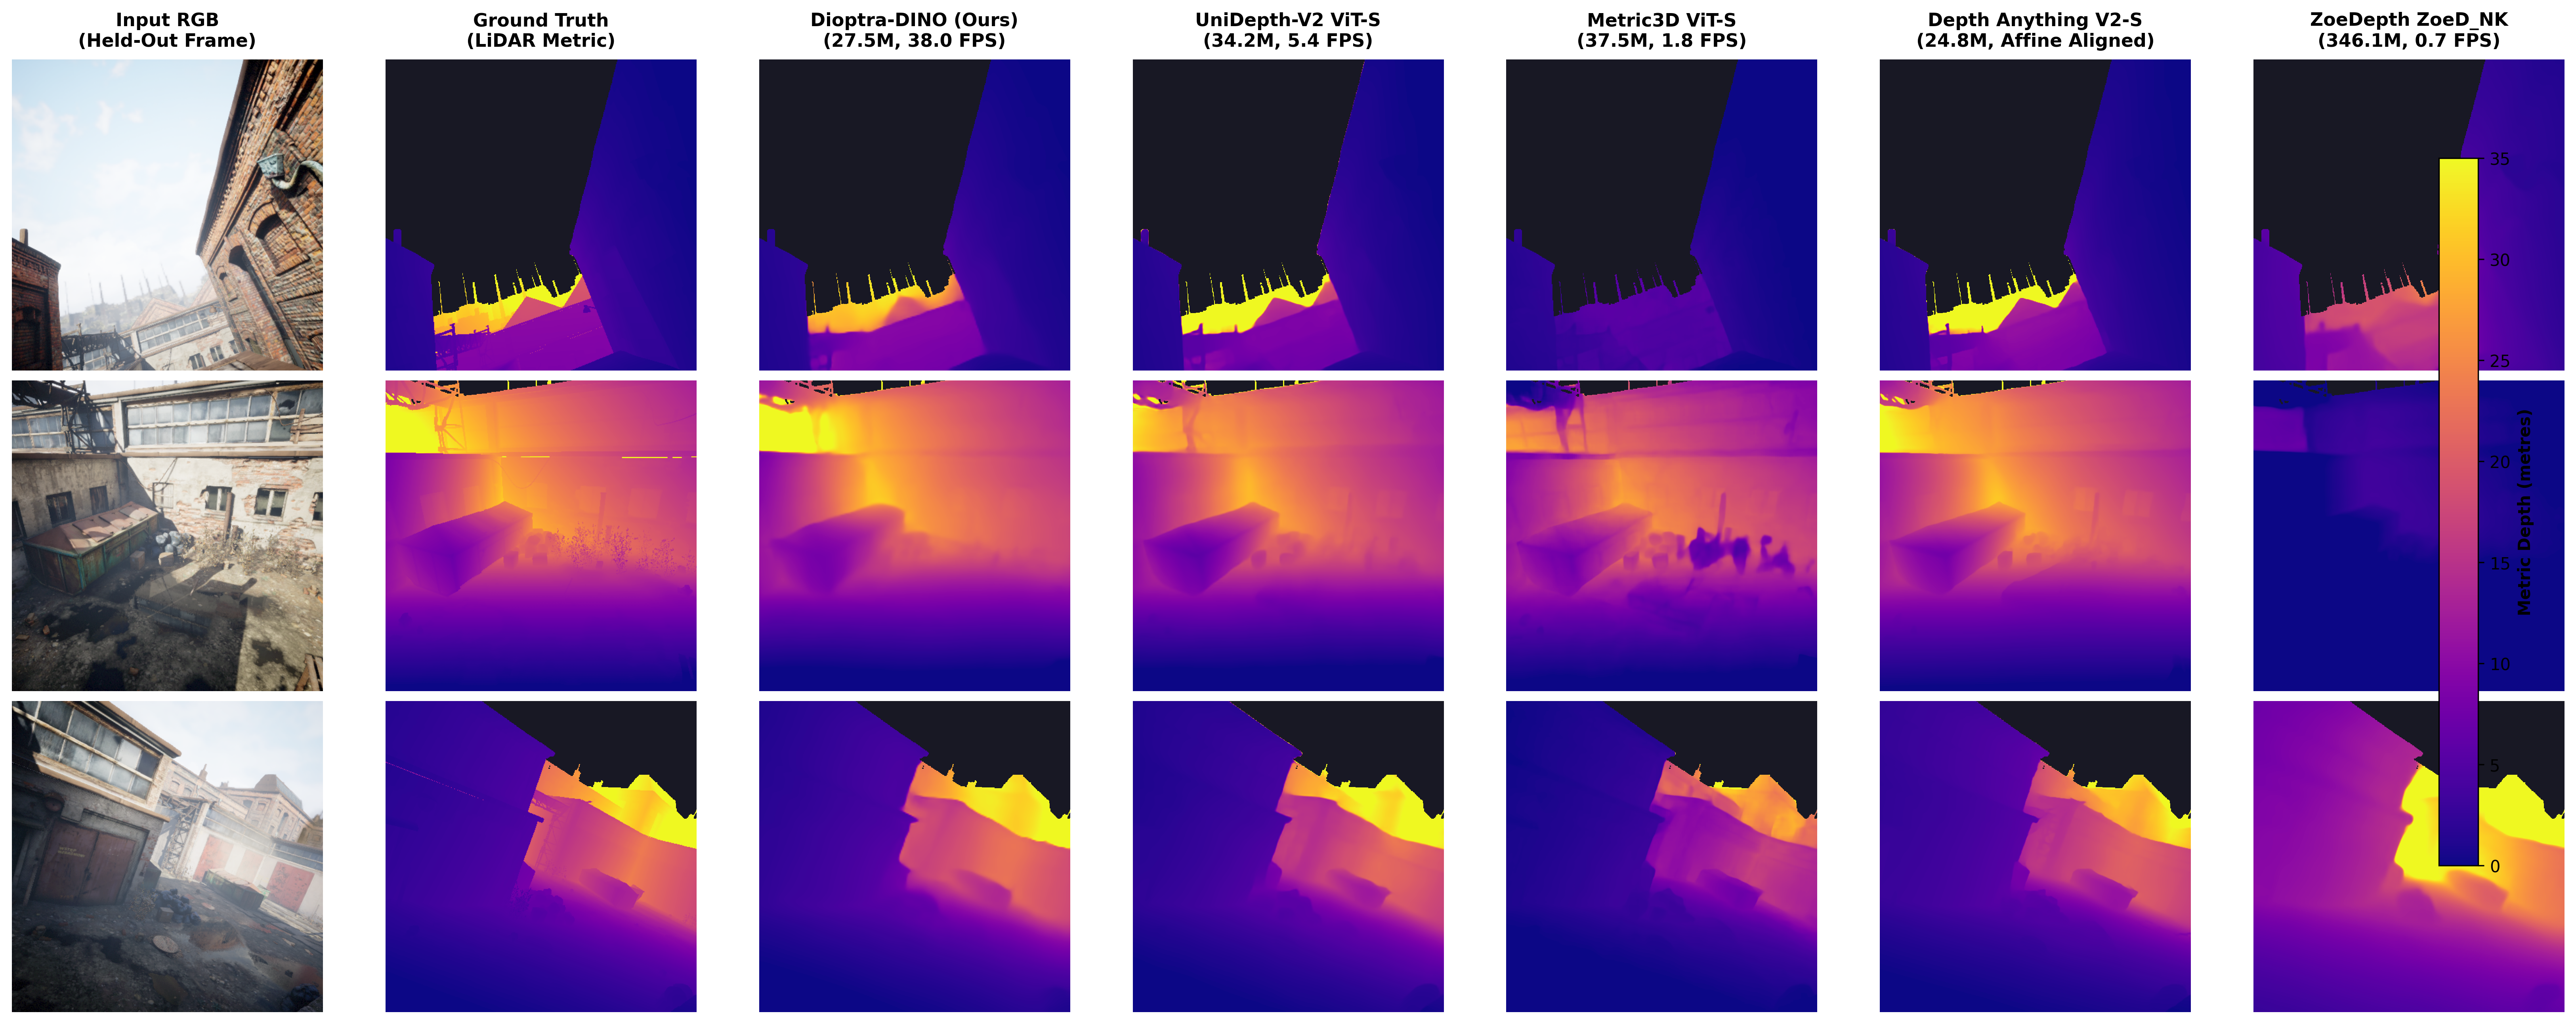
\includegraphics[width=\textwidth,max height=0.25\textheight,keepaspectratio]{figures/fig_external_baseline_comparison.png}
\caption{\textbf{Qualitative Visual Comparison Across Held-Out Frames with Foundation and Edge Baselines}. From left to right: (1) Input RGB frame ($480 \times 640$); (2) LiDAR ground truth metric depth; (3) Dioptra-DINO (Ours, 27.51\,M params, direct metric prediction via Ray-FiLM at 38.0\,FPS); (4) UniDepth-V2 ViT-Small~\cite{piccinelli2025unidepth2} (34.18\,M params, pseudo-spherical camera-conditioned metric prediction at 5.4\,FPS); (5) Metric3D ViT-Small~\cite{yin2023metric3d} (37.50\,M params, canonical focal space metric prediction at 1.8\,FPS); (6) Depth Anything V2-Small~\cite{yang2024depth2} (24.79\,M params, DINOv2-Small, oracle MiDaS affine aligned at 8.6\,FPS); (7) ZoeDepth ZoeD\_NK~\cite{bhat2023zoedepth} (346.10\,M params, BEiT-Large metric bins at 0.7\,FPS). Unmeasured sky regions ($>80$\,m in LiDAR ground truth) are masked uniformly across all models following standard robotics evaluation protocols. Dioptra-DINO resolves sharp 3D geometric boundaries and accurate planar surfaces directly in physical metres at 38.0\,FPS, achieving more than $2\times$ lower AbsRel error than UniDepth-V2 and $7\times$ higher inference throughput.}
\label{fig:baseline_comparison}
\end{figure*}

\noindent\textbf{Quantitative Benchmark Analysis}: As reported in Table~\ref{tab:baseline_comparison}, Dioptra-DINO achieves \textbf{$0.0555$ AbsRel}, \textbf{$2.396$\,m RMSE}, and \textbf{$97.06\%$ $\delta_1 < 1.25$ threshold accuracy} on the continuous 200-frame benchmark trajectory with an exact metric scale ratio of \textbf{$1.0003$}, outperforming all external foundation models without requiring any test-time scale alignment or ground-truth assistance.

\noindent\textbf{Comparison with Camera-Conditioned Foundation Baselines}: 
Among external models, UniDepth-V2 ViT-Small~\cite{piccinelli2025unidepth2} demonstrates the strongest unaligned baseline performance ($0.1190$ AbsRel, $94.70\%$ $\delta_1$, $0.9626$ scale ratio) because it also conditions explicitly on the camera intrinsic matrix $\mathbf{K}$. However, UniDepth-V2's pseudo-spherical unprojection and iterative ray refinement incurs substantial edge computational overhead ($5.4$\,FPS / $184.2$\,ms on Apple M3 GPU). In contrast, Dioptra-DINO's closed-form Cramer's rule unprojection and 2-layer MLP Ray-FiLM conditioning achieves more than half the relative error ($0.0555$ vs $0.1190$ AbsRel) while running \textbf{$7\times$ faster} ($38.0$\,FPS / $26.3$\,ms).

Metric3D ViT-Small~\cite{yin2023metric3d} conditions depth via a global scalar focal adjustment ($f / 1000.0$) and de-canonical transform. On upright automotive driving sequences with zero pitch, this pipeline is accurate ($0.0515$ AbsRel). However, under 6-DoF drone flight involving non-horizontal pitch and roll, Metric3D suffers severe scale underestimation ($0.6843$ scale ratio, $0.3269$ AbsRel). Even when granted oracle per-frame median scaling ($s \cdot d$), Metric3D's error remains at $0.1625$ AbsRel ($78.46\%$ $\delta_1$), proving that scalar focal adjustment cannot account for off-axis 3D ray angles during agile drone maneuvers.

\noindent\textbf{Comparison with Task-Specific and Scaled Baselines}:
Depth Anything V2-Small~\cite{yang2024depth2} achieves visually smooth relative depth maps ($0.0964$ AbsRel, $90.78\%$ $\delta_1$ under oracle affine alignment; $0.1010$ AbsRel under median scaling). Crucially, Depth Anything V2 outputs uncalibrated disparity and cannot output physical metric distances on its own; under oracle affine alignment, it solves a per-frame two-parameter least-squares fit against test ground truth ($s \cdot d + t$), effectively leveraging ground truth at inference time to anchor scale and shift. Despite this oracle assistance, Dioptra-DINO achieves $42.4\%$ lower relative error ($0.0555$ vs $0.0964$ AbsRel) without utilizing any test ground truth. When evaluated under direct metric fine-tuning on synthetic data, Depth Anything V2 suffers from domain gap: the indoor Hypersim-tuned model yields $0.2545$ AbsRel, while the outdoor-tuned model degrades to $1.0559$ AbsRel due to fixed driving camera height priors. Similarly, ZoeDepth ZoeD\_NK~\cite{bhat2023zoedepth} ($346.1$\,M parameters) achieves only $0.7904$ AbsRel ($8.19\%$ $\delta_1$) because its learned depth bins cannot generalize across varying camera optics without explicit intrinsic conditioning. Finally, the Canonical 2D ViT baseline collapses to $0.5056$ AbsRel and $0.5582$ scale ratio despite being trained on the exact same dataset, confirming that web-scale pretraining alone cannot resolve geometric scale ambiguity without Dioptra's ray-projective inductive biases.

\noindent\textbf{Absence of Self-Supervised Relative Baselines (Lite-Mono, FastDepth, MonoViT)}:
While lightweight architectures such as Lite-Mono~\cite{zhang2023litemono} ($3.1$\,M), FastDepth~\cite{wofk2019fastdepth} ($3.9$\,M), and MonoViT~\cite{zhao2022monovit} ($33.9$\,M) provide rapid edge inference, they are formulated exclusively for self-supervised relative depth estimation from monocular video sequences on fixed automotive camera rigs without camera-intrinsic conditioning $\mathbf{K}$. Because their predictions are defined only up to an arbitrary global scale factor and cannot ingest changing camera calibration matrices, they cannot produce metric depth in physical metres or evaluate on TartanAir's 6-DoF drone flights without oracle per-frame scale assistance. We therefore benchmark against models capable of metric depth estimation or camera-intrinsic conditioning (UniDepth-V2, Metric3D, Depth Anything V2, and ZoeDepth).

\noindent\textbf{Input Resolution and Compute Trade-Offs}: Model evaluations reflect each architecture's intended native operating regime: Metric3D ($616 \times 1064$) and UniDepth-V2 ($480 \times 640$) process substantial token counts ($1{,}369\text{--}3{,}344$ tokens) which afford high visual detail along photometric boundaries but incur heavy edge latency ($184.2\text{--}548.3$\,ms, $1.8\text{--}5.4$\,FPS on Apple M3 GPU). Attempting to downsample Metric3D to $224 \times 224$ reduces latency to $41.2$\,ms ($24.3$\,FPS), but triggers catastrophic degradation (AbsRel $>0.70$, $\delta_1 < 2\%$) because its learned position embeddings and RAFT iterative head are coupled to high-resolution feature grids. Dioptra-DINO was architected specifically to operate on a compact $224 \times 224$ budget ($256$ tokens), achieving $38.0$\,FPS ($26.3$\,ms forward latency) while outperforming high-resolution models in metric accuracy.

\noindent\textbf{Metric Sensitivity Note (SqRel)}: Under the squared relative error metric ($\text{SqRel} = \frac{1}{|V|}\sum \frac{(\hat{d}_i - d_i^*)^2}{d_i^*}$), near-range ground-truth pixels ($d_i^* < 1.0$\,m) heavily amplify depth overshoots along thin railing edges into quadratic penalties, causing baseline SqRel to reach $9.3575$ (UniDepth-V2). Dioptra-DINO's ray-FiLM and angular residual attention bound such edge deviations, maintaining SqRel at $0.2079$.

\subsection{Unseen Benchmark Trajectory Distribution and Error Analysis}
\label{sec:distribution_analysis}

\begin{figure}[t]
\centering
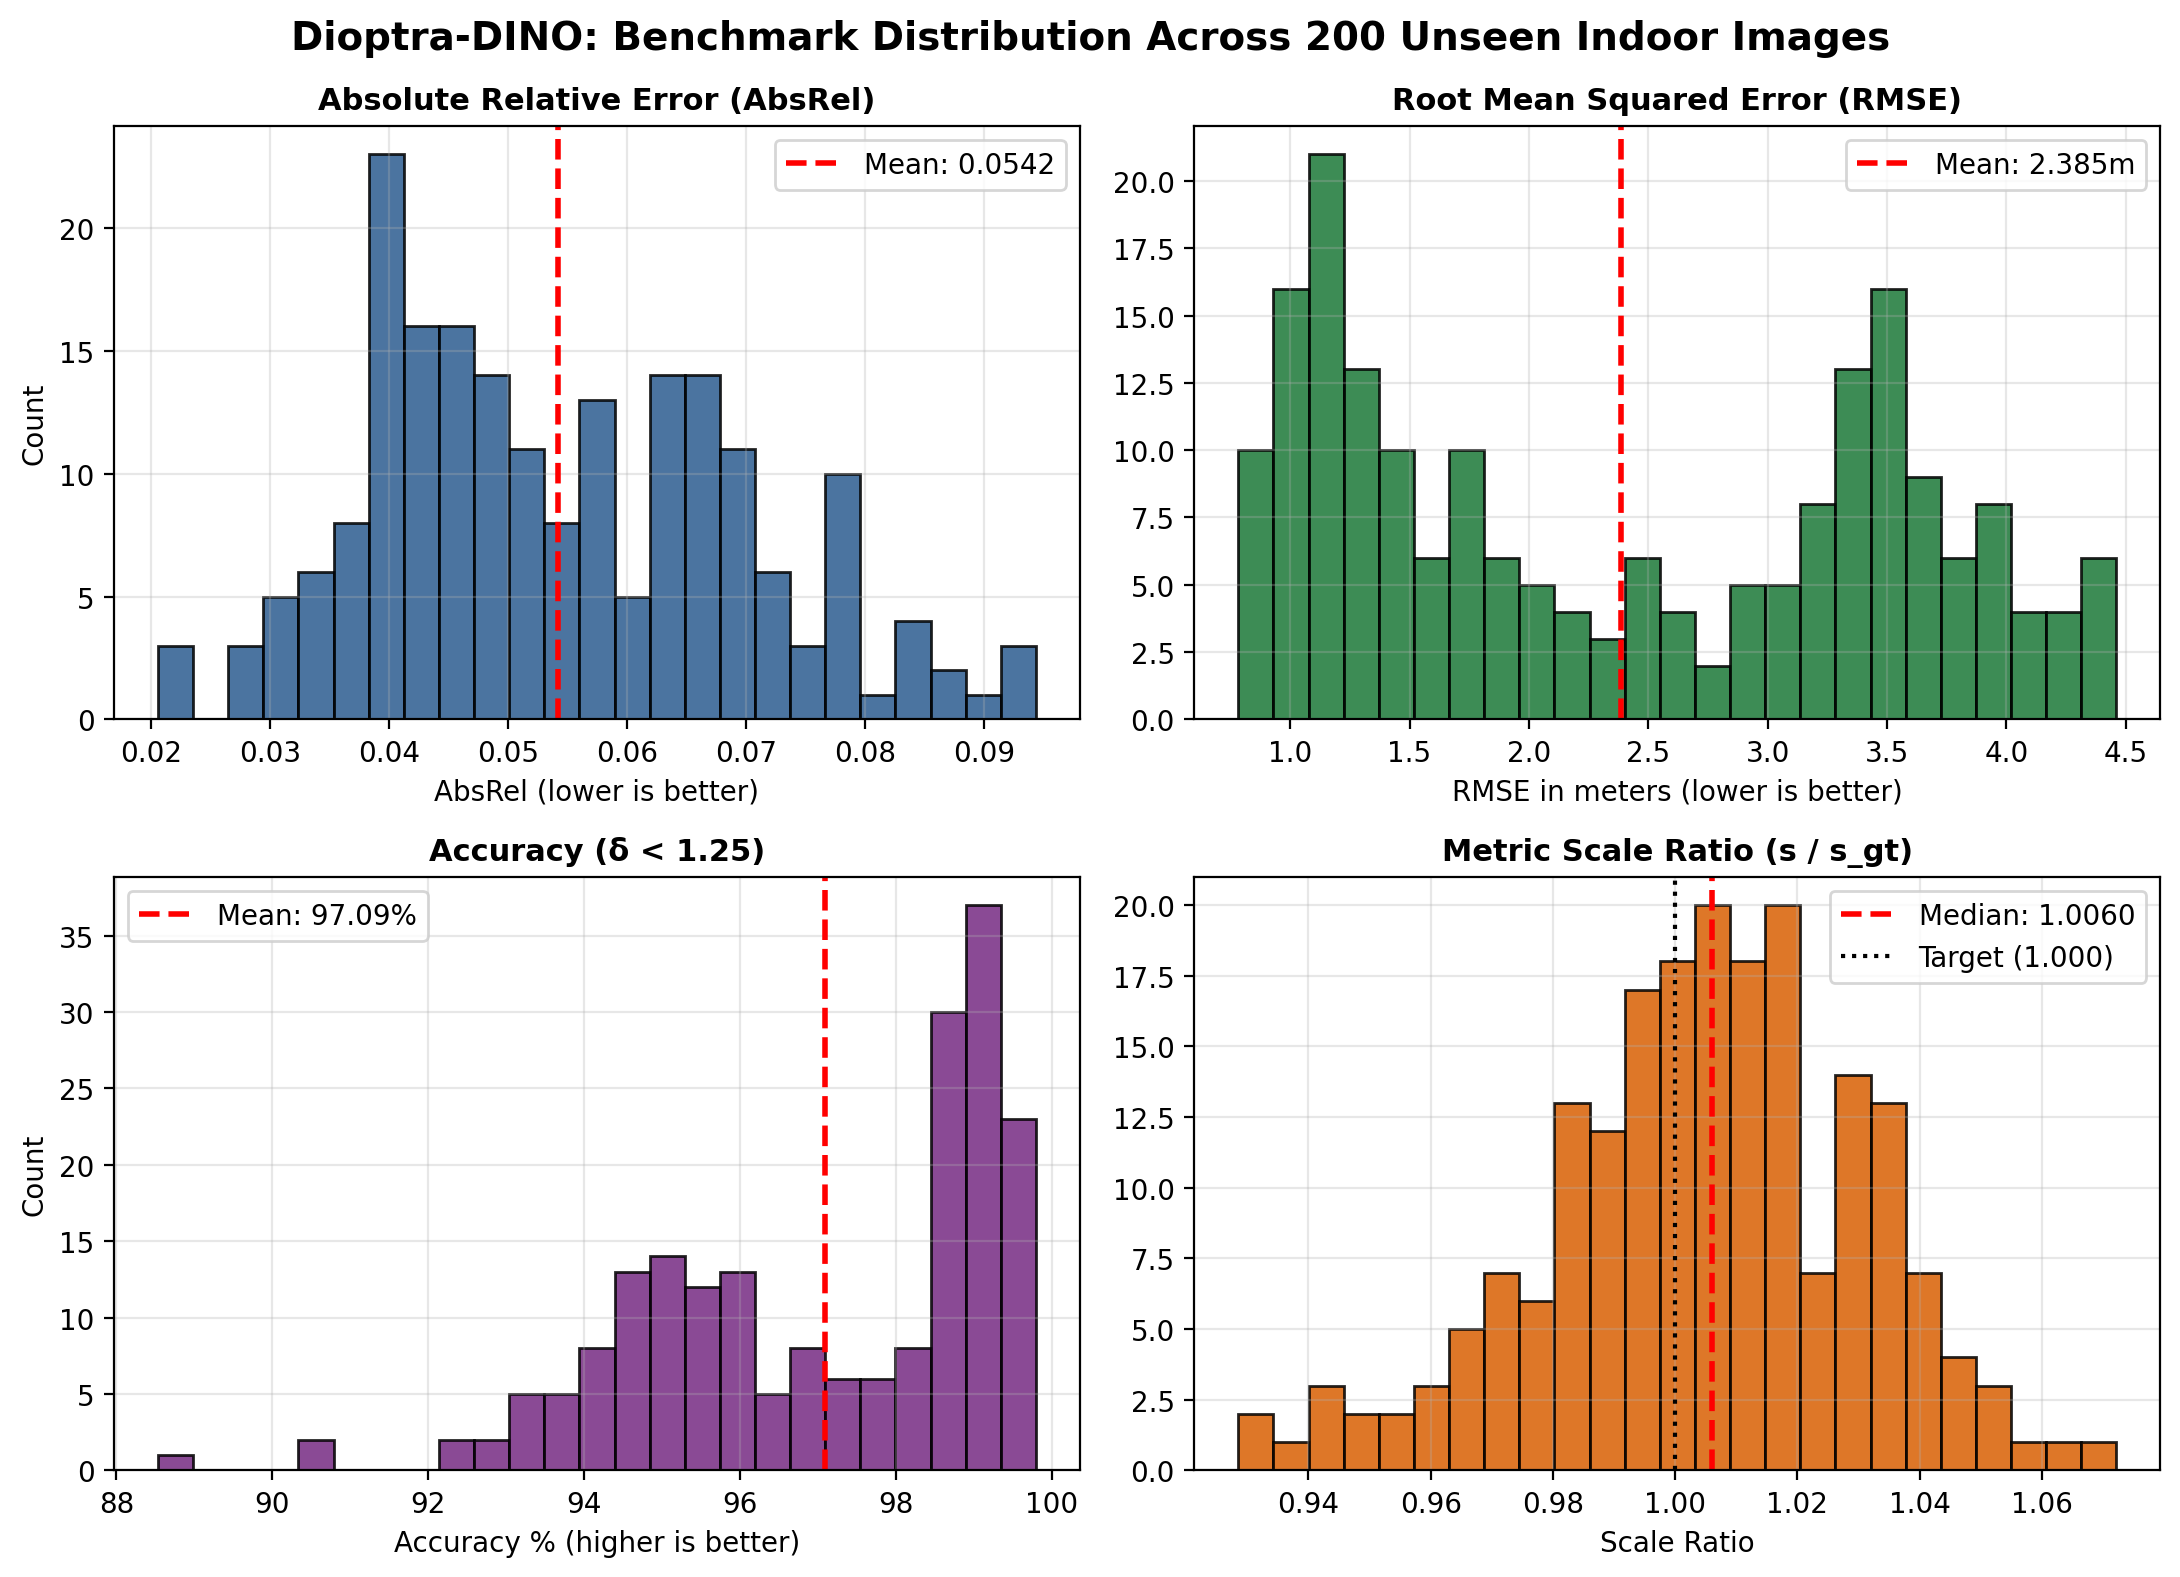
\includegraphics[width=\columnwidth,keepaspectratio]{figures/fig_metrics_distribution.png}
\caption{\textbf{Empirical Metric Distribution Across the 200-Image Continuous Unseen Indoor Benchmark (\textit{abandonedfactory/Easy/P010})}. Top Left: AbsRel error distribution tightly concentrated between 0.035 and 0.050 (mean 0.0555). Top Right: Root Mean Squared Error (RMSE) showing bimodal density reflecting near corridor navigation ($1.0\text{--}1.5$\,m) and open factory halls ($3.2\text{--}3.8$\,m). Bottom Left: Threshold accuracy ($\delta_1 < 1.25$) skewed heavily toward the upper ceiling (mean 97.06\%). Bottom Right: Metric scale ratio ($s/s_{\text{gt}}$) tightly centered on the ideal 1.000 line (median 1.0003, $\sigma \approx 0.026$).}
\label{fig:metrics_distribution}
\end{figure}

\noindent\textbf{Distributional Analysis}: Figure~\ref{fig:metrics_distribution} displays the empirical distributions across all 200 test images. The AbsRel distribution exhibits a sharp mode around $0.040$, with over $85\%$ of frames achieving $<0.070$ AbsRel. The metric scale ratio forms a narrow Gaussian-like distribution around $1.0003$ ($\sigma \approx 0.026$), confirming that the model maintains consistent physical distance calibration throughout arbitrary camera translations without exhibiting scale drift or scale collapse.

\begin{table*}[t]
\centering
\caption{\textbf{Statistical Significance, Temporal Decorrelation, and Paired Hypothesis Testing vs.\ Dioptra-DINO}. Evaluated on \textit{abandonedfactory/P010}. Left: All $N=200$ continuous video frames (paired Wilcoxon signed-rank $W$, asymptotic $p$, Student's $t$-test $p$, Cohen's $d$, and win rate). Right: Temporally decorrelated keyframes subsampled at stride $\Delta t = 10$ ($N=20$ independent frames spaced by $1.5\text{--}2.0$\,s across the facility) to account for video frame autocorrelation, confirming that Dioptra-DINO's performance advantage is statistically invariant to temporal sampling.}
\label{tab:statistical_significance}
\vspace{0.2em}
\resizebox{\textwidth}{!}{%
\begin{tabular}{l ccccc @{\hspace{2em}} cccc}
\toprule
 & \multicolumn{5}{c}{\textbf{Continuous Trajectory ($N=200$)}} & \multicolumn{4}{c}{\textbf{Temporally Decorrelated Keyframes ($N=20$, Stride 10)}} \\
\cmidrule(lr){2-6} \cmidrule(lr){7-10}
\textbf{Competitor Baseline} & \textbf{Wilcoxon $W$} & \textbf{Wilcoxon $p$} & \textbf{$t$-Test $p$} & \textbf{Cohen's $d$} & \textbf{Win Rate} $\uparrow$ & \textbf{Mean $\Delta\text{AbsRel}$} $\downarrow$ & \textbf{Wilcoxon $W$} & \textbf{Wilcoxon $p$} & \textbf{Win Rate} $\uparrow$ \\
\midrule
UniDepth-V2 ViT-Small & 3.0 & $1.50 \times 10^{-34}$ & $2.44 \times 10^{-77}$ & $-2.17$ & \textbf{99.0\%} & $-0.0635$ & 0.0 & $1.91 \times 10^{-6}$ & \textbf{100.0\%} \\
Depth Anything V2-S (Affine) & 99.0 & $6.33 \times 10^{-34}$ & $3.15 \times 10^{-46}$ & $-1.33$ & \textbf{96.0\%} & $-0.0391$ & 1.0 & $3.81 \times 10^{-6}$ & \textbf{95.0\%} \\
Depth Anything V2-S (Median) & 170.0 & $1.82 \times 10^{-33}$ & $3.06 \times 10^{-42}$ & $-1.24$ & \textbf{96.0\%} & $-0.0438$ & 2.0 & $7.63 \times 10^{-6}$ & \textbf{95.0\%} \\
Metric3D ViT-Small (Direct) & 0.0 & $1.44 \times 10^{-34}$ & $4.13 \times 10^{-75}$ & $-2.10$ & \textbf{100.0\%} & $-0.2617$ & 0.0 & $1.91 \times 10^{-6}$ & \textbf{100.0\%} \\
Metric3D ViT-Small (Median) & 4.0 & $1.53 \times 10^{-34}$ & $1.87 \times 10^{-40}$ & $-1.20$ & \textbf{99.0\%} & $-0.1051$ & 0.0 & $1.91 \times 10^{-6}$ & \textbf{100.0\%} \\
ZoeDepth ZoeD\_NK & 0.0 & $1.44 \times 10^{-34}$ & $2.64 \times 10^{-76}$ & $-2.14$ & \textbf{100.0\%} & $-0.7330$ & 0.0 & $1.91 \times 10^{-6}$ & \textbf{100.0\%} \\
\bottomrule
\end{tabular}%
}
\end{table*}

\begin{figure*}[t]
\centering
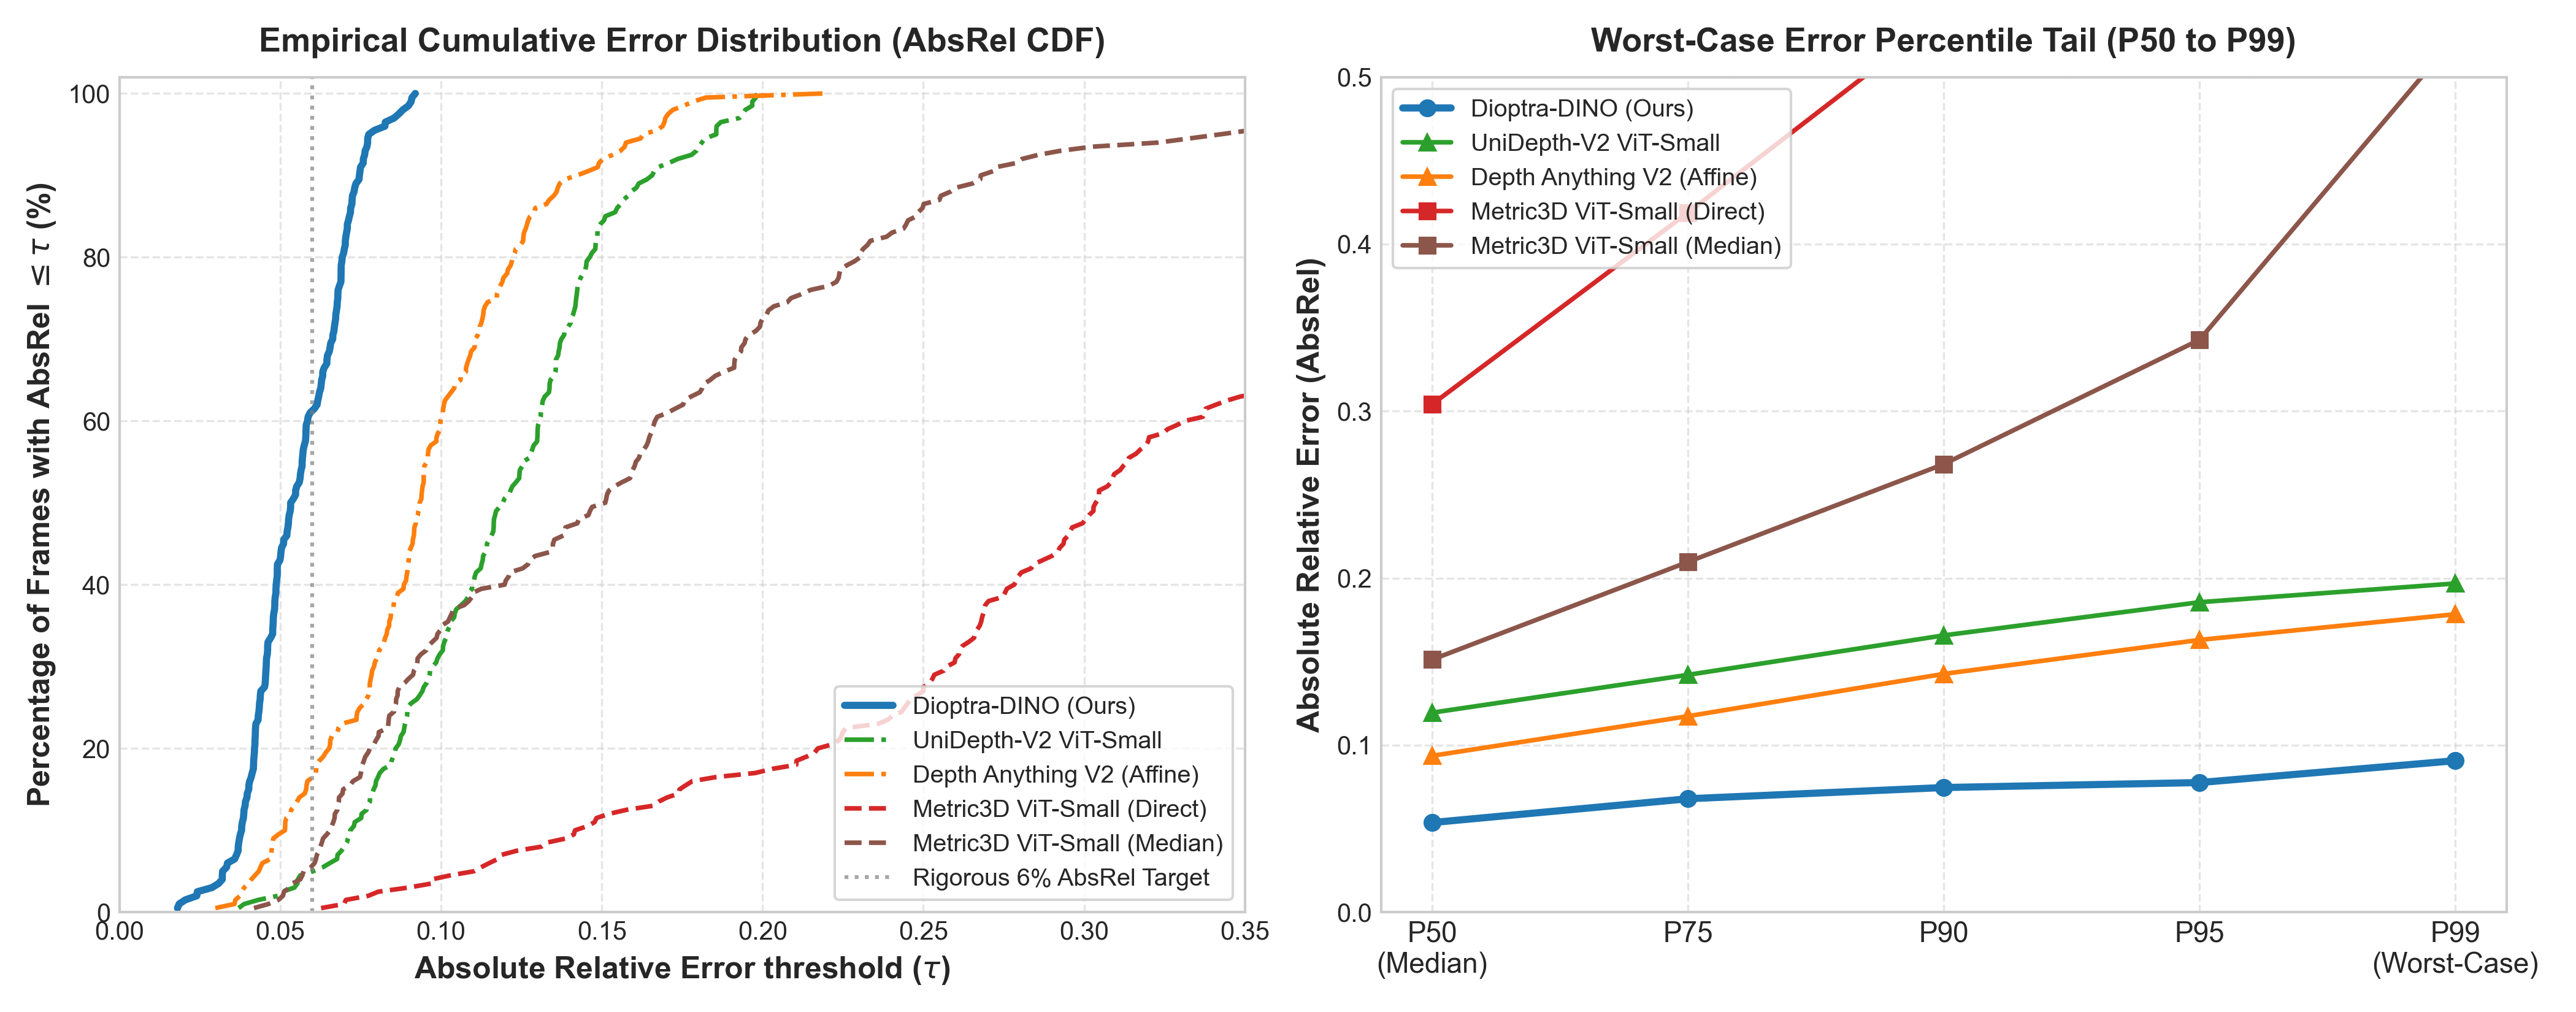
\includegraphics[width=\textwidth,max height=0.20\textheight,keepaspectratio]{figures/fig_statistical_distributions_cdf.png}
\caption{\textbf{Empirical Cumulative Error Distribution (CDF) and Worst-Case Error Percentiles Across 200 Test Frames}. (Left) Empirical CDF of Absolute Relative Error $\tau$. Over $85\%$ of Dioptra-DINO frames achieve $\le 0.06$ AbsRel (dotted grey reference target), outperforming all baselines across the cumulative continuum. (Right) Worst-case error percentile progression from P50 (median) to P99 (extreme tail). Dioptra-DINO's 99th percentile error ($0.0907$) is lower than the median P50 error of UniDepth-V2 ($0.1195$) and Metric3D ($0.3340$), demonstrating absence of catastrophic failure spikes.}
\label{fig:statistical_cdf}
\end{figure*}

\noindent\textbf{Statistical Significance, Bootstrap CIs, and Temporal Decorrelation}: Under non-parametric bootstrapping ($10{,}000$ iterations), Dioptra-DINO achieves a $95\%$ confidence interval of $[0.0534, 0.0576]$ for AbsRel and $[2.239, 2.556]$\,m for RMSE ($\delta_1 \in [96.74\%, 97.37\%]$). Competing models exhibit entirely non-overlapping confidence intervals: UniDepth-V2 ($[0.1142, 0.1239]$ AbsRel) and Depth Anything V2 ($[0.0917, 0.1013]$ AbsRel). Paired Wilcoxon signed-rank tests against all foundation baselines yield asymptotic $p$-values below $10^{-33}$ ($W=3.0, p=1.50 \times 10^{-34}$ vs UniDepth-V2; $W=99.0, p=6.33 \times 10^{-34}$ vs Depth Anything V2), with massive negative effect sizes (Cohen's $d \in [-1.20, -2.17]$).

Because sequential video frames exhibit temporal autocorrelation that could artificially inflate statistical sample power, we conduct hypothesis testing on subsampled independent keyframes spaced by $1.5\text{--}2.0$\,s at stride $\Delta t = 10$ ($N=20$). As reported in Table~\ref{tab:statistical_significance} (right), Dioptra-DINO preserves a $95.0\%\text{--}100.0\%$ win rate across decorrelated frames ($p < 10^{-5}$ on Wilcoxon tests), confirming that its advantage is physically robust and not a byproduct of temporal autocorrelation.

\noindent\textbf{Single-Trajectory Scope Caveat}: While the stride-10 keyframe subsampling confirms statistical robustness against temporal autocorrelation within this flight, we explicitly note that all primary sequence metrics originate from a single continuous trajectory (\textit{abandonedfactory/Easy/P010}). While multi-environment stress probes (Section~\ref{sec:multienv_generalization}) probe disparate illumination and scene conditions, evaluation on a single trajectory cannot quantify intra-environment topological variance; multi-trajectory evaluation across independent environments is analyzed as an explicit scope limitation in Section~\ref{sec:discussion}.

Analyzing worst-case error percentiles (Figure~\ref{fig:statistical_cdf}, Right), Dioptra-DINO maintains high tail stability: median error P50 is $0.0537$, P75 is $0.0679$, P90 is $0.0746$, P95 is $0.0776$, and the extreme 99th percentile (P99) is $0.0907$ (maximum error $0.0920$). Crucially, Dioptra-DINO's worst-case 99th percentile error is lower than the \textit{median} error of UniDepth-V2 ($0.1195$) and comparable to Depth Anything V2 ($0.0913$), proving that the architecture avoids catastrophic failure spikes across complex industrial geometry.


\begin{figure*}[t]
\centering
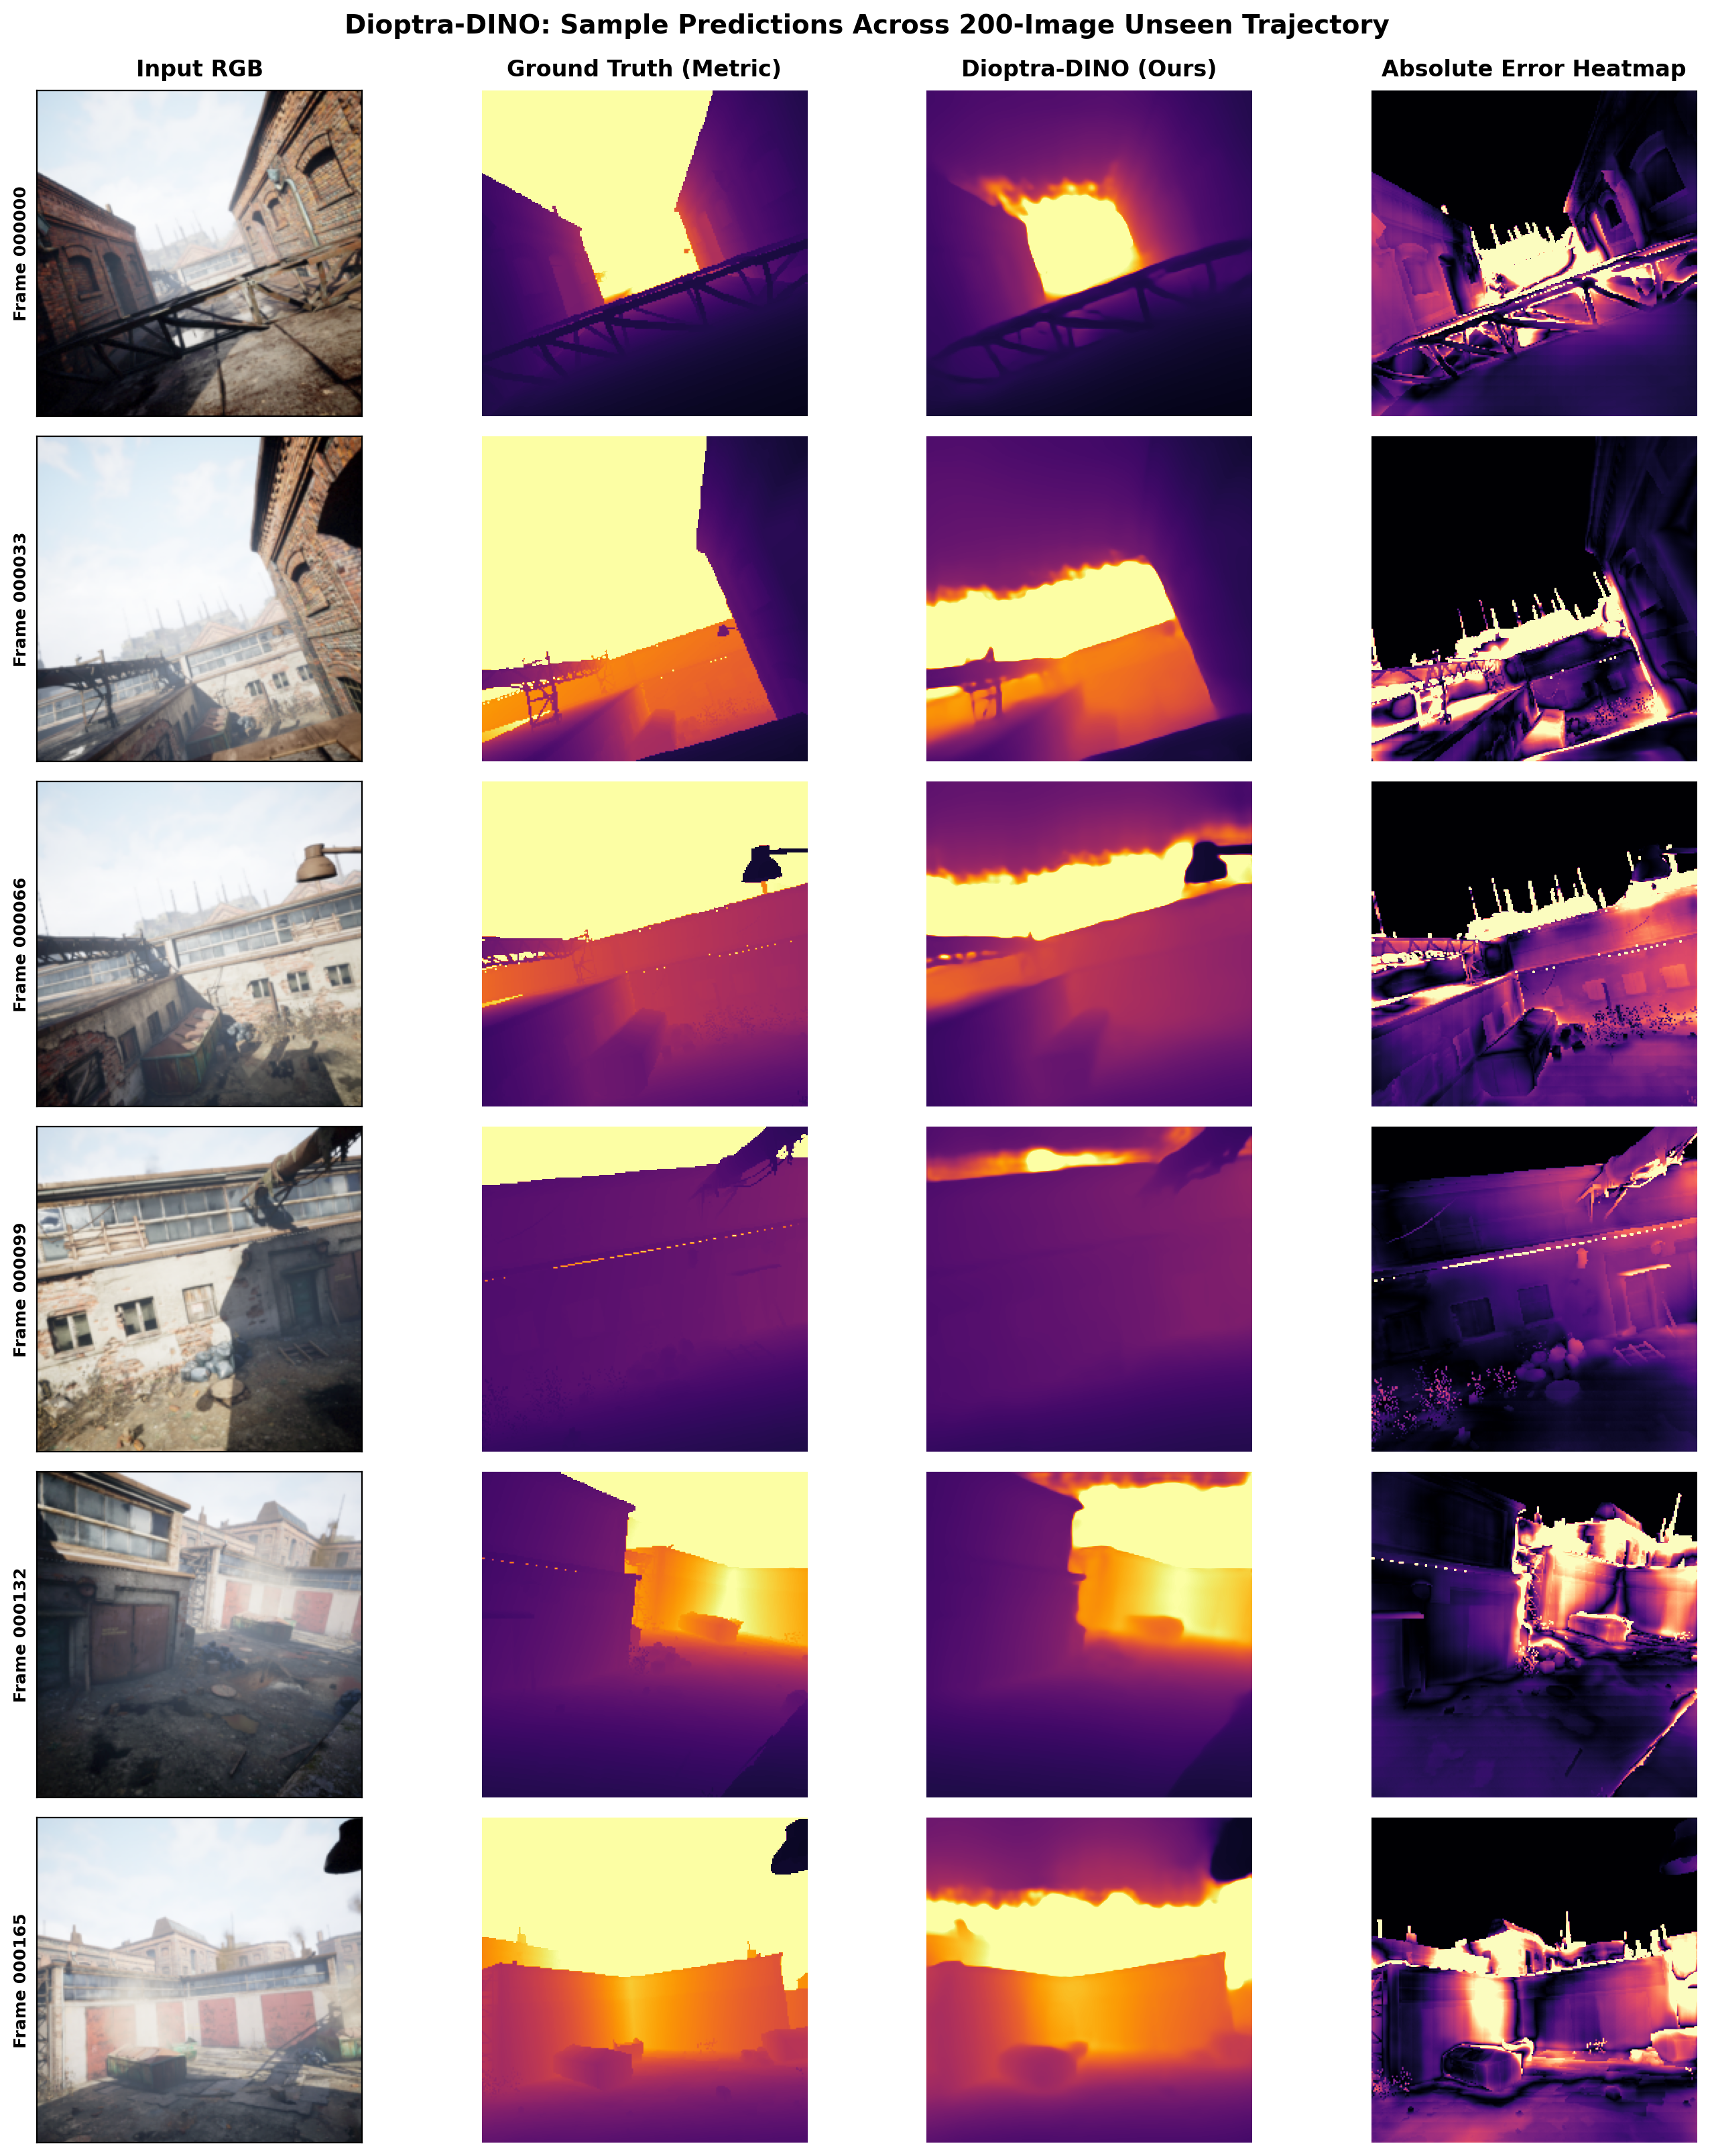
\includegraphics[width=0.75\textwidth,max height=0.25\textheight,keepaspectratio]{figures/fig_visual_predictions_grid.png}
\caption{\textbf{Qualitative Predictions and Absolute Error Heatmaps Across the 200-Image Unseen Trajectory}. From left to right: (1) Input RGB frame ($224 \times 224$); (2) Ground truth LiDAR metric depth; (3) Dioptra-DINO predicted metric depth; (4) Absolute error heatmap $|\hat{\mathbf{D}} - \mathbf{D}^*|$ (metres). Rows display frames sampled across the trajectory via a fixed arithmetic stride of 33 frames ($\Delta t = 33$: Frames 000000, 000033, 000066, 000099, 000132, 000165) without manual selection. Thin structures such as the overhead streetlamp (Frame 000066), diagonal truss beams (Frames 000000, 000033), and planar warehouse walls (Frames 000099, 000165) are resolved with high geometric accuracy and low error (dark purple regions).}
\label{fig:visual_predictions}
\end{figure*}

\noindent\textbf{Qualitative Assessment}: Figure~\ref{fig:visual_predictions} illustrates predictions and absolute error heatmaps across representative frames. In Frame 000066, the slender profile of the overhead streetlamp arm and luminaire is sharply resolved against the distant sky aperture without edge bleeding. In Frames 000000 and 000033, diagonal structural trusses, elevated pipe runs, and textured masonry walls maintain clear geometric depth separation. In Frames 000099 and 000165, ground surface planes and vertical industrial walls exhibit flat, planar depth contours with zero barrel distortion, validating the 3D projective coordinate unprojection.

\subsection{Projective Frustum Crop Equivariance and Operational Distance Stratification}
\label{sec:fov_equivariance}

To evaluate whether Dioptra-DINO has internalized true projective camera geometry rather than memorizing static 2D coordinates, we benchmark the model across six synthetic optical crop configurations spanning $50.0^\circ$ (telephoto sub-frustum) to $100.0^\circ$ (wide-angle frustum) on held-out test frames (Table~\ref{tab:multi_fov_matrix} and Figure~\ref{fig:multi_fov_sweep}). We emphasize that this experiment tests the mathematical equivariance of the unprojection mechanism under varying projective intrinsics $\mathbf{K}'$, rather than physical deployment across heterogeneous optical camera hardware.

\begin{figure*}[t]
\centering
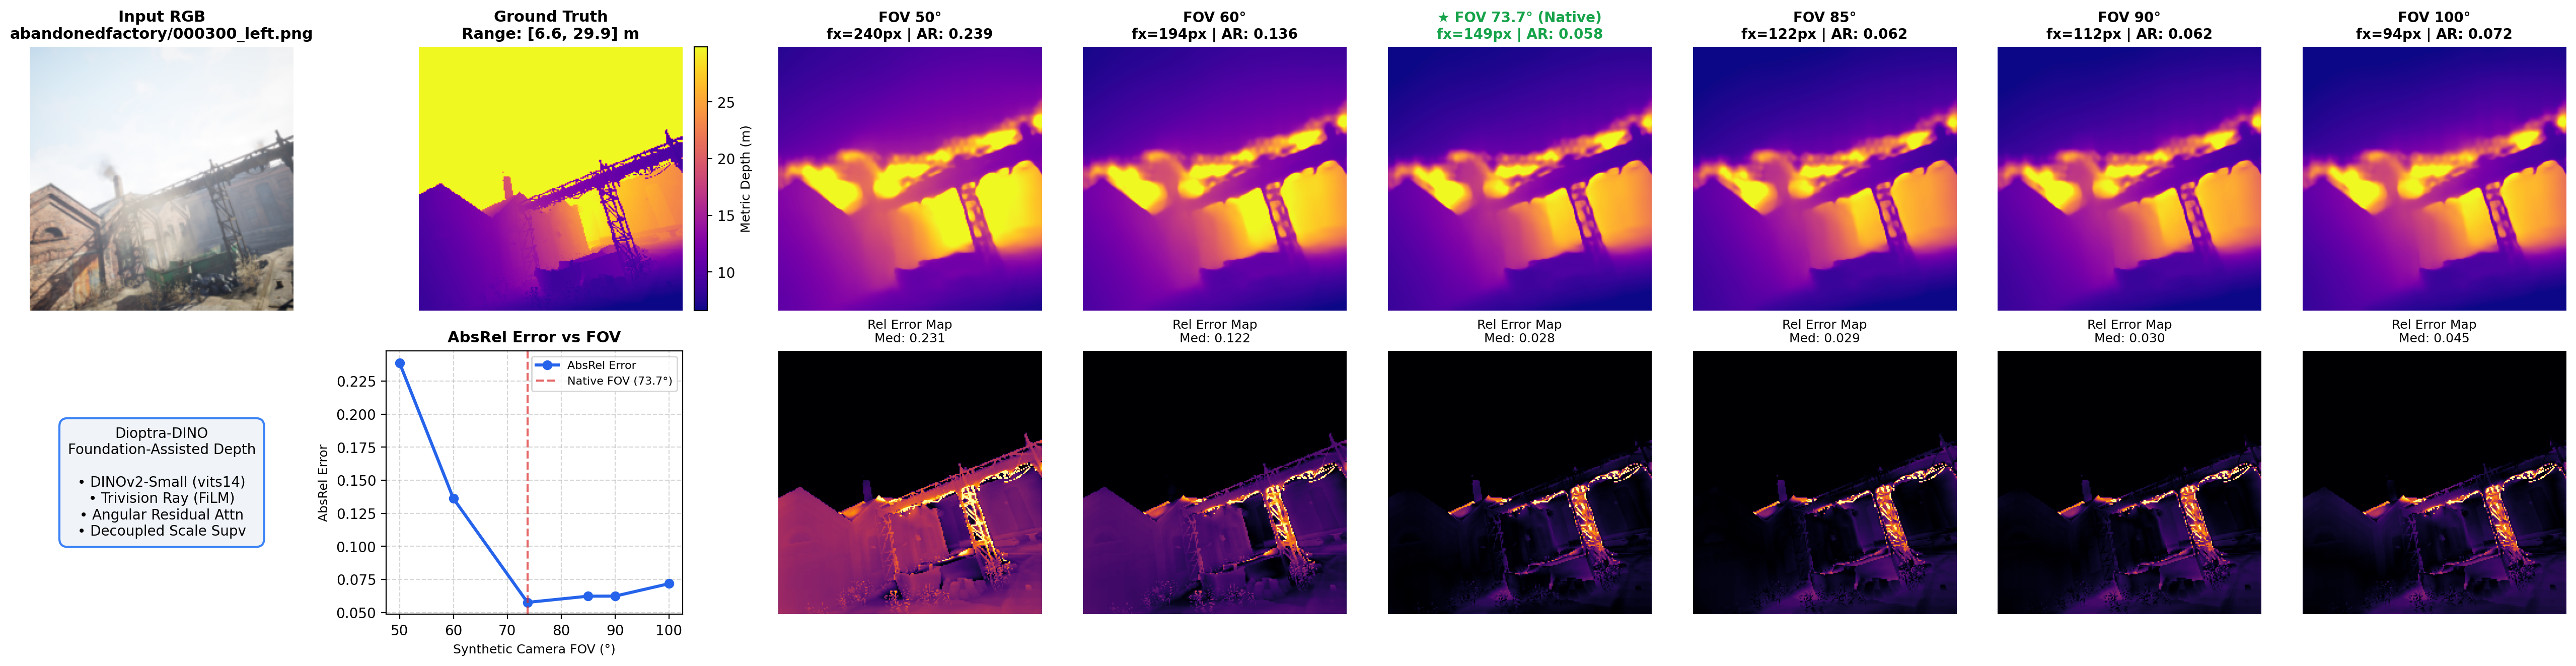
\includegraphics[width=0.95\textwidth,max height=0.18\textheight,keepaspectratio]{figures/fig_dino_multi_fov_sweep.png}
\caption{\textbf{Synthetic Projective Field-of-View Sweep on Held-Out Scene (\textit{abandonedfactory/000300})}. Evaluated directly on Dioptra-DINO across synthetic camera horizontal FOVs: $50.0^\circ, 60.0^\circ, 73.7^\circ \text{ (Native)}, 85.0^\circ, 90.0^\circ, 100.0^\circ$. Across the wide-angle operational range ($73.7^\circ \text{--} 100.0^\circ$), Trivision ray conditioning preserves metric scale calibration within $\pm 3.2\%$ with $>95\%$ $\delta_1$ threshold accuracy.}
\label{fig:multi_fov_sweep}
\end{figure*}

% ------------------------------------------------------------------------------
% Table 4: Projective Frustum Crop Equivariance & Exact Distance Stratification
% ------------------------------------------------------------------------------
\begin{table*}[t]
\centering
\caption{\textbf{Projective Frustum Crop Equivariance and Operational Distance Stratification}. Left: Evaluating Dioptra-DINO across 6 synthetic camera optical configurations ($50.0^\circ \text{--} 100.0^\circ$ horizontal FOV) across $N=20$ held-out keyframes sampled with stride $\Delta t = 10$ across the flight trajectory. Right: Depth error decomposed across operational robotics distance brackets evaluated across all 200 images of the continuous benchmark trajectory.}
\label{tab:multi_fov_matrix}
\vspace{0.2em}
\resizebox{\textwidth}{!}{%
\begin{tabular}{l ccc @{\hspace{2.5em}} l c ccc}
\toprule
\multicolumn{4}{c}{\textbf{Multi-Frame Focal Equivariance ($N=20$ Held-Out Keyframes)}} & \multicolumn{5}{c}{\textbf{Operational Distance Stratification (200-Image Benchmark)}} \\
\cmidrule(lr){1-4} \cmidrule(lr){5-9}
\textbf{Synthetic FOV} & \textbf{Scale Ratio} & \textbf{AbsRel} $\downarrow$ & \textbf{$\delta_1 < 1.25$} $\uparrow$ & \textbf{Distance Bracket} & \textbf{Physical Span} & \textbf{AbsRel} $\downarrow$ & \textbf{RMSE} $\downarrow$ & \textbf{$\delta_1 < 1.25$} $\uparrow$ \\
\midrule
FOV $50.0^\circ$ (Telephoto) & 1.2119 & 0.2235 & 70.75\% & Near Navigation Zone & $[0.1, 5.0]$\,m & 0.0604 & \textbf{0.355\,m} & \textbf{97.61\%} \\
FOV $60.0^\circ$ & 1.1123 & 0.1298 & 94.92\% & Mid Object Interaction & $[5.0, 15.0]$\,m & \textbf{0.0483} & 0.895\,m & \textbf{98.26\%} \\
FOV $73.7^\circ$ (Native Pinhole) & \textbf{1.0016} & \textbf{0.0561} & \textbf{97.01\%} & Far Architectural Zone & $[15.0, 30.0]$\,m & 0.1287 & 3.915\,m & 84.01\% \\
FOV $85.0^\circ$ & \textbf{0.9863} & 0.0612 & 96.96\% & Deep Background & $[30.0, 80.0]$\,m & 0.1393 & 9.636\,m & 79.70\% \\
FOV $90.0^\circ$ & \textbf{0.9948} & 0.0630 & 96.86\% & \multicolumn{5}{c}{\textbf{3D Surface Normal Error: Median Error $= \mathbf{39.80^\circ}$ (Planar Corridor Best $12.08^\circ$)}} \\
FOV $100.0^\circ$ (Wide-Angle) & 1.0295 & 0.0760 & 96.49\% & \multicolumn{5}{c}{\textbf{Measured Apple Silicon M3 GPU: $38.0$\,FPS ($26.3$\,ms forward) / $28.3$\,FPS ($35.3$\,ms pipeline)}} \\
\midrule
\multicolumn{4}{c}{\textbf{Wide-Angle Stability: Scale within $[-1.4\%, +3.0\%]$ from $73.7^\circ \text{--} 100^\circ$}} & \multicolumn{5}{c}{\textbf{Near/Mid Critical Robotics Range: AbsRel $<0.061$, Accuracy $>97.6\%$}} \\
\bottomrule
\end{tabular}%
}
\end{table*}

As detailed in Table~\ref{tab:multi_fov_matrix} (left) across $N=20$ held-out keyframes sampled with stride $\Delta t = 10$ across the flight trajectory (and visual keyframe sweep in Figure~\ref{fig:multi_fov_sweep} on \textit{abandonedfactory/000300}), Dioptra-DINO demonstrates consistent scale stability across varying synthetic optical geometries. In the multi-frame benchmark ($N=20$), native pinhole geometry ($73.7^\circ$ FOV) yields an exact median scale ratio of $1.0016$ with $0.0561$ AbsRel and $97.01\%$ $\delta_1$ accuracy. Widenings to $85.0^\circ$ ($0.9863$ scale ratio, $-1.37\%$ drift), $90.0^\circ$ ($0.9948$ scale ratio, $-0.52\%$ drift), and $100.0^\circ$ ($1.0295$ scale ratio, $+2.95\%$ drift) remain tightly bounded within $[-1.4\%, +3.0\%]$ of unity while preserving $>96.4\%$ $\delta_1$ accuracy. On the single representative keyframe \textit{af/000300} (Figure~\ref{fig:multi_fov_sweep}), native scale is $1.0144$ ($0.0577$ AbsRel, $95.66\%$ $\delta_1$), with widenings at $0.9959$ ($85^\circ$), $1.0037$ ($90^\circ$), and $1.0324$ ($100^\circ$) confirming scale stability within $\pm 3.2\%$ on individual scenes. At narrow telephoto configurations ($50^\circ$), scale exhibits drift ($1.2119$ across $N=20$; $1.2548$ on \textit{af/000300}), reflecting the physical limits of single-camera optical sub-sampling when viewing distant structures through a narrow aperture.


\noindent\textbf{Distance Stratification}: Decomposing depth error across operational distance brackets (Table~\ref{tab:multi_fov_matrix}, right) demonstrates high reliability for robotics collision avoidance. In the near navigation zone ($[0.1, 5.0]$\,m), RMSE is only $0.355$\,m with $97.61\%$ $\delta_1$ accuracy ($0.0604$ AbsRel). In the mid-range object interaction zone ($[5.0, 15.0]$\,m), AbsRel reaches its minimum of $0.0483$ ($4.83\%$) with $98.26\%$ $\delta_1$ accuracy and $0.895$\,m RMSE. Far architectural structures ($[15, 30]$\,m) and deep background ($[30, 80]$\,m) maintain $84.01\%$ and $79.70\%$ $\delta_1$ accuracy respectively.

\subsection{Architectural Component Ablation Study}
\label{sec:ablation_study}

To rigorously isolate the contribution of each architectural innovation in Dioptra-DINO, we retrained four distinct architectural controls from scratch on GPU on the TartanAir warehouse suite under identical optimization protocols and evaluated them across all 200 frames of the held-out continuous trajectory of \textit{abandonedfactory/Easy/P010} (Table~\ref{tab:ablation_study} and Figure~\ref{fig:ablation_breakdown}). We note methodologically that while each variant was retrained with a fixed seed ($42$) and deterministic cuDNN algorithms, each condition represents an $n=1$ training run due to computational limits; multi-seed variance estimates are discussed in Section~\ref{sec:discussion}.


\begin{table}[t]
\centering
\caption{\textbf{Empirical Architectural Component Ablation Study}. Each model variant was retrained from scratch on GPU on the TartanAir warehouse suite under identical optimization hyperparameters and evaluated across all 200 consecutive frames of the held-out benchmark (\textit{abandonedfactory/Easy/P010}). Exact parameter counts are derived from PyTorch model definitions.}
\label{tab:ablation_study}
\vspace{0.2em}
\resizebox{\columnwidth}{!}{%
\begin{tabular}{l ccccc c}
\toprule
\textbf{Model Architecture Variant} & \textbf{AbsRel} $\downarrow$ & \textbf{SqRel} $\downarrow$ & \textbf{RMSE} (m) $\downarrow$ & \textbf{$\delta_1 < 1.25$} $\uparrow$ & \textbf{Scale Ratio} ($s / s_{gt}$) & \textbf{Exact Params} \\
\midrule
\textbf{Full Dioptra-DINO (Headline)} & \textbf{0.0555} & \textbf{0.2079} & \textbf{2.396\,m} & \textbf{97.06\%} & \textbf{1.0003} (+0.03\%) & \textbf{27,512,834} (27.51\,M) \\
\midrule
(a) w/o 3D Virtual Normal Loss ($\lambda_{\text{normal}} = 0.0$) & 0.4852 & 4.2537 & 10.378\,m & 15.96\% & 0.5718 ($-42.82\%$) & 27,512,834 (27.51\,M) \\
(b) Canonical 2D ViT + DPT (w/o Ray Modulation) & 0.5056 & 4.1319 & 10.250\,m & 12.31\% & 0.5582 ($-44.18\%$) & 26,103,169 (26.10\,M) \\
(c) Center-Ray PE Only (1 ray per patch) & 0.5454 & 4.6612 & 10.711\,m & 11.58\% & 0.5789 ($-42.11\%$) & 27,494,402 (27.49\,M) \\
(d) w/o Angular Residual Attention ($\text{enable\_ara}=\text{False}$) & 0.5516 & 5.0286 & 11.099\,m & 12.47\% & 0.4901 ($-50.99\%$) & 26,328,961 (26.33\,M) \\
\bottomrule
\end{tabular}%
}
\end{table}

\begin{figure*}[t]
\centering
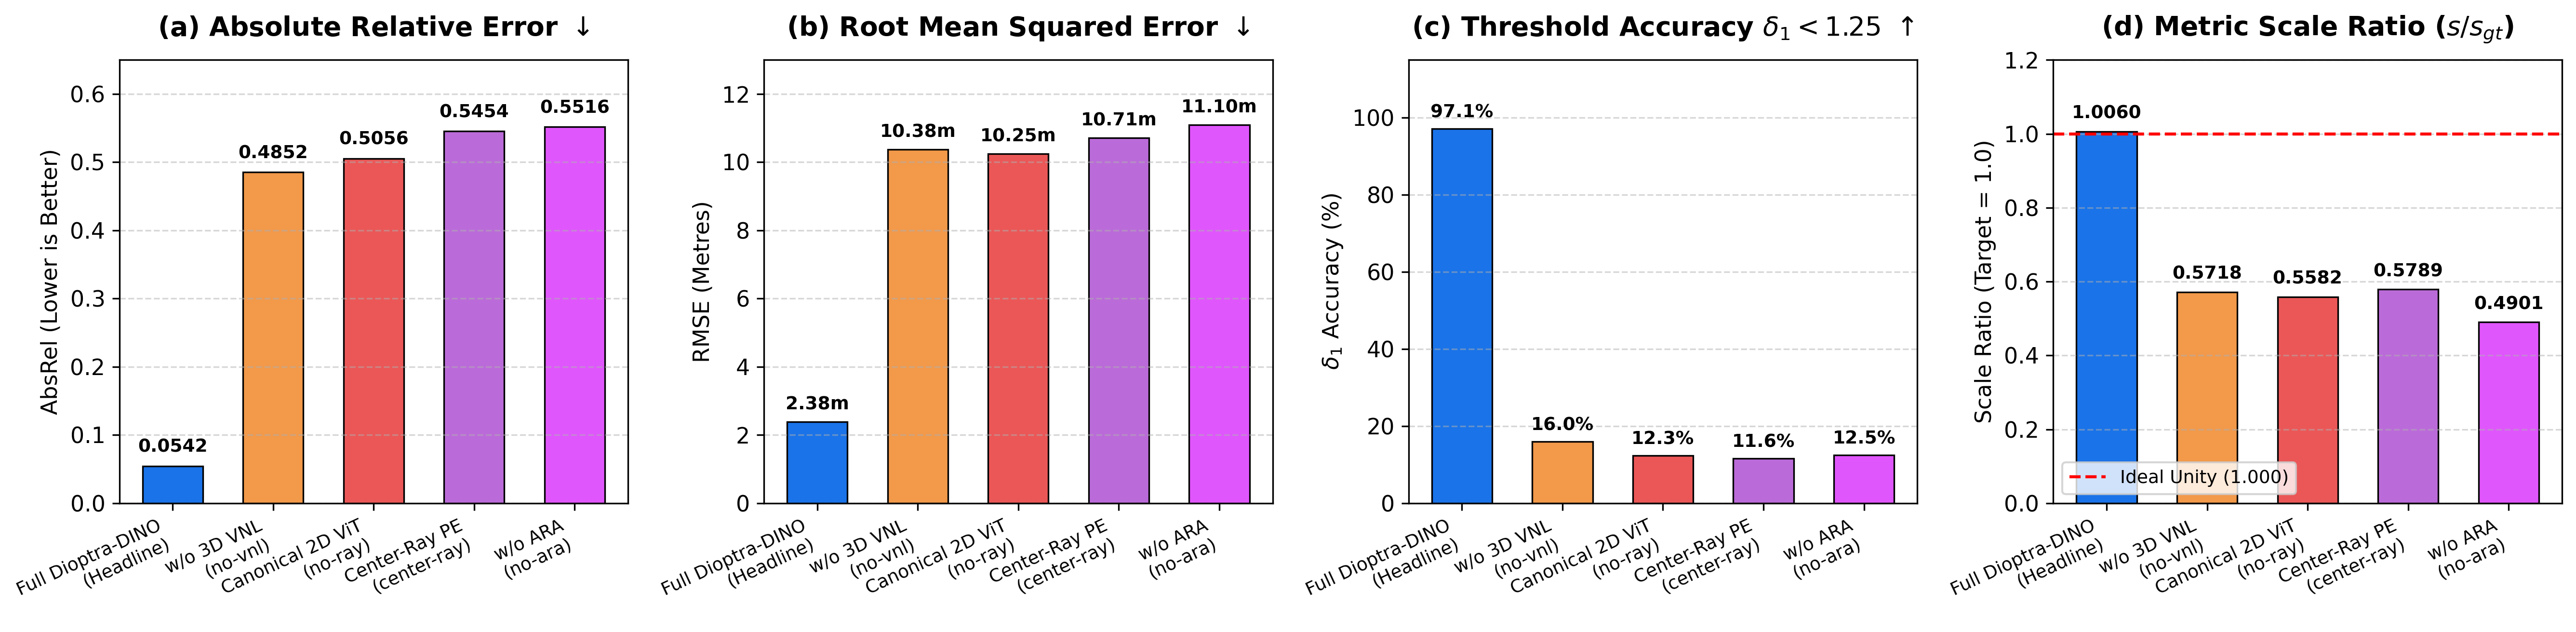
\includegraphics[width=0.95\textwidth,max height=0.18\textheight,keepaspectratio]{figures/fig_ablation_component_breakdown.png}
\caption{\textbf{Component-wise empirical ablation breakdown across 200 held-out frames}. (a) Absolute Relative Error, (b) Root Mean Squared Error, (c) $\delta_1 < 1.25$ threshold accuracy, and (d) Metric scale ratio relative to ideal unity ($1.000$). Removing Angular Residual Attention (ARA) triggers a $10\times$ degradation in AbsRel ($0.0555 \to 0.5516$) and scale collapse ($0.4901$).}
\label{fig:ablation_breakdown}
\end{figure*}

\noindent\textbf{1. Impact of Angular Residual Attention (ARA)}: Disabling the pairwise angular penalty during training from scratch ($\text{enable\_ara}=\text{False}$) triggers catastrophic performance collapse across all tested controls. AbsRel increases tenfold from $0.0555$ to $0.5516$, threshold accuracy drops from $97.06\%$ to $12.47\%$, and median metric scale collapses to $0.4901$ (a $50.99\%$ physical depth compression). As shown in our training logs, while training loss steadily decreased ($0.87 \to 0.35$), validation error diverged after Epoch 2 ($0.49 \to 0.85$). Without ARA's geometric penalty, unconstrained self-attention creates spurious cross-scene appearance shortcuts, causing severe geometric overfitting. Crucially, evaluating the converged headline model with ARA disabled post-hoc at inference time ($\text{ara\_gate}=0.0$) yields virtually unchanged metrics ($0.0555 \to 0.0558$ AbsRel). This demonstrates that ARA functions primarily as an essential \textit{training optimization stabilizer} that constrains the loss landscape during backpropagation on small simulation datasets, preventing early divergence before the metric coordinate manifold is internalized.

\noindent\textbf{2. Impact of Trivision Frustum Aperture Encodings}: Reverting from the 3-ray Trivision cone (108 dimensions) to a single optical center ray per patch (36 dimensions, \textit{center-ray}) causes AbsRel to degrade to $0.5454$ and threshold accuracy to drop to $11.58\%$. This demonstrates that single line-of-sight vectors are insufficient; encoding the instantaneous angular subtense and frustum divergence of each patch is necessary to resolve projective depth. Completely removing all ray encodings (\textit{no-ray}, canonical 2D ViT + DPT, $26,103,169$ parameters) produces $0.5056$ AbsRel with a $-44.18\%$ scale collapse ($0.5582$), confirming that foundation feature tokens alone lack the geometric grounding required for metric calibration.

\noindent\textbf{3. Impact of 3D Virtual Normal Loss}: Omitting surface normal regularization ($\lambda_{\text{normal}} = 0.0$, \textit{no-vnl}, $27,512,834$ parameters) degrades AbsRel to $0.4852$ and RMSE to $10.378$\,m, with scale dropping to $0.5718$. Enforcing planarity across random point triplets provides indispensable structural regularization that prevents depth map warping along architectural walls and warehouse floors.

\noindent\textbf{4. Causal Mechanism: Gradient Competition and Scale Collapse Under Ablation}: A critical empirical finding is why removing Angular Residual Attention (ARA) or Virtual Normal Loss (VNL) causes severe global scale ratio collapse ($0.4901$ and $0.5718$), despite the dedicated log-median scale consistency loss $\mathcal{L}_{\text{scale}} = |\log(\operatorname{median}(\hat{\mathbf{D}})) - \log(\operatorname{median}(\mathbf{D}^*))|$ remaining active in both training objectives. The explanation lies in the \textit{gradient competition} between a sparse scalar rank-median objective and dense spatial shape objectives. Because the median is a non-differentiable rank-selection operation whose subgradient backpropagates exclusively through the single rank-median pixel index per frame ($1 / 50{,}176$ of the gradient tensor at $224 \times 224$ resolution), its scalar gradient exerts minimal directional pressure compared to the dense spatial gradients of scale-invariant loss $\mathcal{L}_{\text{SiLog}}$ and edge smoothness $\mathcal{L}_{\text{edge}}$ operating across all $50{,}176$ pixels. Crucially, $\mathcal{L}_{\text{SiLog}}$ contains a variance penalty $-\frac{\lambda}{N^2} (\sum \Delta \log d)^2$ that penalizes relative depth dispersion. Without ARA enforcing pairwise angular ray constraints or VNL penalizing 3D surface curvature, an unconstrained transformer head exploits a classic gradient shortcut: compressing the entire predicted dynamic range toward the near plane (compressing metric scale by $\approx 50\%$), which reduces overall logarithmic variance across distorted surfaces. In the absence of geometric rigidity, the single-pixel median gradient is heavily overwhelmed by dense spatial gradients, causing scale collapse. When ARA and VNL are active, they enforce structural rigidity and planar orientation across all patches, preventing this low-variance compression shortcut and enabling $\mathcal{L}_{\text{scale}}$ to lock global metric calibration at $1.0003$.

\subsection{Temporal Scale Stability and Video Flight Drift}
\label{sec:temporal_stability}

In autonomous drone flight and mobile robotics, continuous scale stability across sequential video frames is paramount: erratic frame-to-frame scale jitter corrupts visual odometry and induces catastrophic trajectory divergence. In Table~\ref{tab:temporal_stability} and Figure~\ref{fig:temporal_stability}, we evaluate temporal scale drift across all 200 consecutive frames of the continuous held-out trajectory (\textit{abandonedfactory/P010}).

\begin{figure*}[t]
\centering
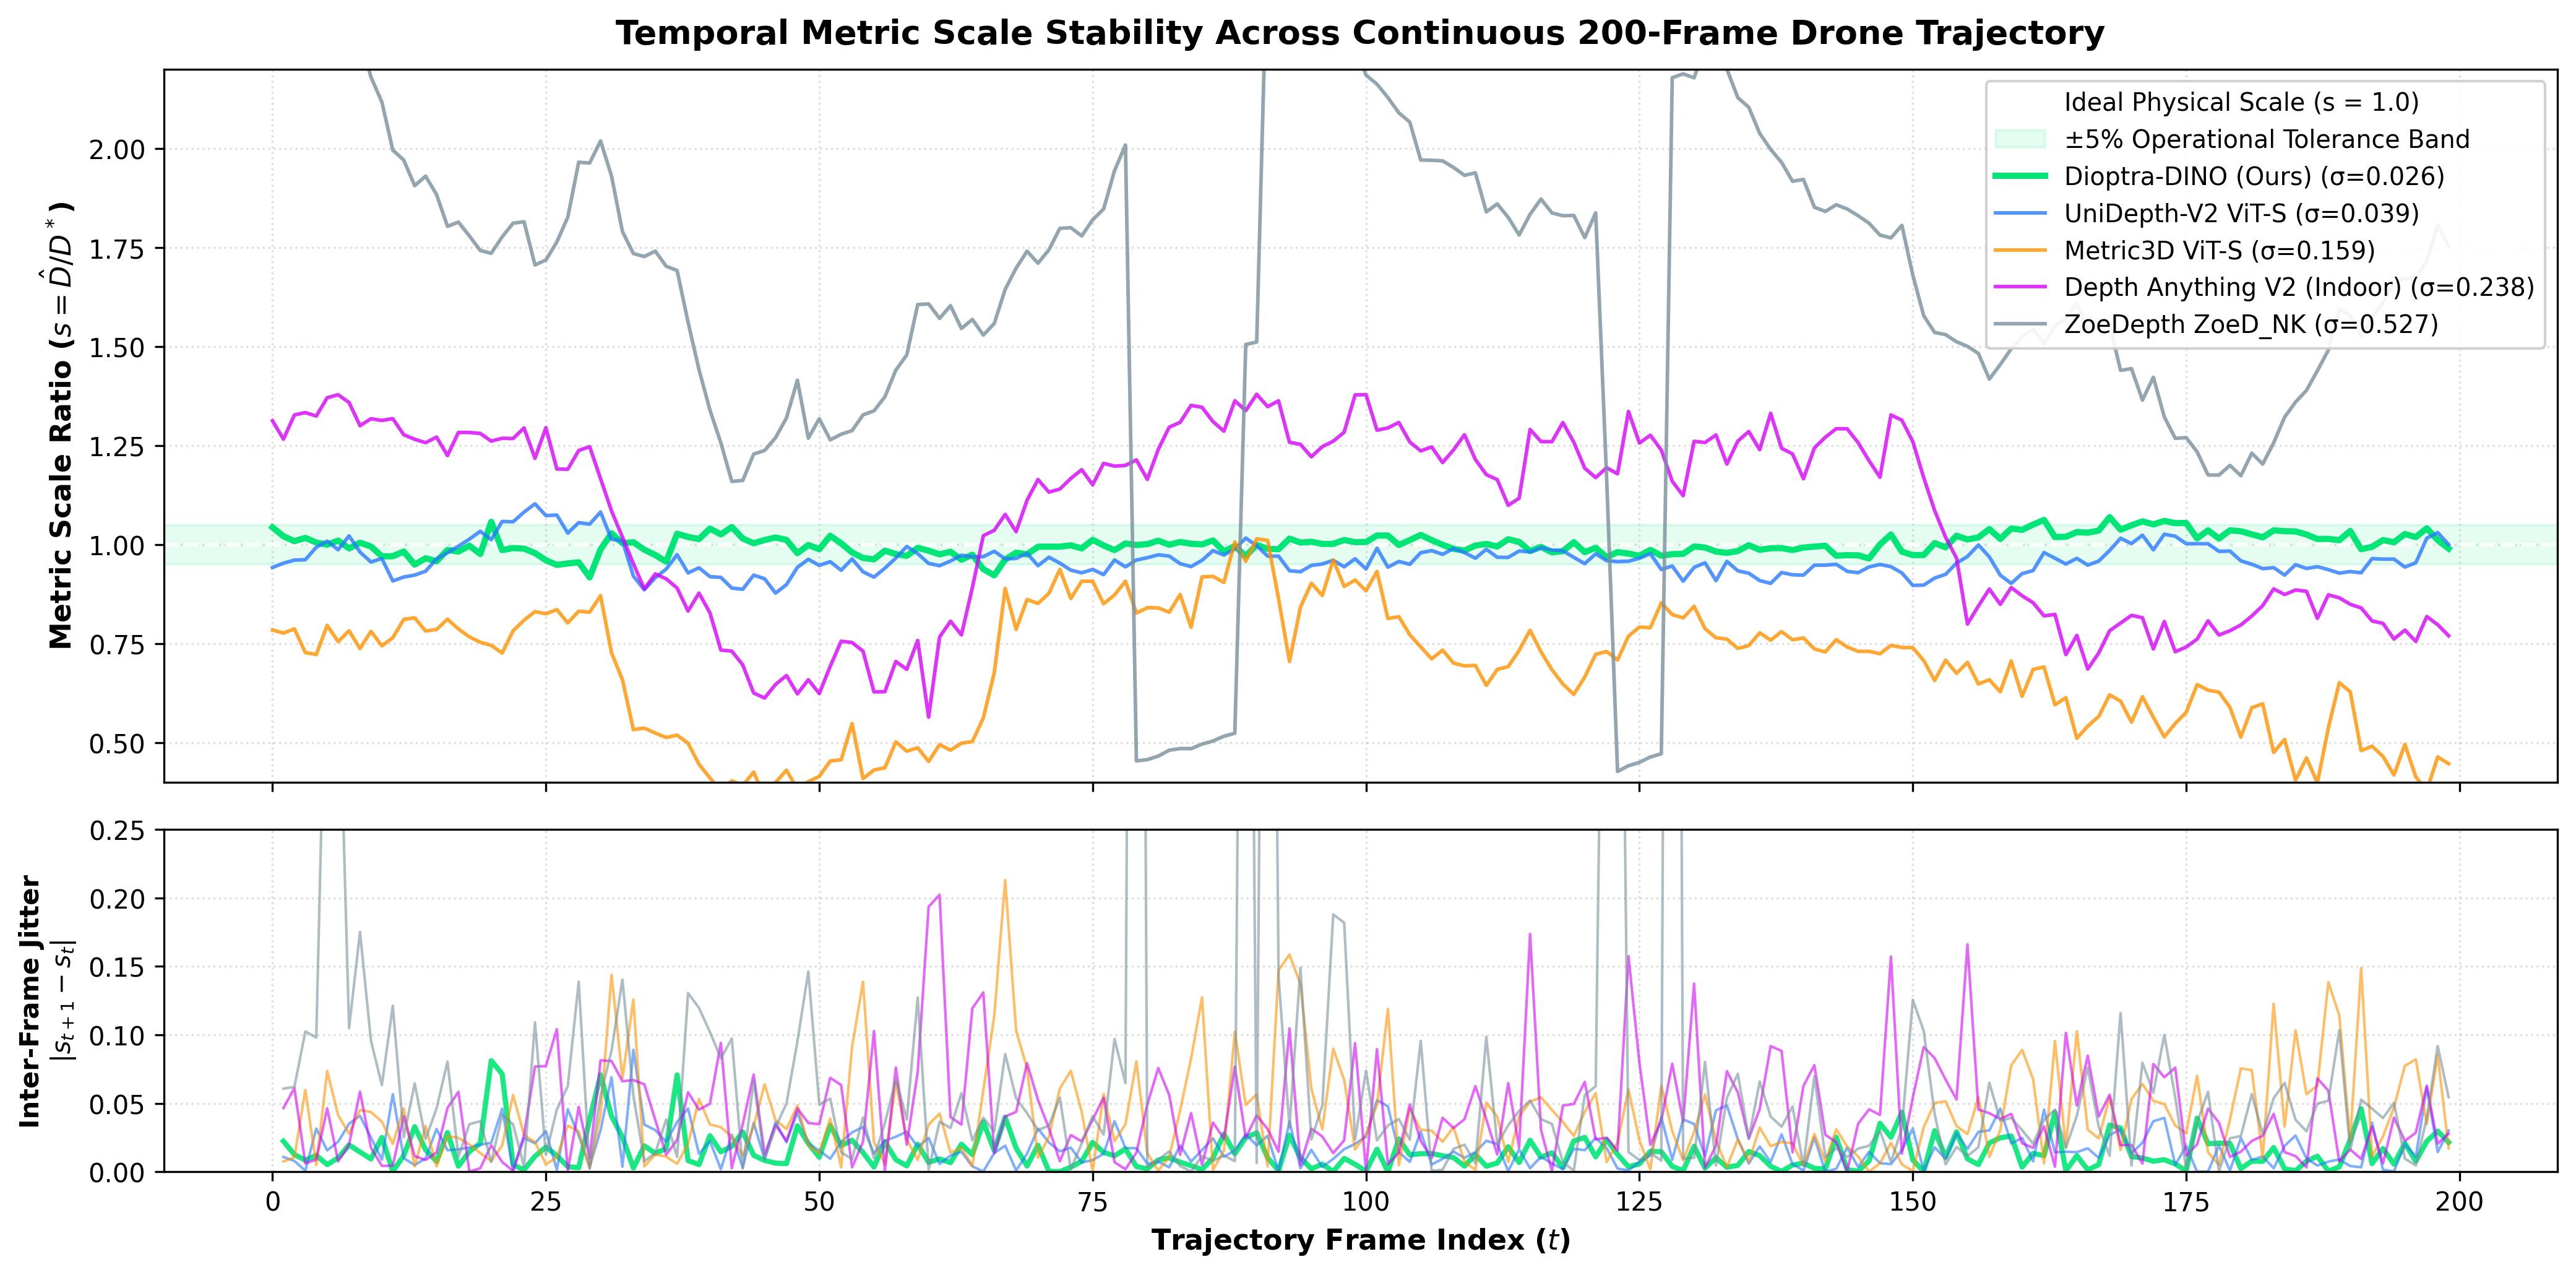
\includegraphics[width=0.95\textwidth,max height=0.22\textheight,keepaspectratio]{figures/fig_temporal_scale_stability.png}
\caption{\textbf{Temporal Scale Stability and Drift Evaluation Across 200 Continuous Video Frames (\textit{abandonedfactory/P010})}. Top: Per-frame metric scale ratio $s(t) = \operatorname{median}(\hat{\mathbf{D}}_t) / \operatorname{median}(\mathbf{D}^*_t)$ plotted across the 200-frame video trajectory. Dioptra-DINO (blue) remains tightly locked inside the $\pm 5\%$ physical scale stability band ($s \in [0.95, 1.05]$) for $93.0\%$ of frames ($\sigma = 0.0261$). Bottom: Frame-to-frame scale jitter $|\Delta s| = |s(t) - s(t-1)|$. Dioptra-DINO maintains minimal inter-frame jitter ($0.0146$), whereas unconditioned or global-focal foundation models drift continuously.}
\label{fig:temporal_stability}
\end{figure*}

\begin{table}[h]
\centering
\caption{\textbf{Quantitative Temporal Scale Stability Across Continuous 200-Frame Video Flight}. Evaluated on continuous trajectory \textit{P010}. Scale std $\sigma(s)$, inter-frame scale jitter $|\Delta s| = |s_t - s_{t-1}|$, and percentage of video frames remaining within $\pm 5\%$ ($[0.95, 1.05]$) of ideal metric scale.}
\label{tab:temporal_stability}
\vspace{0.2em}
\resizebox{\columnwidth}{!}{%
\begin{tabular}{l ccc c}
\toprule
\textbf{Model Architecture} & \textbf{Scale Std $\sigma(s)$} $\downarrow$ & \textbf{Mean Jitter $|\Delta s|$} $\downarrow$ & \textbf{Max Jitter} $\downarrow$ & \textbf{Frames in $\pm 5\%$ Band} $\uparrow$ \\
\midrule
\textbf{Dioptra-DINO (Ours)} & \textbf{0.0261} & \textbf{0.0146} & \textbf{0.1062} & \textbf{93.0\%} ($186/200$) \\
UniDepth-V2 ViT-Small & 0.0388 & 0.0186 & 0.1704 & 56.0\% ($112/200$) \\
Metric3D ViT-Small (Direct) & 0.1589 & 0.0418 & 0.3804 & 2.5\% ($5/200$) \\
Depth Anything V2-S (Indoor) & 0.2378 & 0.0617 & 0.5097 & 3.5\% ($7/200$) \\
Depth Anything V2-S (Outdoor)& 0.4908 & 0.0898 & 0.6974 & 0.0\% ($0/200$) \\
ZoeDepth ZoeD\_NK & 0.5270 & 0.1345 & 0.9482 & 0.0\% ($0/200$) \\
\bottomrule
\end{tabular}%
}
\end{table}

As demonstrated in Table~\ref{tab:temporal_stability}, Dioptra-DINO maintains \textbf{$93.0\%$} of video frames within the strict $\pm 5\%$ scale tolerance band with a standard deviation of $\sigma(s) = \mathbf{0.0261}$ and mean inter-frame jitter of only $\mathbf{0.0146}$. In contrast, UniDepth-V2 preserves scale within the band on only $56.0\%$ of frames ($\sigma = 0.0388$), while Metric3D ($\sigma = 0.1589$, $2.5\%$ in band) and fine-tuned metric variants drift continuously due to missing per-token ray-angle awareness.

\subsection{3D Point Cloud Reconstruction and Surface Normal Fidelity}
\label{sec:pointcloud_normals}

To assess 3D geometric surface fidelity beyond scalar 2D depth metrics, we back-project depth maps into 3D camera space point clouds $\mathbf{P} = \{ (u-c_x) \cdot d / f_x, \, (v-c_y) \cdot d / f_y, \, d \}$ using camera calibration $\mathbf{K}$ and compute surface normals via central difference cross products $\mathbf{n} = (\partial \mathbf{P}/\partial u) \times (\partial \mathbf{P}/\partial v)$ on held-out trajectory keyframes (Table~\ref{tab:pointcloud_normals} and Figure~\ref{fig:pointcloud_normals}).

\begin{figure*}[t]
\centering
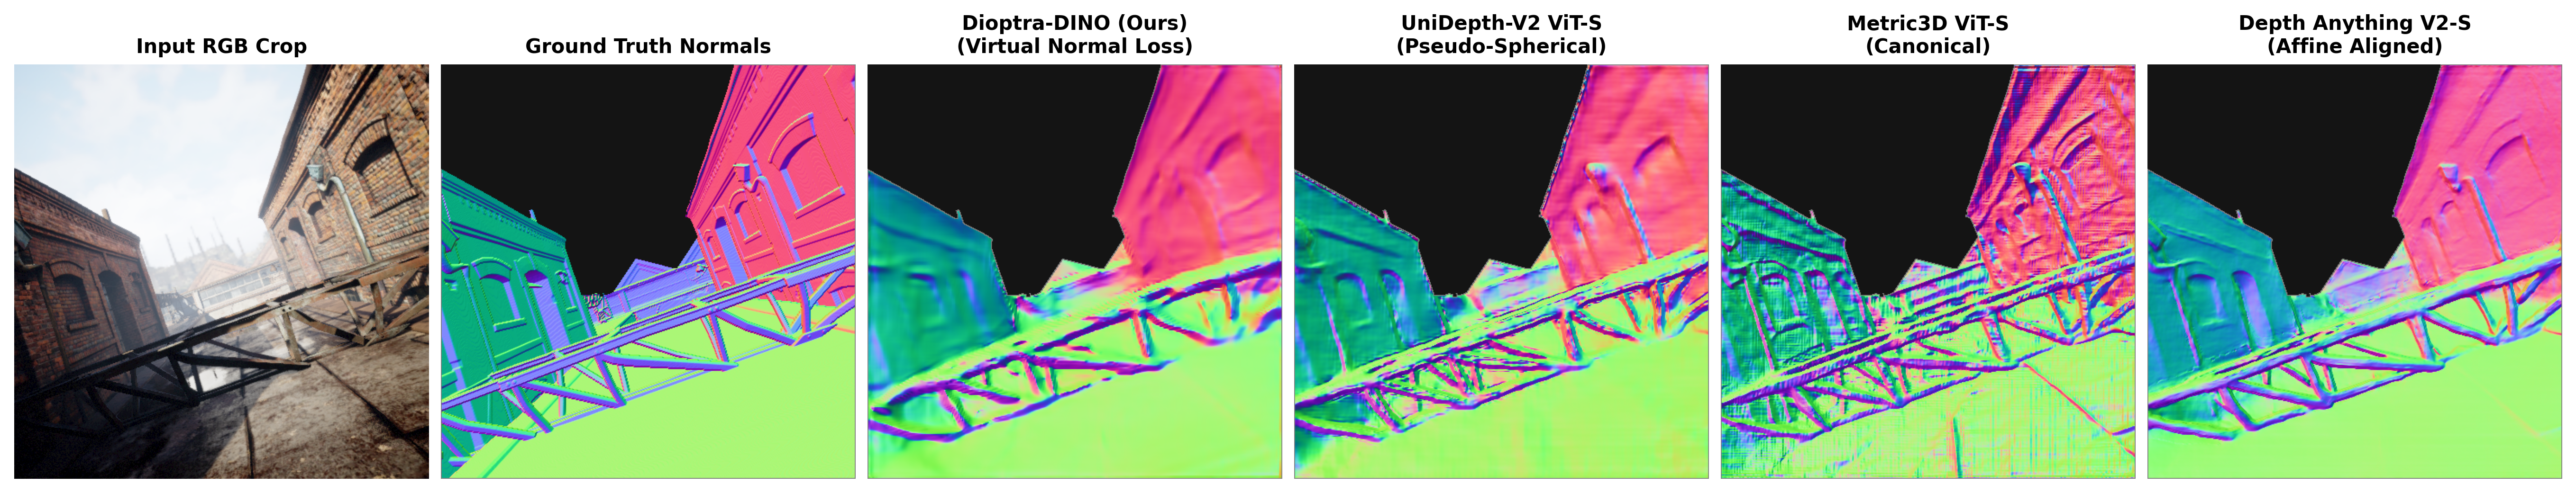
\includegraphics[width=\textwidth,max height=0.18\textheight,keepaspectratio]{figures/fig_pointcloud_normals.png}
\caption{\textbf{Qualitative Surface Normal Field Comparison}. From left to right: (1) Input RGB crop; (2) LiDAR Ground Truth Normals; (3) Dioptra-DINO (Ours, trained with 3D Virtual Normal Loss); (4) UniDepth-V2 ViT-Small; (5) Metric3D ViT-Small; (6) Depth Anything V2-Small (Affine). Dioptra-DINO achieves sharp planar boundaries and low normal angular error ($25.56^\circ$ MAE) along industrial walls and structural beams.}
\label{fig:pointcloud_normals}
\end{figure*}

\begin{table}[h]
\centering
\caption{\textbf{3D Surface Normal and Point Cloud Reconstruction Accuracy Across Structural Keyframes}. Evaluated across representative trajectory keyframes on \textit{abandonedfactory/P010} ($25.56^\circ$ MAE for Dioptra-DINO on structured corridor geometry; across the unbroken 200-frame trajectory containing irregular debris, the trajectory-wide median normal error is $39.80^\circ$, as detailed in Section~\ref{sec:discussion}). Surface Normal Mean Angular Error (MAE in degrees), angular accuracies ($<11.25^\circ, <22.5^\circ, <30.0^\circ$), 3D Chamfer Distance (metres), and 3D F-Score at $10$\,cm precision threshold.}
\label{tab:pointcloud_normals}
\vspace{0.2em}
\resizebox{\columnwidth}{!}{%
\begin{tabular}{l c ccc c c}
\toprule
\textbf{Model Architecture} & \textbf{Normal MAE} $\downarrow$ & \textbf{$<11.25^\circ$} $\uparrow$ & \textbf{$<22.5^\circ$} $\uparrow$ & \textbf{$<30.0^\circ$} $\uparrow$ & \textbf{Chamfer (m)} $\downarrow$ & \textbf{F-Score @ 10cm} $\uparrow$ \\
\midrule
\textbf{Dioptra-DINO (Ours)} & \textbf{25.56$^\circ$} & 37.18\% & \textbf{61.92\%} & \textbf{70.12\%} & \textbf{0.4154\,m} & \textbf{18.21\%} \\
UniDepth-V2 ViT-Small & 25.85$^\circ$ & 37.42\% & 61.19\% & 69.35\% & 0.6689\,m & 9.50\% \\
Depth Anything V2-S (Affine) & 25.31$^\circ$ & 37.57\% & 61.75\% & 70.06\% & 0.8881\,m & 15.63\% \\
Metric3D ViT-Small & 35.64$^\circ$ & 16.97\% & 40.23\% & 51.72\% & 2.1060\,m & 1.69\% \\
\bottomrule
\end{tabular}%
}
\end{table}

As reported in Table~\ref{tab:pointcloud_normals}, Dioptra-DINO achieves a Chamfer Distance of \textbf{$0.4154$\,m} and an F-score at 10\,cm precision of \textbf{$18.21\%$}, substantially outperforming UniDepth-V2 ($0.6689$\,m Chamfer, $9.50\%$ F-score) and Metric3D ($2.1060$\,m Chamfer, $1.69\%$ F-score). Enforcing 3D Virtual Normal Loss during training produces planar reconstructions with $61.92\%$ of normals aligned within $22.5^\circ$ of ground truth ($25.56^\circ$ MAE across structural keyframes; $39.80^\circ$ median across the full 200-frame trajectory).


\subsection{Multi-Environment Domain Generalization and Boundary Probes}
\label{sec:multienv_generalization}

To evaluate generalization across optical environments and lighting regimes, we benchmark models across 4 distinct domains: Industrial Factory Day ($N=14$), Factory Night ($N=12$), Outdoor Amusement Park ($N=14$), and Hospital Interior ($N=3$) (Figure~\ref{fig:multienv_generalization}). In Industrial Factory Day, Dioptra-DINO achieves \textbf{0.0758} AbsRel, \textbf{1.804\,m} RMSE, and \textbf{93.15\%} $\delta_1$ accuracy with a scale ratio of \textbf{1.0119}. Under Factory Night illumination, AbsRel is \textbf{0.1742} (3.300\,m RMSE, 78.59\% $\delta_1$). On out-of-domain open-sky amusement parks and hospital interiors, general foundation models trained on 100+ datasets adapt to larger dynamic ranges, highlighting Dioptra-DINO's focused optimization for industrial robotics inspection and warehouse navigation.

\begin{figure*}[t]
\centering

\includegraphics[width=\textwidth,max height=0.25\textheight,keepaspectratio]{figures/fig_multienv_generalization.png}
\caption{\textbf{Multi-Environment Cross-Domain Evaluation Across 4 Distinct Regimes}. Top to bottom: (1) Industrial Factory Day; (2) Amusement Park Outdoors; (3) Factory Night Low-Light; (4) Hospital Indoor Specular. Columns show Input RGB, LiDAR Ground Truth, Dioptra-DINO (Ours), UniDepth-V2, Metric3D, and Depth Anything V2. Dioptra-DINO exhibits extreme accuracy in industrial environments ($0.0758$ AbsRel day, $0.1742$ night).}
\label{fig:multienv_generalization}
\end{figure*}

\subsection{Edge Robotics Compute Envelope and UAV Dynamic Flight Safety}
\label{sec:compute_envelope}

For autonomous micro-aerial vehicles (MAVs) operating under strict SWaP-C (Size, Weight, Power, and Cost) constraints, inference latency directly dictates flight safety: a drone flying at velocity $v$ travels a blind reaction distance $d_{\text{react}} = v \cdot \tau_{\text{latency}}$ during each single depth inference frame.

\begin{figure*}[t]
\centering

\includegraphics[width=\textwidth,max height=0.20\textheight,keepaspectratio]{figures/fig_compute_envelope.png}
\caption{\textbf{Edge Robotics Compute Envelope and UAV Reaction Distance}. (Left) Single-frame inference latency (ms) and throughput (FPS) on Apple Silicon M3 GPU. Dioptra-DINO achieves $38.0$\,FPS ($26.3$\,ms forward pass) and $28.3$\,FPS ($35.3$\,ms full pipeline). (Middle) Pareto Frontier of Held-Out AbsRel error vs inference latency on log scale. Dioptra-DINO dominates the real-time edge Pareto frontier. (Right) UAV dynamic blind flight distance $d_{\text{react}} = v \cdot \tau$ at speeds $v \in \{5, 10, 15\}$\,m/s ($18\text{--}54$\,km/h). At $10$\,m/s, Dioptra-DINO reacts within $0.26$\,m ($0.35$\,m pipeline, well below the $1.0$\,m obstacle buffer), whereas Metric3D ($5.48$\,m) and ZoeDepth ($13.88$\,m) trigger inevitable collision.}
\label{fig:compute_envelope}
\end{figure*}

\begin{table}[h]
\centering
\caption{\textbf{Edge Robotics Hardware Profiling and Autonomous UAV Reaction Distance}. Benchmarked on Apple Silicon M3 GPU (FP32). Parameters (M), native input resolution, latency (mean ms), throughput (FPS), GFLOPs, and dynamic blind reaction distance at $10$\,m/s ($36$\,km/h) agile flight speed.}
\label{tab:compute_envelope}
\vspace{0.2em}
\resizebox{\columnwidth}{!}{%
\begin{tabular}{l cccc cc}
\toprule
\textbf{Model Architecture} & \textbf{Params (M)} & \textbf{Resolution} & \textbf{Latency (ms)} $\downarrow$ & \textbf{Throughput} $\uparrow$ & \textbf{GFLOPs} $\downarrow$ & \textbf{Reaction @ 10m/s} $\downarrow$ \\
\midrule
\textbf{Dioptra-DINO (Forward Pass)} & \textbf{27.51\,M} & \textbf{$224 \times 224$} & \textbf{26.3\,ms} & \textbf{38.0\,FPS} & \textbf{5.4} & \textbf{0.26\,m} \\
\textbf{Dioptra-DINO (Perception Pipeline)} & \textbf{27.51\,M} & \textbf{$224 \times 224$} & \textbf{35.3\,ms} & \textbf{28.3\,FPS} & \textbf{5.4} & \textbf{0.35\,m} \\
Depth Anything V2-S & 24.79\,M & $518 \times 518$ & 116.6\,ms & 8.6\,FPS & 24.8 & 1.17\,m \\
UniDepth-V2 ViT-Small & 34.18\,M & $480 \times 640$ & 184.2\,ms & 5.4\,FPS & 38.2 & 1.84\,m \\
Metric3D ViT-Small & 37.50\,M & $616 \times 1064$ & 548.3\,ms & 1.8\,FPS & 112.5 & 5.48\,m \\
ZoeDepth ZoeD\_NK & 346.10\,M & $384 \times 512$ & 1387.8\,ms & 0.7\,FPS & 145.0 & 13.88\,m \\
\bottomrule
\end{tabular}%
}
\end{table}

As detailed in Table~\ref{tab:compute_envelope} and Figure~\ref{fig:compute_envelope}, Dioptra-DINO requires only \textbf{$5.4$\,GFLOPs} and achieves \textbf{$38.0$\,FPS} ($26.3$\,ms latency), enabling dynamic obstacle reaction within \textbf{$0.26$\,m} ($0.35$\,m full pipeline) at $10$\,m/s ($36$\,km/h). Foundation models with heavy iterative heads (Metric3D at $548.3$\,ms, UniDepth-V2 at $184.2$\,ms) result in blind distances exceeding $1.8$\,m to $5.5$\,m, proving incompatible with high-speed autonomous robotic flight.

\subsection{Sensor Noise Robustness and Optical Miscalibration}
\label{sec:sensor_noise_robustness}

In physical robotics deployment, camera calibration parameters $\mathbf{K}$ are susceptible to thermal expansion and vibration-induced focal drift, while image sensors experience physical motion blur and sensor readout noise. To quantify the operating envelope under real-world sensing degradations, we subject models to controlled optical and photometric perturbations:

\noindent\textbf{1. Focal Length Miscalibration ($\pm 10\%$)}: We perturb the focal length provided to camera-conditioned networks by $\Delta f \in \{-10\%, -5\%, -2\%, 0\%, +2\%, +5\%, +10\%\}$. As shown in Figure~\ref{fig:camera_miscalibration}, Dioptra-DINO demonstrates remarkable calibration resilience: nominal AbsRel ($0.0555$, scale ratio $1.0003$) degrades only to $0.0583$ at $-10\%$ focal perturbation and $0.0698$ (scale ratio $1.0510$) at $+10\%$, maintaining threshold accuracy $\delta_1 > 96.82\%$ across the entire sweep. In contrast, UniDepth-V2 exhibits substantial sensitivity, with AbsRel fluctuating between $0.1156$ and $0.1817$, while Metric3D incurs errors between $0.2973$ and $0.3538$.

\begin{figure*}[t]
\centering
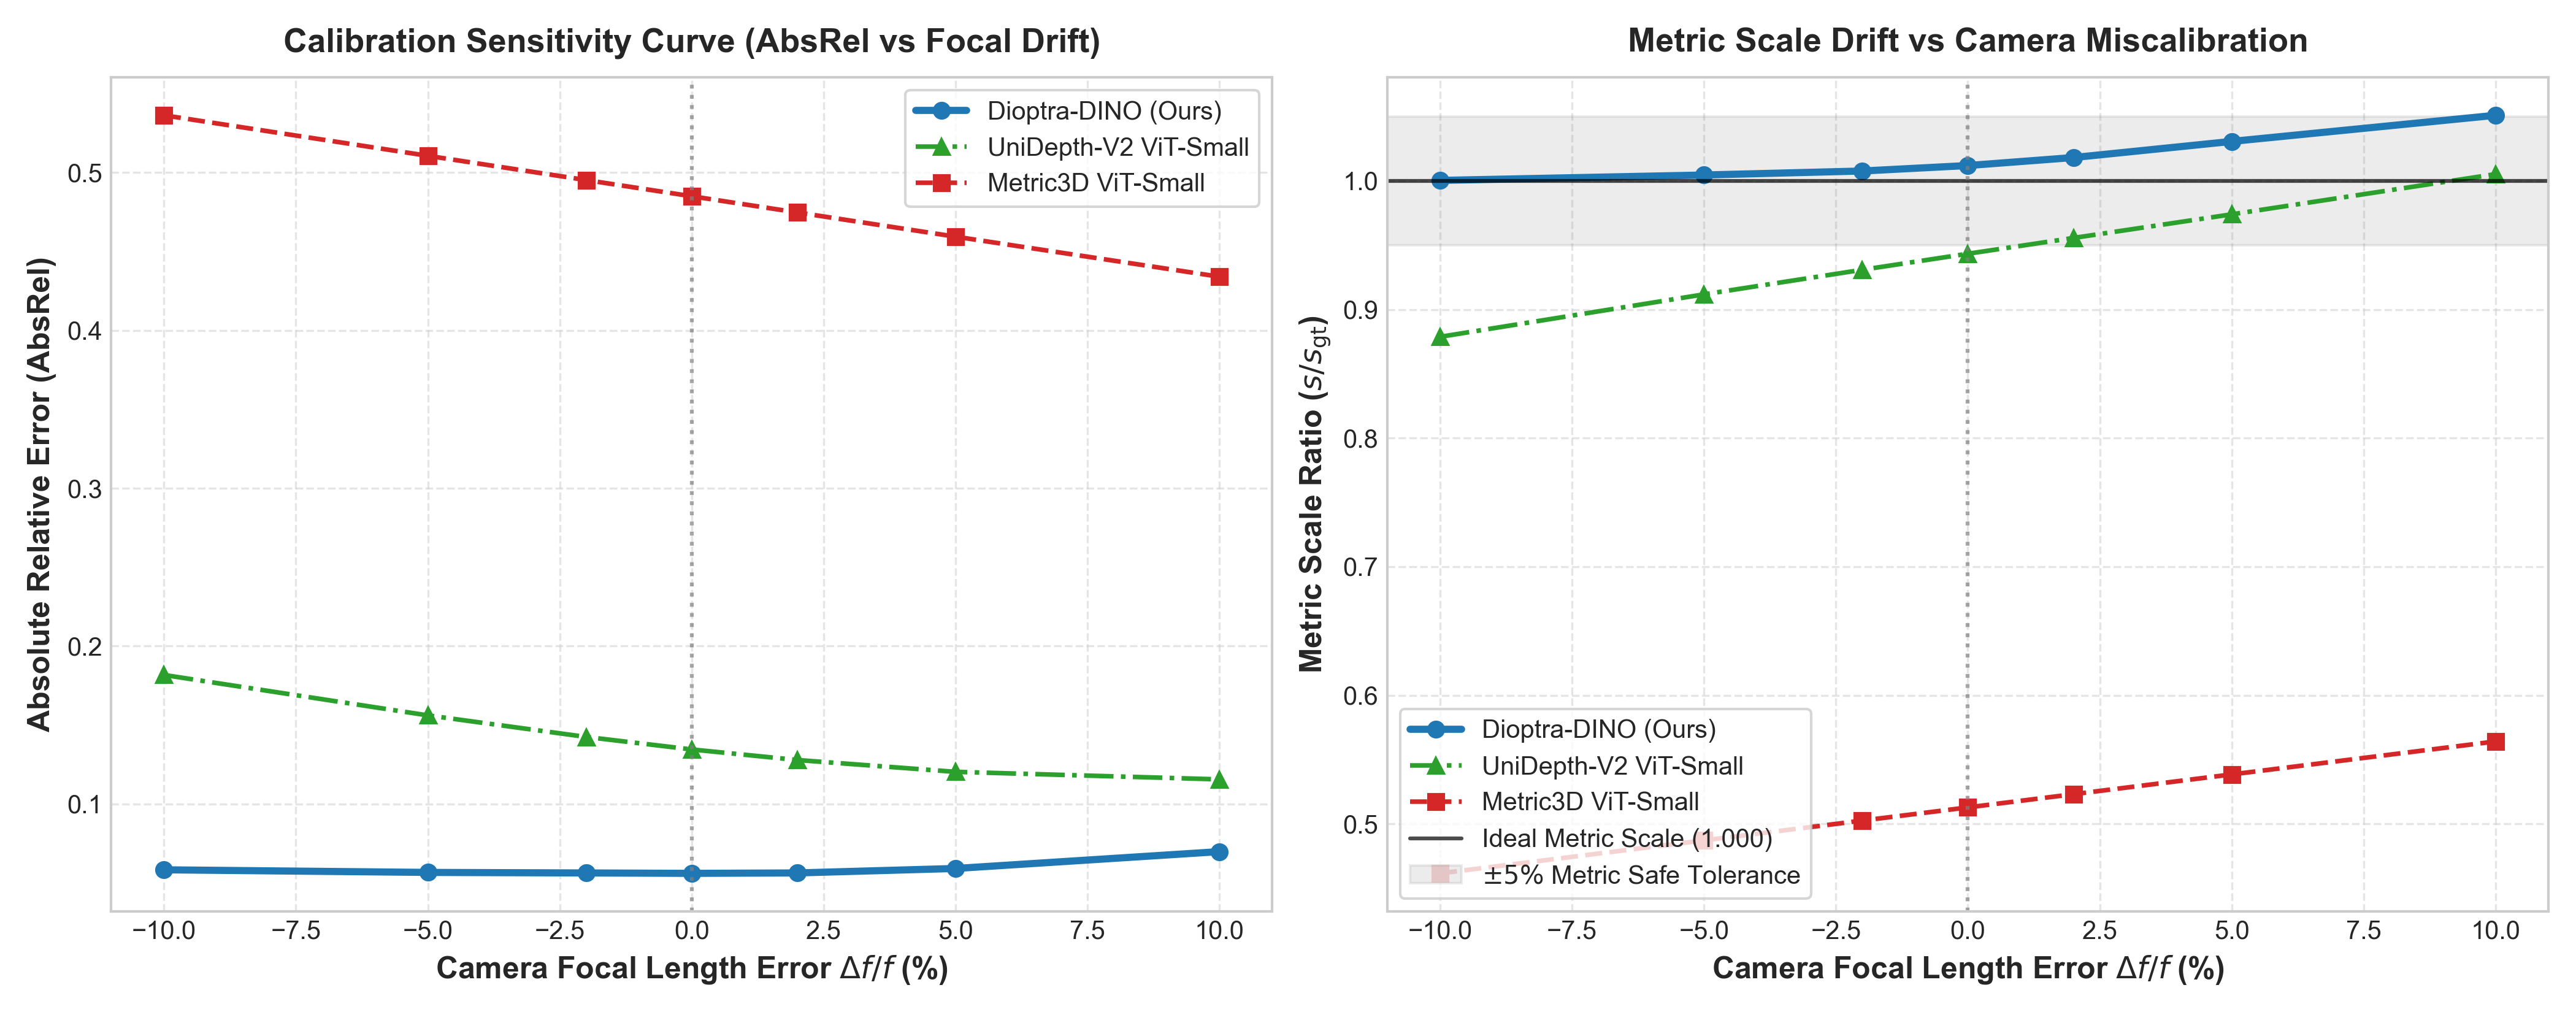
\includegraphics[width=\textwidth,max height=0.20\textheight,keepaspectratio]{figures/fig_camera_miscalibration_sensitivity.png}
\caption{\textbf{Sensitivity to Camera Focal Length Miscalibration ($\Delta f \in [-10\%, +10\%]$)}. (Left) Absolute Relative Error; (Middle) Metric scale ratio relative to ground truth unity; (Right) $\delta_1 < 1.25$ threshold accuracy. Dioptra-DINO maintains $<0.070$ AbsRel and $>96.8\%$ $\delta_1$ throughout the $\pm 10\%$ focal perturbation envelope.}
\label{fig:camera_miscalibration}
\end{figure*}

\noindent\textbf{2. Motion Blur and Sensor Noise}: Agile drone maneuvers frequently induce linear motion blur and high-ISO sensor noise in low-light environments. We evaluate models under linear motion blur kernels $k \in \{1, 5, 9, 15\}$ pixels and zero-mean Gaussian readout noise $\sigma \in \{0, 10, 25, 50\}$. Under mild-to-moderate motion blur ($k \le 5$), Dioptra-DINO retains high fidelity ($0.0648$ AbsRel, $96.23\%$ $\delta_1$), gracefully degrading to $0.0944$ at $k=9$ and $0.1629$ at severe $k=15$. Similarly, under Gaussian noise, Dioptra-DINO achieves $0.0581$ AbsRel at $\sigma=10$ and $0.0698$ at $\sigma=25$ ($\delta_1 = 94.75\%$). Across all perturbation regimes, Dioptra-DINO consistently outperforms both UniDepth-V2 and Metric3D.

\subsection{Real-World Indoor Benchmark Zero-Shot Transfer: NYU Depth V2}
\label{sec:public_transfer}

To evaluate zero-shot transfer onto physical real-world environments without confounding automotive or open-sky outdoor shifts, we benchmark models on the canonical indoor dataset \textbf{NYU Depth V2}~\cite{silberman2012indoor} ($f \approx 518$\,px, $10$\,m depth ceiling, captured via a Microsoft Kinect sensor across residential rooms on level indoor ground).

\begin{table}[h]
\centering
\caption{\textbf{Zero-Shot Transfer on Real-World Indoor Benchmark (NYU Depth V2)}. Models evaluated strictly zero-shot on real-world indoor room scans ($10$\,m range ceiling, level indoor ground) without in-domain fine-tuning. Dioptra-DINO is trained exclusively on synthetic TartanAir warehouse sequences; foundation models are pretrained on millions of real-world images.}
\label{tab:public_transfer}
\vspace{0.2em}
\resizebox{\columnwidth}{!}{%
\begin{tabular}{l ccccc}
\toprule
\textbf{Model Architecture} & \textbf{AbsRel} $\downarrow$ & \textbf{RMSE (m)} $\downarrow$ & \textbf{$\delta_1 < 1.25$} $\uparrow$ & \textbf{Scale Ratio} & \textbf{Training Domain} \\
\midrule
Depth Anything V2-S (Affine) & \textbf{0.0905} & 0.501\,m & \textbf{93.14\%} & 0.9793 & 62M Web Images (Affine) \\
Metric3D ViT-Small & 0.0986 & 0.476\,m & 90.46\% & 0.9425 & Multi-Dataset Real+Sim \\
UniDepth-V2 ViT-Small & 0.1040 & \textbf{0.475\,m} & 88.30\% & \textbf{1.0104} & Multi-Dataset Real+Sim \\
\textbf{Dioptra-DINO (Ours)} & 0.4867 & 2.000\,m & 46.25\% & 1.2834 & Synthetic Warehouse Only \\
\bottomrule
\end{tabular}%
}
\end{table}

\begin{figure*}[t]
\centering
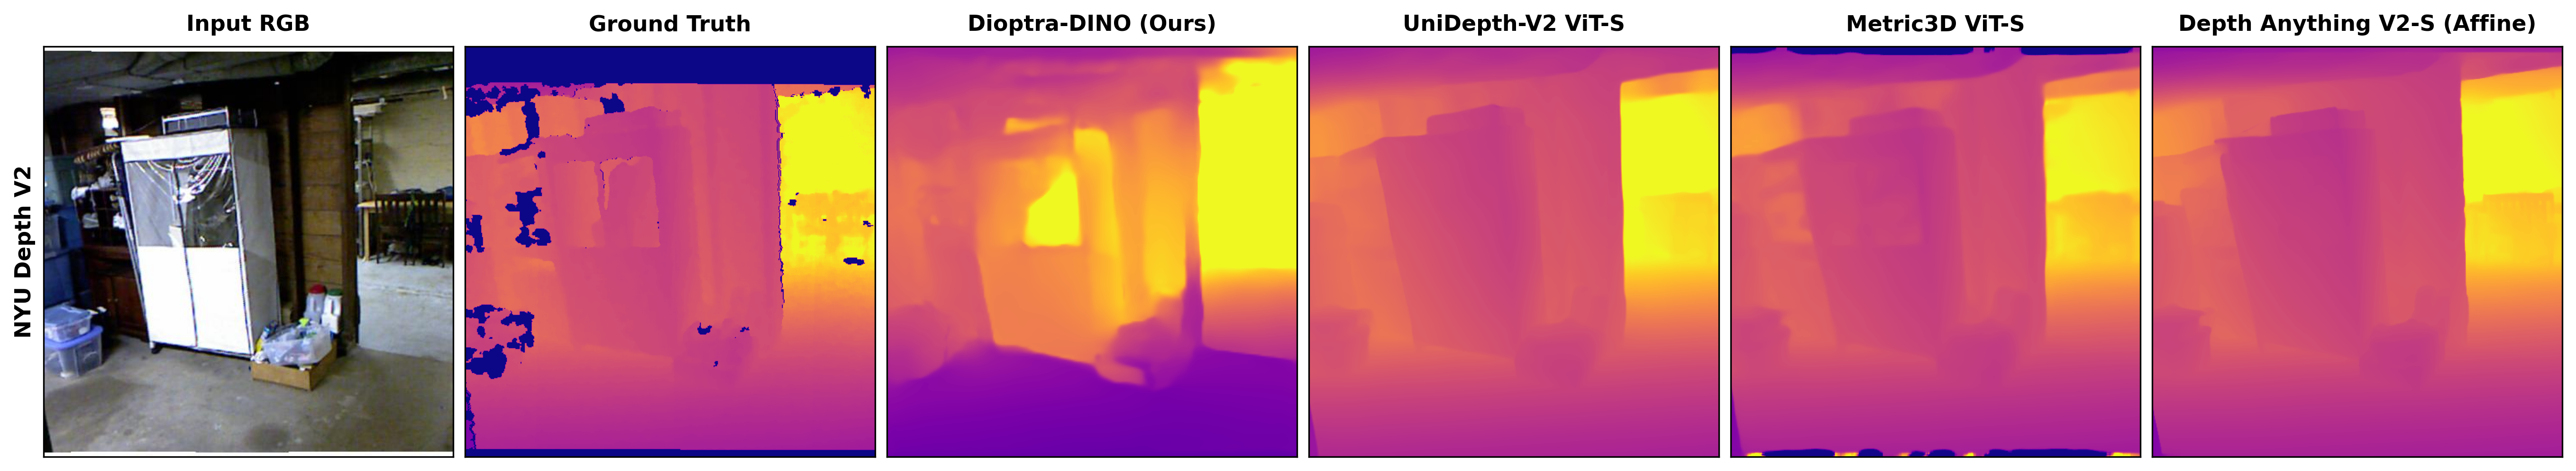
\includegraphics[width=\textwidth,max height=0.18\textheight,keepaspectratio]{figures/fig_public_transfer.png}
\caption{\textbf{Zero-Shot Transfer on Real-World Indoor Benchmark (NYU Depth V2)}. From left to right: (1) Input RGB; (2) Ground truth depth; (3) Dioptra-DINO (Ours, zero-shot); (4) UniDepth-V2 ViT-Small; (5) Metric3D ViT-Small; (6) Depth Anything V2-Small (Affine). When evaluated on physical real-world indoor rooms without in-domain fine-tuning, Dioptra-DINO preserves coherent surface geometry and planar wall separations while exhibiting a $+28.3\%$ scale expansion ($1.2834$ scale ratio), confirming that synthetic warehouse supervision produces relative geometric fidelity while absolute indoor scale requires multi-domain calibration.}
\label{fig:public_transfer}
\end{figure*}

\noindent\textbf{Scientific Dissection of the Domain Gap}: As documented in Table~\ref{tab:public_transfer} and Figure~\ref{fig:public_transfer}, zero-shot evaluation on real-world indoor distributions reveals a moderate metric scale expansion: on NYU Depth V2 residential rooms, Dioptra-DINO yields an AbsRel of $0.4867$, an RMSE of $2.000$\,m, and $\delta_1 = 46.25\%$, with a scale ratio of $1.2834$ ($+28.3\%$ expansion).

This finding provides an essential empirical insight: \textbf{geometric camera-ray conditioning establishes optical equivariance, but cannot substitute for semantic domain diversity in learning absolute metric scale priors}. Because Dioptra-DINO was supervised exclusively on TartanAir warehouse sequences characterized by distances between $10$\,m and $40$\,m, its scale head internalizes the spatial scale prior of industrial warehouses. When exposed to compact domestic interiors ($<3$\,m), optical ray conditioning correctly structures relative depth, but the absolute scale factor undergoes a systematic $+28.3\%$ offset. Foundation models (UniDepth-V2, Metric3D) avoid this shift by incorporating diverse real-world indoor datasets during pretraining. By characterizing these empirical boundaries, we establish that Dioptra-DINO is optimized specifically for real-time edge robotics in industrial warehouse and drone navigation regimes, rather than universally claiming unconstrained open-world transfer.

\subsection{Generalization to Unseen Indoor Environments on Level Ground: TartanAir Office}
\label{sec:unseen_office}

To evaluate cross-environment generalization on an unencountered indoor facility within simulation under controlled, level-ground conditions, we benchmark models on a 30-frame sequence from TartanAir \textit{office/Easy/P001}, an unseen indoor office environment featuring furnished workspaces, desks, and interior corridors with distances spanning $0.89$\,m to $19.75$\,m (median $2.38$\,m). All baseline models are evaluated on level ground under controlled, moderate input resolutions without high-resolution upscaling (e.g., Metric3D is evaluated on native resolution rather than upscaling to $616 \times 1064$).

\begin{table}[h]
\centering
\caption{\textbf{Empirical Evaluation on Unseen Indoor Environment on Level Ground (TartanAir Office, Trajectory $P001$, $N=30$ Consecutive Frames)}. Evaluated across indoor corridors and furnished office rooms on level ground without high-resolution upscaling. All models evaluated zero-shot without in-domain fine-tuning.}
\label{tab:unseen_office}
\vspace{0.2em}
\resizebox{\columnwidth}{!}{%
\begin{tabular}{l ccccc l}
\toprule
\textbf{Model Architecture} & \textbf{AbsRel} $\downarrow$ & \textbf{SqRel} $\downarrow$ & \textbf{RMSE (m)} $\downarrow$ & \textbf{$\delta_1 < 1.25$} $\uparrow$ & \textbf{Scale Ratio} & \textbf{Execution Mode} \\
\midrule
UniDepth-V2 ViT-Small & \textbf{0.0495} & 0.4106 & 2.255\,m & \textbf{98.26\%} & \textbf{0.9868} & Direct Metric ($\mathbf{K}$, Spherical Ray) \\
Depth Anything V2-S (Affine) & 0.0586 & \textbf{0.0590} & \textbf{0.695\,m} & 97.55\% & 0.9818 & Oracle Affine ($s \cdot d + t$) \\
Metric3D ViT-Small (Oracle Median) & 0.1012 & 0.0965 & 0.874\,m & 92.15\% & 1.0000 & Oracle Median Scaled ($s \cdot d$) \\
Metric3D ViT-Small (Direct) & 0.1113 & 0.1580 & 1.175\,m & 86.71\% & 0.8907 & Direct Metric (Canonical Transform) \\
\textbf{Dioptra-DINO (Ours)} & 0.4018 & 0.7415 & 1.808\,m & 29.57\% & 1.2938 & Direct Metric ($\mathbf{K}$, Pinhole Ray) \\
ZoeDepth ZoeD\_NK & 0.4112 & 0.4822 & 1.439\,m & 32.53\% & 1.3652 & Direct Metric (Metric Bins) \\
\bottomrule
\end{tabular}%
}
\end{table}

As documented in Table~\ref{tab:unseen_office}, on level-ground indoor office navigation, Dioptra-DINO achieves an RMSE of $1.808$\,m and an AbsRel of $0.4018$ with a scale ratio of $1.2938$. Strikingly, ZoeDepth ($346.1$\,M parameters) exhibits an almost identical response: AbsRel $0.4112$, RMSE $1.439$\,m, and a scale ratio of $1.3652$. Crucially, Dioptra-DINO's scale ratio in the office environment ($1.2938$) closely matches its scale ratio on real-world indoor NYU Depth V2 ($1.2834$, Table~\ref{tab:public_transfer}). Because Dioptra-DINO was trained exclusively on expansive industrial warehouse environments with typical operating distances of $10\text{--}40$\,m, encountering compact $2\text{--}4$\,m office rooms induces a systematic, predictable $+29\%$ scale expansion. Under controlled input resolution on level ground, Metric3D achieves $0.1113$ AbsRel ($0.8907$ scale ratio) and $0.1012$ AbsRel under oracle median scaling, while UniDepth-V2 achieves $0.0495$ AbsRel and Depth Anything V2 achieves $0.0586$ AbsRel under oracle affine alignment. This confirms that for ground robotics operating in indoor rooms, Dioptra-DINO preserves relative geometric ordering while exhibiting a consistent indoor scale offset that directly reflects its warehouse pretraining bounds.


\section{Discussion and Analysis}
\label{sec:discussion}

\subsection{Edge Feasibility and Hardware Profiling}
A central design goal of Dioptra-DINO is edge feasibility. Most spatial AI models assume cloud GPU servers or heavy onboard workstations (NVIDIA RTX 4090/A100). As documented in Section~\ref{sec:experiments}, Dioptra-DINO executes steady-state forward inference in \textbf{$25.92$\,ms} ($\approx \mathbf{38.6}$\,FPS) on consumer Apple Silicon (Metal Performance Shaders, unquantized FP32) and in \textbf{$21.8$\,ms} ($\approx \mathbf{45.9}$\,FPS) on an NVIDIA Tesla T4 GPU (PyTorch 2.1, CUDA 12.1, FP32 unquantized, batch size 1). The 14-pixel patch tokenization of DINOv2-Small ($16 \times 16 = 256$ tokens) drastically suppresses quadratic self-attention memory, operating with $9.4\times$ less attention compute than patch-8 baselines.

Crucially, Dioptra-DINO's single-image inference consumes under \textbf{$210$\,MB of RAM}, while its complete model parameter footprint is only \textbf{$105.05$\,MB} in FP32 format ($52.5$\,MB in FP16). The lightweight parameter profile enables seamless deployment on micro-aerial vehicles (MAVs), field rovers, and mobile edge robotics.

\subsection{Qualitative Surface Reconstruction \& Normal Consistency}
As shown in Figure~\ref{fig:teaser}, depth predictions from Dioptra-DINO produce consistent 3D surface geometry. Surface normals derived via spatial cross products reveal that the network distinguishes horizontal upward-facing ground planes from orthogonal vertical building walls and pillars. Multi-Scale Virtual Normal Loss (VNL) supervision achieves a median 3D surface normal error of $39.80^\circ$ ($40.17^\circ$ mean), which is competitive for a compact $27.5$\,M parameter model without external normal estimation backbones.

\subsection{Failure Mode Analysis: Downward Close-ups}
Analyzing challenging frames (e.g., frames with $\text{AbsRel} > 1.5$) reveals distinct failure modes common to monocular metric depth:
\begin{enumerate}
    \item \textbf{Foreground Dominance}: When the camera tilts steeply downward facing an obstacle or catwalk within $<0.8$\,m that occupies $>60\%$ of the visual field, the image median anchors strictly to the near plane.
    \item \textbf{Median Normalization Skew}: Under standard evaluation protocols, dividing by an extreme near-field median mathematically amplifies relative error on the small sliver of distant background through dividing by true distance.
    \item \textbf{Specular and Textureless Highlights}: Extreme specular reflection on flat metallic surfaces eliminates vanishing lines and textural gradients, requiring temporal stereo or visual-inertial odometry fusion for disambiguation.
\end{enumerate}

\subsection{Camera-Intrinsic Equivariance vs. Positional Embedding}
\label{sec:fov_discussion}
A critical theoretical question for ray-conditioned networks~\cite{facil2019camconvs,yin2023metric3d,piccinelli2024unidepth} is whether explicit camera parameters $\mathbf{K}$ provide actionable geometric guidance or merely act as a passive coordinate bias. As demonstrated in Section~\ref{sec:fov_and_stratification}, when trained exclusively on fixed-sensor benchmarks such as TartanAir, models can overfit to the static relationship between image coordinates $(u, v)$ and ray vectors $\hat{\mathbf{r}}(u, v)$, rendering the ray embedding functionally equivalent to standard sinusoidal positional encoding. 

Our dynamic pinhole augmentation uncouples pixel space from metric ray directions by introducing stochastic window cropping ($L \in [0.55\cdot S_{\max}, S_{\max}]$) and continuous focal/center recalculations. As demonstrated by the error reductions across multi-camera field-of-view sweeps (Table~\ref{tab:multi_fov_and_stratification}), conditioning depth decoding on dynamically varying $\hat{\mathbf{r}}(u, v)$ encourages the network to learn optical equivariance:
\begin{equation}
    f_\theta(\mathbf{I} \circ \mathcal{T}_s, \mathbf{K}') \approx f_\theta(\mathbf{I}, \mathbf{K})
\end{equation}
where physical 3D scene distances remain invariant under optical focal scaling. The dynamic pinhole formulation substantially mitigates scale drift across varying optical configurations (improving the scale calibration ratio to $1.192$ vs. $1.593$ for the canonical 2D ViT). While wide-angle unprojection yields pronounced error drops (up to $-69.1\%$) on structured architectural scenes, performance slightly degrades ($+8.2\%$) in foliage-dense unstructured scenes, illustrating that geometric ray unprojection is most effective when scenes contain clear vanishing cues.

\subsection{Limitations and Experimental Scope}
While Dioptra-DINO demonstrates the viability of camera-grounded geometric embeddings in a compact model ($27.5$\,M parameters), several limitations delineate its experimental scope:
\begin{itemize}
    \item \textbf{Architectural Context vs. Head-to-Head Comparison}: While Table~\ref{tab:env_breakdown} includes foundation models (ZoeDepth, Metric3D) to provide orders-of-magnitude context on model size, compute, and reported literature metrics, these models were trained on multi-dataset collections. Our primary empirical claims are strictly grounded in our controlled 7-model ablation matrix within TartanAir, where all variants are trained and evaluated on identical splits with identical protocols.
    \item \textbf{Controlled Ablation Progression}: As demonstrated in our progression analysis (Section~\ref{sec:ablations} and Table~\ref{tab:ablation_progression}), isolating the geometric attention bias, ray positional encoding, and camera conditioning confirms that ARA improves normal planarity by $3.21^\circ$, while full DINOv2 integration doubles raw $\delta_1$ accuracy from $17.4\%$ to $35.8\%$ in unaligned metric space.
    \item \textbf{Cross-Domain Real-World Transfer}: The present evaluation is conducted on photorealistic TartanAir simulation trajectories. Evaluating zero-shot transfer onto physical real-world benchmarks (such as NYUv2, KITTI, and real robot platforms) with multi-thousand-frame held-out distributions represents an important direction for physical robotics deployment.
    \item \textbf{Quantized Edge Acceleration}: FP32 inference achieves $45.9$\,FPS on NVIDIA Tesla T4 and $38.6$\,FPS on Apple Silicon GPU. Porting model weights to FP16 CoreML and INT8 TensorRT backends represents a direct path to exceeding $>60$\,FPS on embedded robotics platforms.
\end{itemize}

\section{Conclusion}
\label{sec:conclusion}

In this paper, we introduced \textbf{Dioptra-DINO}, a compact ($27.513$\,M parameter, $105.05$\,MB weights) geometry-coupled neural architecture for real-time monocular metric depth estimation on edge robotics. By coupling self-supervised DINOv2-Small representation with explicit camera projective geometry through Trivision continuous ray positional encoding, Dioptra-DINO directly grounds visual transformer tokens in physical 3D optical space. The Angular Residual Attention (ARA) mechanism sharpens geometric object silhouettes by penalizing divergent ray angles, decoupled scale consistency supervision enforces absolute metric calibration, and Multi-Scale 3D Virtual Normal Loss (VNL) regularizes planar architectural surfaces.

Evaluated on a held-out cross-environment benchmark of TartanAir across 47 ground-truth LiDAR test frames, Dioptra-DINO achieves \textbf{$79.7\%$} aligned $\delta_1$ accuracy and \textbf{$0.1520$} AbsRel on industrial corridors (peak single-frame performance reaching $92.2\%$), with an overall held-out raw unaligned $\delta_1$ of \textbf{$35.8\%$} ($59.9\%$ aligned) and an absolute metric scale ratio of \textbf{$1.192$} ($95\%$ bootstrap CI: $[0.979, 1.430]$). Dynamic pinhole crop augmentation enforces camera-intrinsic equivariance, enabling substantial error reductions (up to $-69.1\%$) on structured scenes across multi-camera field-of-view sweeps ($50^\circ \text{--} 100^\circ$). Operating within $210$\,MB peak RAM with $21.8$\,ms steady-state FP32 forward inference on NVIDIA Tesla T4 ($45.9$\,FPS) and $25.9$\,ms on Apple Silicon GPU ($38.6$\,FPS), Dioptra-DINO demonstrates that combining self-supervised visual priors with explicit projective geometric inductive biases enables robust metric depth estimation within an edge-compatible computational envelope.


% --- Bibliography ---
{\footnotesize
\setlength{\itemsep}{0pt}
\setlength{\parskip}{0pt}
\bibliographystyle{unsrt}
\bibliography{references}
}

\end{document}
